\documentclass[twoside]{book}

% Packages required by doxygen
\usepackage{calc}
\usepackage{doxygen}
\usepackage{graphicx}
\usepackage[utf8]{inputenc}
\usepackage{makeidx}
\usepackage{multicol}
\usepackage{multirow}
\usepackage{textcomp}
\usepackage[table]{xcolor}

% Font selection
\usepackage[T1]{fontenc}
\usepackage{mathptmx}
\usepackage[scaled=.90]{helvet}
\usepackage{courier}
\usepackage{amssymb}
\usepackage{sectsty}
\renewcommand{\familydefault}{\sfdefault}
\allsectionsfont{%
  \fontseries{bc}\selectfont%
  \color{darkgray}%
}
\renewcommand{\DoxyLabelFont}{%
  \fontseries{bc}\selectfont%
  \color{darkgray}%
}

% Page & text layout
\usepackage{geometry}
\geometry{%
  a4paper,%
  top=2.5cm,%
  bottom=2.5cm,%
  left=2.5cm,%
  right=2.5cm%
}
\tolerance=750
\hfuzz=15pt
\hbadness=750
\setlength{\emergencystretch}{15pt}
\setlength{\parindent}{0cm}
\setlength{\parskip}{0.2cm}
\makeatletter
\renewcommand{\paragraph}{%
  \@startsection{paragraph}{4}{0ex}{-1.0ex}{1.0ex}{%
    \normalfont\normalsize\bfseries\SS@parafont%
  }%
}
\renewcommand{\subparagraph}{%
  \@startsection{subparagraph}{5}{0ex}{-1.0ex}{1.0ex}{%
    \normalfont\normalsize\bfseries\SS@subparafont%
  }%
}
\makeatother

% Headers & footers
\usepackage{fancyhdr}
\pagestyle{fancyplain}
\fancyhead[LE]{\fancyplain{}{\bfseries\thepage}}
\fancyhead[CE]{\fancyplain{}{}}
\fancyhead[RE]{\fancyplain{}{\bfseries\leftmark}}
\fancyhead[LO]{\fancyplain{}{\bfseries\rightmark}}
\fancyhead[CO]{\fancyplain{}{}}
\fancyhead[RO]{\fancyplain{}{\bfseries\thepage}}
\fancyfoot[LE]{\fancyplain{}{}}
\fancyfoot[CE]{\fancyplain{}{}}
\fancyfoot[RE]{\fancyplain{}{\bfseries\scriptsize Generated on Mon Mar 3 2014 13\-:31\-:41 for C\-P\-P\-N-\/\-N\-E\-A\-T by Doxygen }}
\fancyfoot[LO]{\fancyplain{}{\bfseries\scriptsize Generated on Mon Mar 3 2014 13\-:31\-:41 for C\-P\-P\-N-\/\-N\-E\-A\-T by Doxygen }}
\fancyfoot[CO]{\fancyplain{}{}}
\fancyfoot[RO]{\fancyplain{}{}}
\renewcommand{\footrulewidth}{0.4pt}
\renewcommand{\chaptermark}[1]{%
  \markboth{#1}{}%
}
\renewcommand{\sectionmark}[1]{%
  \markright{\thesection\ #1}%
}

% Indices & bibliography
\usepackage{natbib}
\usepackage[titles]{tocloft}
\setcounter{tocdepth}{3}
\setcounter{secnumdepth}{5}
\makeindex

% Hyperlinks (required, but should be loaded last)
\usepackage{ifpdf}
\ifpdf
  \usepackage[pdftex,pagebackref=true]{hyperref}
\else
  \usepackage[ps2pdf,pagebackref=true]{hyperref}
\fi
\hypersetup{%
  colorlinks=true,%
  linkcolor=blue,%
  citecolor=blue,%
  unicode%
}

% Custom commands
\newcommand{\clearemptydoublepage}{%
  \newpage{\pagestyle{empty}\cleardoublepage}%
}


%===== C O N T E N T S =====

\begin{document}

% Titlepage & ToC
\hypersetup{pageanchor=false}
\pagenumbering{roman}
\begin{titlepage}
\vspace*{7cm}
\begin{center}%
{\Large C\-P\-P\-N-\/\-N\-E\-A\-T }\\
\vspace*{1cm}
{\large Generated by Doxygen 1.8.6}\\
\vspace*{0.5cm}
{\small Mon Mar 3 2014 13:31:41}\\
\end{center}
\end{titlepage}
\clearemptydoublepage
\tableofcontents
\clearemptydoublepage
\pagenumbering{arabic}
\hypersetup{pageanchor=true}

%--- Begin generated contents ---
\chapter{C\-P\-P\-N-\/\-N\-E\-A\-T}
\label{md__r_e_a_d_m_e}
\hypertarget{md__r_e_a_d_m_e}{}
\subsection*{Compiling}

Just execute the {\itshape makefile} in order to compile the program

``` \$ cd C\-P\-P\-N-\/\-N\-E\-A\-T \$ make clean \$ make ```

\subsection*{Usage}

We've incorporated both of the minimal actions related to evolving a network, i.\-e. training a certain network \& using it.

\subsubsection*{Training a network}

In order to rain a network ( by default {\itshape genetic\-\_\-encodings/default\-\_\-00.\-genetic\-\_\-encoding} ) you must use the flag $\ast$-\/t$\ast$ followed by the file to train

``` \$ cd C\-P\-P\-N-\/\-N\-E\-A\-T \$ ./executables/\-C\-P\-P\-N-\/\-N\-E\-A\-T -\/t genetic\-\_\-encodings/default\-\_\-00.\-genetic\-\_\-encoding ```

This will print in the console the

This will create a file in the same folder with the same name ( with extension $\ast$$\ast$.out.\-genetic\-\_\-encoding$\ast$$\ast$ ) which contain the network structure.


\begin{DoxyItemize}
\item We use J\-S\-O\-N as a network structure in order to make a visual panel in the future using {\itshape html} and {\itshape jvascript}.
\end{DoxyItemize}

\subsubsection*{Use a trained network}

``` \$ cd C\-P\-P\-N-\/\-N\-E\-A\-T \$ \$ \# In order to train a network file (extension .genetic\-\_\-encoding) \$ ./executables/\-C\-P\-P\-N-\/\-N\-E\-A\-T -\/t genetic\-\_\-encodings/default\-\_\-00.\-genetic\-\_\-encoding \$ \$ \# In order to execute the trained network \$ ./executables/\-C\-P\-P\-N-\/\-N\-E\-A\-T -\/x genetic\-\_\-encodings/default\-\_\-00.\-out.\-genetic\-\_\-encoding -\/v 0 0 ``` 
\chapter{Namespace Index}
\section{Namespace List}
Here is a list of all namespaces with brief descriptions\-:\begin{DoxyCompactList}
\item\contentsline{section}{\hyperlink{namespace_a_n_n___u_s_m}{A\-N\-N\-\_\-\-U\-S\-M} }{\pageref{namespace_a_n_n___u_s_m}}{}
\end{DoxyCompactList}

\chapter{Class Index}
\section{Class List}
Here are the classes, structs, unions and interfaces with brief descriptions\-:\begin{DoxyCompactList}
\item\contentsline{section}{\hyperlink{class_a_n_n___u_s_m_1_1connection__gene}{A\-N\-N\-\_\-\-U\-S\-M\-::connection\-\_\-gene} }{\pageref{class_a_n_n___u_s_m_1_1connection__gene}}{}
\item\contentsline{section}{\hyperlink{class_function}{Function} }{\pageref{class_function}}{}
\item\contentsline{section}{\hyperlink{class_a_n_n___u_s_m_1_1_genetic___encoding}{A\-N\-N\-\_\-\-U\-S\-M\-::\-Genetic\-\_\-\-Encoding} }{\pageref{class_a_n_n___u_s_m_1_1_genetic___encoding}}{}
\item\contentsline{section}{\hyperlink{class_a_n_n___u_s_m_1_1_niche}{A\-N\-N\-\_\-\-U\-S\-M\-::\-Niche} }{\pageref{class_a_n_n___u_s_m_1_1_niche}}{}
\item\contentsline{section}{\hyperlink{class_a_n_n___u_s_m_1_1node__gene}{A\-N\-N\-\_\-\-U\-S\-M\-::node\-\_\-gene} }{\pageref{class_a_n_n___u_s_m_1_1node__gene}}{}
\item\contentsline{section}{\hyperlink{class_a_n_n___u_s_m_1_1_population}{A\-N\-N\-\_\-\-U\-S\-M\-::\-Population} }{\pageref{class_a_n_n___u_s_m_1_1_population}}{}
\end{DoxyCompactList}

\chapter{File Index}
\section{File List}
Here is a list of all files with brief descriptions\-:\begin{DoxyCompactList}
\item\contentsline{section}{headers/\hyperlink{_c_p_p_n-_n_e_a_t_8hpp}{C\-P\-P\-N-\/\-N\-E\-A\-T.\-hpp} }{\pageref{_c_p_p_n-_n_e_a_t_8hpp}}{}
\item\contentsline{section}{headers/\hyperlink{fitness_8hpp}{fitness.\-hpp} }{\pageref{fitness_8hpp}}{}
\item\contentsline{section}{headers/\hyperlink{function_8hpp}{function.\-hpp} }{\pageref{function_8hpp}}{}
\item\contentsline{section}{headers/\hyperlink{genetic__encoding_8hpp}{genetic\-\_\-encoding.\-hpp} }{\pageref{genetic__encoding_8hpp}}{}
\item\contentsline{section}{headers/\hyperlink{user__definitions_8hpp}{user\-\_\-definitions.\-hpp} }{\pageref{user__definitions_8hpp}}{}
\item\contentsline{section}{src/\hyperlink{_c_p_p_n-_n_e_a_t_8cpp}{C\-P\-P\-N-\/\-N\-E\-A\-T.\-cpp} }{\pageref{_c_p_p_n-_n_e_a_t_8cpp}}{}
\item\contentsline{section}{src/\hyperlink{fitness_8cpp}{fitness.\-cpp} }{\pageref{fitness_8cpp}}{}
\item\contentsline{section}{src/\hyperlink{function_8cpp}{function.\-cpp} }{\pageref{function_8cpp}}{}
\item\contentsline{section}{src/\hyperlink{genetic__encoding_8cpp}{genetic\-\_\-encoding.\-cpp} }{\pageref{genetic__encoding_8cpp}}{}
\item\contentsline{section}{src/\hyperlink{run___c_p_p_n-_n_e_a_t_8cpp}{run\-\_\-\-C\-P\-P\-N-\/\-N\-E\-A\-T.\-cpp} }{\pageref{run___c_p_p_n-_n_e_a_t_8cpp}}{}
\item\contentsline{section}{src/\hyperlink{test__genetic__encoding_8cpp}{test\-\_\-genetic\-\_\-encoding.\-cpp} }{\pageref{test__genetic__encoding_8cpp}}{}
\end{DoxyCompactList}

\chapter{Namespace Documentation}
\hypertarget{namespace_a_n_n___u_s_m}{\section{A\-N\-N\-\_\-\-U\-S\-M Namespace Reference}
\label{namespace_a_n_n___u_s_m}\index{A\-N\-N\-\_\-\-U\-S\-M@{A\-N\-N\-\_\-\-U\-S\-M}}
}
\subsection*{Classes}
\begin{DoxyCompactItemize}
\item 
class \hyperlink{class_a_n_n___u_s_m_1_1_niche}{Niche}
\item 
class \hyperlink{class_a_n_n___u_s_m_1_1_population}{Population}
\item 
class \hyperlink{class_a_n_n___u_s_m_1_1connection__gene}{connection\-\_\-gene}
\item 
class \hyperlink{class_a_n_n___u_s_m_1_1node__gene}{node\-\_\-gene}
\item 
class \hyperlink{class_a_n_n___u_s_m_1_1_genetic___encoding}{Genetic\-\_\-\-Encoding}
\end{DoxyCompactItemize}
\subsection*{Enumerations}
\begin{DoxyCompactItemize}
\item 
enum \hyperlink{namespace_a_n_n___u_s_m_aa7f97f486244dd898592ba14dd7aa778}{gene\-\_\-type} \{ \hyperlink{namespace_a_n_n___u_s_m_aa7f97f486244dd898592ba14dd7aa778a7d1709e4616ab876261529547517bd3d}{I\-N\-P\-U\-T}, 
\hyperlink{namespace_a_n_n___u_s_m_aa7f97f486244dd898592ba14dd7aa778ac1f27e9ecf199fdd0f9c93c85c866e37}{H\-I\-D\-D\-E\-N}, 
\hyperlink{namespace_a_n_n___u_s_m_aa7f97f486244dd898592ba14dd7aa778aef5e3b43b7a6121b9cd2bce132cf07b7}{O\-U\-T\-P\-U\-T}
 \}
\end{DoxyCompactItemize}


\subsection{Enumeration Type Documentation}
\hypertarget{namespace_a_n_n___u_s_m_aa7f97f486244dd898592ba14dd7aa778}{\index{A\-N\-N\-\_\-\-U\-S\-M@{A\-N\-N\-\_\-\-U\-S\-M}!gene\-\_\-type@{gene\-\_\-type}}
\index{gene\-\_\-type@{gene\-\_\-type}!ANN_USM@{A\-N\-N\-\_\-\-U\-S\-M}}
\subsubsection[{gene\-\_\-type}]{\setlength{\rightskip}{0pt plus 5cm}enum {\bf A\-N\-N\-\_\-\-U\-S\-M\-::gene\-\_\-type}}}\label{namespace_a_n_n___u_s_m_aa7f97f486244dd898592ba14dd7aa778}
\begin{Desc}
\item[Enumerator]\par
\begin{description}
\index{I\-N\-P\-U\-T@{I\-N\-P\-U\-T}!A\-N\-N\-\_\-\-U\-S\-M@{A\-N\-N\-\_\-\-U\-S\-M}}\index{A\-N\-N\-\_\-\-U\-S\-M@{A\-N\-N\-\_\-\-U\-S\-M}!I\-N\-P\-U\-T@{I\-N\-P\-U\-T}}\item[{\em 
\hypertarget{namespace_a_n_n___u_s_m_aa7f97f486244dd898592ba14dd7aa778a7d1709e4616ab876261529547517bd3d}{I\-N\-P\-U\-T}\label{namespace_a_n_n___u_s_m_aa7f97f486244dd898592ba14dd7aa778a7d1709e4616ab876261529547517bd3d}
}]\index{H\-I\-D\-D\-E\-N@{H\-I\-D\-D\-E\-N}!A\-N\-N\-\_\-\-U\-S\-M@{A\-N\-N\-\_\-\-U\-S\-M}}\index{A\-N\-N\-\_\-\-U\-S\-M@{A\-N\-N\-\_\-\-U\-S\-M}!H\-I\-D\-D\-E\-N@{H\-I\-D\-D\-E\-N}}\item[{\em 
\hypertarget{namespace_a_n_n___u_s_m_aa7f97f486244dd898592ba14dd7aa778ac1f27e9ecf199fdd0f9c93c85c866e37}{H\-I\-D\-D\-E\-N}\label{namespace_a_n_n___u_s_m_aa7f97f486244dd898592ba14dd7aa778ac1f27e9ecf199fdd0f9c93c85c866e37}
}]\index{O\-U\-T\-P\-U\-T@{O\-U\-T\-P\-U\-T}!A\-N\-N\-\_\-\-U\-S\-M@{A\-N\-N\-\_\-\-U\-S\-M}}\index{A\-N\-N\-\_\-\-U\-S\-M@{A\-N\-N\-\_\-\-U\-S\-M}!O\-U\-T\-P\-U\-T@{O\-U\-T\-P\-U\-T}}\item[{\em 
\hypertarget{namespace_a_n_n___u_s_m_aa7f97f486244dd898592ba14dd7aa778aef5e3b43b7a6121b9cd2bce132cf07b7}{O\-U\-T\-P\-U\-T}\label{namespace_a_n_n___u_s_m_aa7f97f486244dd898592ba14dd7aa778aef5e3b43b7a6121b9cd2bce132cf07b7}
}]\end{description}
\end{Desc}


Definition at line 20 of file genetic\-\_\-encoding.\-hpp.


\chapter{Class Documentation}
\hypertarget{class_a_n_n___u_s_m_1_1connection__gene}{\section{A\-N\-N\-\_\-\-U\-S\-M\-:\-:connection\-\_\-gene Class Reference}
\label{class_a_n_n___u_s_m_1_1connection__gene}\index{A\-N\-N\-\_\-\-U\-S\-M\-::connection\-\_\-gene@{A\-N\-N\-\_\-\-U\-S\-M\-::connection\-\_\-gene}}
}


{\ttfamily \#include $<$genetic\-\_\-encoding.\-hpp$>$}

\subsection*{Public Member Functions}
\begin{DoxyCompactItemize}
\item 
void \hyperlink{class_a_n_n___u_s_m_1_1connection__gene_a48a26d3795acd28e5448a2f542289729}{c\-\_\-g} (int \hyperlink{class_a_n_n___u_s_m_1_1connection__gene_acd19e4cadbac4ef5aa4ae0b7aa3ae5c2}{innovation}, int \hyperlink{class_a_n_n___u_s_m_1_1connection__gene_a5100dadf9e141335a47230003303f2d2}{in}, int \hyperlink{class_a_n_n___u_s_m_1_1connection__gene_abc6a5dafbfa3133efc876c8f0f762dd6}{out}, double \hyperlink{class_a_n_n___u_s_m_1_1connection__gene_a12dddd6cd3c0c5b9749015cc1c81e480}{weight}, bool \hyperlink{class_a_n_n___u_s_m_1_1connection__gene_ae875a9ba44fa1c534a6e799d4ca64399}{enable})
\item 
void \hyperlink{class_a_n_n___u_s_m_1_1connection__gene_aa1d7dbb4900169b5b20428188e4f38ff}{kill} ()
\end{DoxyCompactItemize}
\subsection*{Public Attributes}
\begin{DoxyCompactItemize}
\item 
int \hyperlink{class_a_n_n___u_s_m_1_1connection__gene_acd19e4cadbac4ef5aa4ae0b7aa3ae5c2}{innovation}
\item 
int \hyperlink{class_a_n_n___u_s_m_1_1connection__gene_a5100dadf9e141335a47230003303f2d2}{in}
\item 
int \hyperlink{class_a_n_n___u_s_m_1_1connection__gene_abc6a5dafbfa3133efc876c8f0f762dd6}{out}
\item 
bool \hyperlink{class_a_n_n___u_s_m_1_1connection__gene_ae875a9ba44fa1c534a6e799d4ca64399}{enable}
\item 
double \hyperlink{class_a_n_n___u_s_m_1_1connection__gene_a12dddd6cd3c0c5b9749015cc1c81e480}{weight}
\item 
bool \hyperlink{class_a_n_n___u_s_m_1_1connection__gene_afe8be67cb9aaffbe9015729fbcfe84f9}{exist}
\end{DoxyCompactItemize}


\subsection{Detailed Description}


Definition at line 31 of file genetic\-\_\-encoding.\-hpp.



\subsection{Member Function Documentation}
\hypertarget{class_a_n_n___u_s_m_1_1connection__gene_a48a26d3795acd28e5448a2f542289729}{\index{A\-N\-N\-\_\-\-U\-S\-M\-::connection\-\_\-gene@{A\-N\-N\-\_\-\-U\-S\-M\-::connection\-\_\-gene}!c\-\_\-g@{c\-\_\-g}}
\index{c\-\_\-g@{c\-\_\-g}!ANN_USM::connection_gene@{A\-N\-N\-\_\-\-U\-S\-M\-::connection\-\_\-gene}}
\subsubsection[{c\-\_\-g}]{\setlength{\rightskip}{0pt plus 5cm}void connection\-\_\-gene\-::c\-\_\-g (
\begin{DoxyParamCaption}
\item[{int}]{innovation, }
\item[{int}]{in, }
\item[{int}]{out, }
\item[{double}]{weight, }
\item[{bool}]{enable}
\end{DoxyParamCaption}
)}}\label{class_a_n_n___u_s_m_1_1connection__gene_a48a26d3795acd28e5448a2f542289729}


Definition at line 15 of file genetic\-\_\-encoding.\-cpp.



Here is the caller graph for this function\-:\nopagebreak
\begin{figure}[H]
\begin{center}
\leavevmode
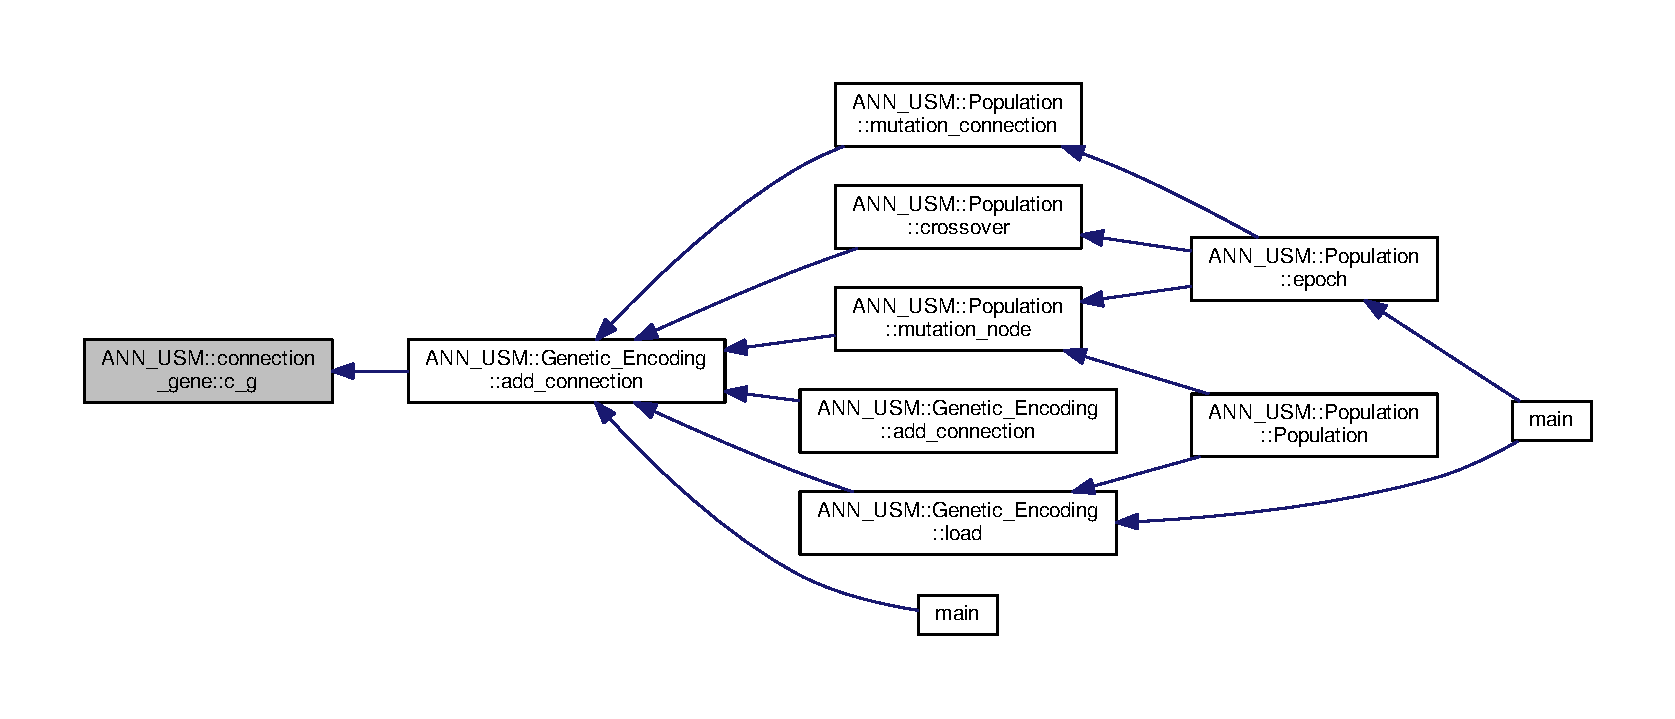
\includegraphics[width=350pt]{class_a_n_n___u_s_m_1_1connection__gene_a48a26d3795acd28e5448a2f542289729_icgraph}
\end{center}
\end{figure}


\hypertarget{class_a_n_n___u_s_m_1_1connection__gene_aa1d7dbb4900169b5b20428188e4f38ff}{\index{A\-N\-N\-\_\-\-U\-S\-M\-::connection\-\_\-gene@{A\-N\-N\-\_\-\-U\-S\-M\-::connection\-\_\-gene}!kill@{kill}}
\index{kill@{kill}!ANN_USM::connection_gene@{A\-N\-N\-\_\-\-U\-S\-M\-::connection\-\_\-gene}}
\subsubsection[{kill}]{\setlength{\rightskip}{0pt plus 5cm}void connection\-\_\-gene\-::kill (
\begin{DoxyParamCaption}
{}
\end{DoxyParamCaption}
)}}\label{class_a_n_n___u_s_m_1_1connection__gene_aa1d7dbb4900169b5b20428188e4f38ff}


Definition at line 25 of file genetic\-\_\-encoding.\-cpp.



Here is the caller graph for this function\-:\nopagebreak
\begin{figure}[H]
\begin{center}
\leavevmode
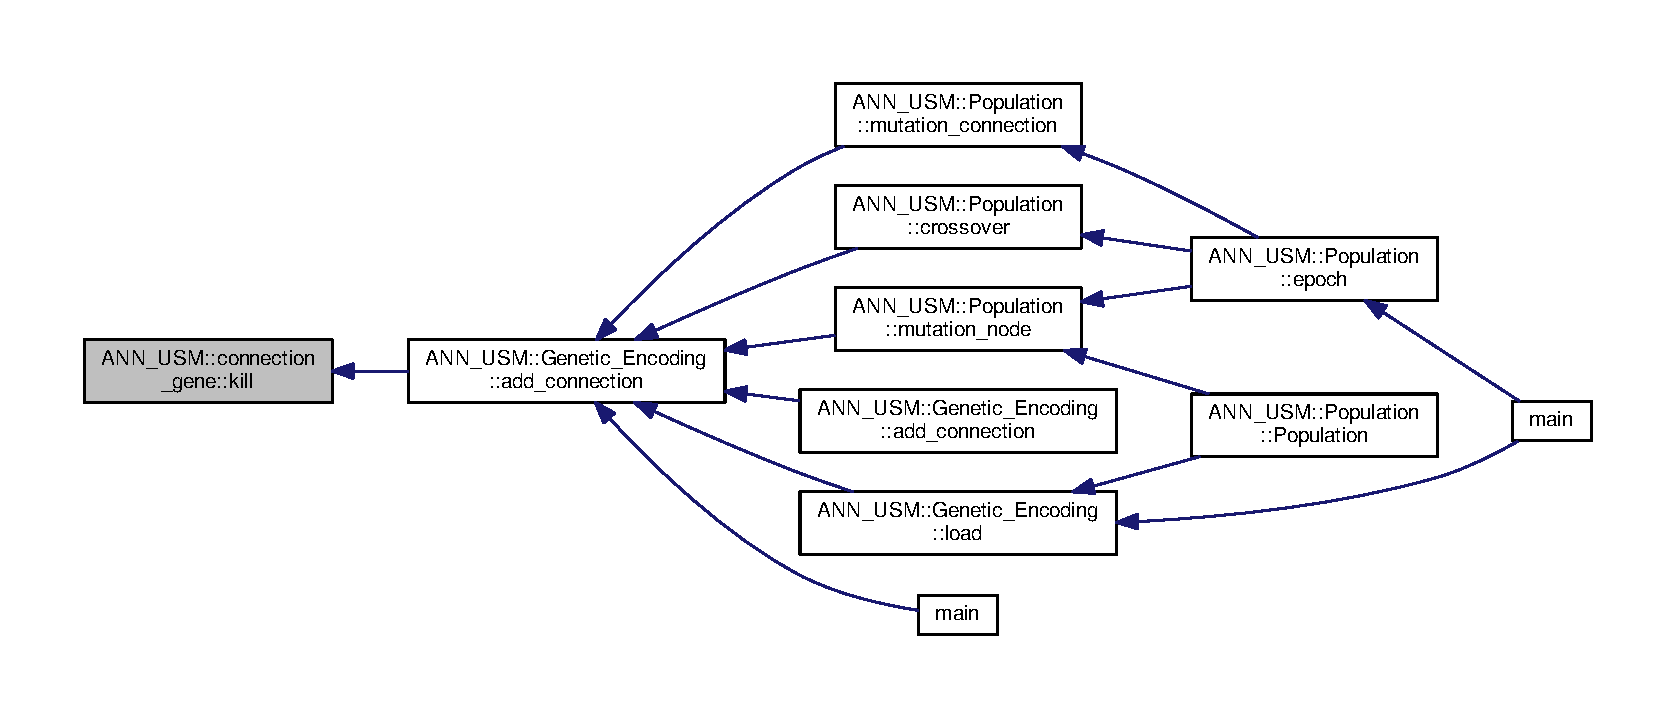
\includegraphics[width=350pt]{class_a_n_n___u_s_m_1_1connection__gene_aa1d7dbb4900169b5b20428188e4f38ff_icgraph}
\end{center}
\end{figure}




\subsection{Member Data Documentation}
\hypertarget{class_a_n_n___u_s_m_1_1connection__gene_ae875a9ba44fa1c534a6e799d4ca64399}{\index{A\-N\-N\-\_\-\-U\-S\-M\-::connection\-\_\-gene@{A\-N\-N\-\_\-\-U\-S\-M\-::connection\-\_\-gene}!enable@{enable}}
\index{enable@{enable}!ANN_USM::connection_gene@{A\-N\-N\-\_\-\-U\-S\-M\-::connection\-\_\-gene}}
\subsubsection[{enable}]{\setlength{\rightskip}{0pt plus 5cm}bool A\-N\-N\-\_\-\-U\-S\-M\-::connection\-\_\-gene\-::enable}}\label{class_a_n_n___u_s_m_1_1connection__gene_ae875a9ba44fa1c534a6e799d4ca64399}


Definition at line 41 of file genetic\-\_\-encoding.\-hpp.

\hypertarget{class_a_n_n___u_s_m_1_1connection__gene_afe8be67cb9aaffbe9015729fbcfe84f9}{\index{A\-N\-N\-\_\-\-U\-S\-M\-::connection\-\_\-gene@{A\-N\-N\-\_\-\-U\-S\-M\-::connection\-\_\-gene}!exist@{exist}}
\index{exist@{exist}!ANN_USM::connection_gene@{A\-N\-N\-\_\-\-U\-S\-M\-::connection\-\_\-gene}}
\subsubsection[{exist}]{\setlength{\rightskip}{0pt plus 5cm}bool A\-N\-N\-\_\-\-U\-S\-M\-::connection\-\_\-gene\-::exist}}\label{class_a_n_n___u_s_m_1_1connection__gene_afe8be67cb9aaffbe9015729fbcfe84f9}


Definition at line 43 of file genetic\-\_\-encoding.\-hpp.

\hypertarget{class_a_n_n___u_s_m_1_1connection__gene_a5100dadf9e141335a47230003303f2d2}{\index{A\-N\-N\-\_\-\-U\-S\-M\-::connection\-\_\-gene@{A\-N\-N\-\_\-\-U\-S\-M\-::connection\-\_\-gene}!in@{in}}
\index{in@{in}!ANN_USM::connection_gene@{A\-N\-N\-\_\-\-U\-S\-M\-::connection\-\_\-gene}}
\subsubsection[{in}]{\setlength{\rightskip}{0pt plus 5cm}int A\-N\-N\-\_\-\-U\-S\-M\-::connection\-\_\-gene\-::in}}\label{class_a_n_n___u_s_m_1_1connection__gene_a5100dadf9e141335a47230003303f2d2}


Definition at line 39 of file genetic\-\_\-encoding.\-hpp.

\hypertarget{class_a_n_n___u_s_m_1_1connection__gene_acd19e4cadbac4ef5aa4ae0b7aa3ae5c2}{\index{A\-N\-N\-\_\-\-U\-S\-M\-::connection\-\_\-gene@{A\-N\-N\-\_\-\-U\-S\-M\-::connection\-\_\-gene}!innovation@{innovation}}
\index{innovation@{innovation}!ANN_USM::connection_gene@{A\-N\-N\-\_\-\-U\-S\-M\-::connection\-\_\-gene}}
\subsubsection[{innovation}]{\setlength{\rightskip}{0pt plus 5cm}int A\-N\-N\-\_\-\-U\-S\-M\-::connection\-\_\-gene\-::innovation}}\label{class_a_n_n___u_s_m_1_1connection__gene_acd19e4cadbac4ef5aa4ae0b7aa3ae5c2}


Definition at line 38 of file genetic\-\_\-encoding.\-hpp.

\hypertarget{class_a_n_n___u_s_m_1_1connection__gene_abc6a5dafbfa3133efc876c8f0f762dd6}{\index{A\-N\-N\-\_\-\-U\-S\-M\-::connection\-\_\-gene@{A\-N\-N\-\_\-\-U\-S\-M\-::connection\-\_\-gene}!out@{out}}
\index{out@{out}!ANN_USM::connection_gene@{A\-N\-N\-\_\-\-U\-S\-M\-::connection\-\_\-gene}}
\subsubsection[{out}]{\setlength{\rightskip}{0pt plus 5cm}int A\-N\-N\-\_\-\-U\-S\-M\-::connection\-\_\-gene\-::out}}\label{class_a_n_n___u_s_m_1_1connection__gene_abc6a5dafbfa3133efc876c8f0f762dd6}


Definition at line 40 of file genetic\-\_\-encoding.\-hpp.

\hypertarget{class_a_n_n___u_s_m_1_1connection__gene_a12dddd6cd3c0c5b9749015cc1c81e480}{\index{A\-N\-N\-\_\-\-U\-S\-M\-::connection\-\_\-gene@{A\-N\-N\-\_\-\-U\-S\-M\-::connection\-\_\-gene}!weight@{weight}}
\index{weight@{weight}!ANN_USM::connection_gene@{A\-N\-N\-\_\-\-U\-S\-M\-::connection\-\_\-gene}}
\subsubsection[{weight}]{\setlength{\rightskip}{0pt plus 5cm}double A\-N\-N\-\_\-\-U\-S\-M\-::connection\-\_\-gene\-::weight}}\label{class_a_n_n___u_s_m_1_1connection__gene_a12dddd6cd3c0c5b9749015cc1c81e480}


Definition at line 42 of file genetic\-\_\-encoding.\-hpp.



The documentation for this class was generated from the following files\-:\begin{DoxyCompactItemize}
\item 
headers/\hyperlink{genetic__encoding_8hpp}{genetic\-\_\-encoding.\-hpp}\item 
src/\hyperlink{genetic__encoding_8cpp}{genetic\-\_\-encoding.\-cpp}\end{DoxyCompactItemize}

\hypertarget{class_function}{\section{Function Class Reference}
\label{class_function}\index{Function@{Function}}
}


{\ttfamily \#include $<$function.\-hpp$>$}

\subsection*{Public Member Functions}
\begin{DoxyCompactItemize}
\item 
\hyperlink{class_function_ae206568fd4fd4c885e3ccff76345c4e6}{Function} ()
\item 
\hyperlink{class_function_a2e61bc024c6b551a91d0cee230e394a7}{Function} (string)
\item 
double \hyperlink{class_function_adeb29c59e42bf4431912f2a6484b1ad9}{eval} (double)
\item 
string \hyperlink{class_function_a2738abb4d98326b3789ad2b0ad44dfd8}{get\-\_\-name} (int function)
\item 
string \hyperlink{class_function_ad180cc43d0d7bb5e4b2cf5242c734d3c}{get\-\_\-name} ()
\end{DoxyCompactItemize}


\subsection{Detailed Description}


Definition at line 11 of file function.\-hpp.



\subsection{Constructor \& Destructor Documentation}
\hypertarget{class_function_ae206568fd4fd4c885e3ccff76345c4e6}{\index{Function@{Function}!Function@{Function}}
\index{Function@{Function}!Function@{Function}}
\subsubsection[{Function}]{\setlength{\rightskip}{0pt plus 5cm}Function\-::\-Function (
\begin{DoxyParamCaption}
{}
\end{DoxyParamCaption}
)}}\label{class_function_ae206568fd4fd4c885e3ccff76345c4e6}


Definition at line 5 of file function.\-cpp.

\hypertarget{class_function_a2e61bc024c6b551a91d0cee230e394a7}{\index{Function@{Function}!Function@{Function}}
\index{Function@{Function}!Function@{Function}}
\subsubsection[{Function}]{\setlength{\rightskip}{0pt plus 5cm}Function\-::\-Function (
\begin{DoxyParamCaption}
\item[{string}]{function\-\_\-name}
\end{DoxyParamCaption}
)}}\label{class_function_a2e61bc024c6b551a91d0cee230e394a7}


Definition at line 7 of file function.\-cpp.



\subsection{Member Function Documentation}
\hypertarget{class_function_adeb29c59e42bf4431912f2a6484b1ad9}{\index{Function@{Function}!eval@{eval}}
\index{eval@{eval}!Function@{Function}}
\subsubsection[{eval}]{\setlength{\rightskip}{0pt plus 5cm}double Function\-::eval (
\begin{DoxyParamCaption}
\item[{double}]{input}
\end{DoxyParamCaption}
)}}\label{class_function_adeb29c59e42bf4431912f2a6484b1ad9}


Definition at line 36 of file function.\-cpp.

\hypertarget{class_function_a2738abb4d98326b3789ad2b0ad44dfd8}{\index{Function@{Function}!get\-\_\-name@{get\-\_\-name}}
\index{get\-\_\-name@{get\-\_\-name}!Function@{Function}}
\subsubsection[{get\-\_\-name}]{\setlength{\rightskip}{0pt plus 5cm}string Function\-::get\-\_\-name (
\begin{DoxyParamCaption}
\item[{int}]{function}
\end{DoxyParamCaption}
)}}\label{class_function_a2738abb4d98326b3789ad2b0ad44dfd8}


Definition at line 41 of file function.\-cpp.



Here is the caller graph for this function\-:\nopagebreak
\begin{figure}[H]
\begin{center}
\leavevmode
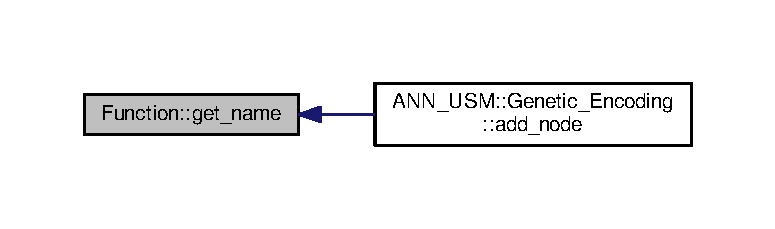
\includegraphics[width=350pt]{class_function_a2738abb4d98326b3789ad2b0ad44dfd8_icgraph}
\end{center}
\end{figure}


\hypertarget{class_function_ad180cc43d0d7bb5e4b2cf5242c734d3c}{\index{Function@{Function}!get\-\_\-name@{get\-\_\-name}}
\index{get\-\_\-name@{get\-\_\-name}!Function@{Function}}
\subsubsection[{get\-\_\-name}]{\setlength{\rightskip}{0pt plus 5cm}string Function\-::get\-\_\-name (
\begin{DoxyParamCaption}
{}
\end{DoxyParamCaption}
)}}\label{class_function_ad180cc43d0d7bb5e4b2cf5242c734d3c}


Definition at line 59 of file function.\-cpp.



The documentation for this class was generated from the following files\-:\begin{DoxyCompactItemize}
\item 
headers/\hyperlink{function_8hpp}{function.\-hpp}\item 
src/\hyperlink{function_8cpp}{function.\-cpp}\end{DoxyCompactItemize}

\hypertarget{class_a_n_n___u_s_m_1_1_genetic___encoding}{\section{A\-N\-N\-\_\-\-U\-S\-M\-:\-:Genetic\-\_\-\-Encoding Class Reference}
\label{class_a_n_n___u_s_m_1_1_genetic___encoding}\index{A\-N\-N\-\_\-\-U\-S\-M\-::\-Genetic\-\_\-\-Encoding@{A\-N\-N\-\_\-\-U\-S\-M\-::\-Genetic\-\_\-\-Encoding}}
}


{\ttfamily \#include $<$genetic\-\_\-encoding.\-hpp$>$}

\subsection*{Public Member Functions}
\begin{DoxyCompactItemize}
\item 
void \hyperlink{class_a_n_n___u_s_m_1_1_genetic___encoding_a1451a90f4672e672dc559f6f5f78a9f0}{add\-\_\-node} (int node, int row, \hyperlink{namespace_a_n_n___u_s_m_aa7f97f486244dd898592ba14dd7aa778}{gene\-\_\-type} type, string function)
\item 
void \hyperlink{class_a_n_n___u_s_m_1_1_genetic___encoding_aee703abc7c6549f4b1d8f6c968ade23d}{add\-\_\-node} (\hyperlink{class_a_n_n___u_s_m_1_1node__gene}{node\-\_\-gene} node)
\item 
void \hyperlink{class_a_n_n___u_s_m_1_1_genetic___encoding_a4e46296d0531840686d8a0e6927c3eae}{add\-\_\-connection} (int innovation, int in, int out, double weight, bool enable)
\item 
void \hyperlink{class_a_n_n___u_s_m_1_1_genetic___encoding_a58aae26273d906a268974b3e32e830eb}{add\-\_\-connection} (\hyperlink{class_a_n_n___u_s_m_1_1connection__gene}{connection\-\_\-gene} conn)
\item 
void \hyperlink{class_a_n_n___u_s_m_1_1_genetic___encoding_a10660e165ed513e7e19cee375ea7de88}{change\-\_\-weight} (int innovation, double weight)
\item 
void \hyperlink{class_a_n_n___u_s_m_1_1_genetic___encoding_a4b008853b6cdb594f932d3d2fd8679dd}{save} (char path\mbox{[}$\,$\mbox{]})
\item 
void \hyperlink{class_a_n_n___u_s_m_1_1_genetic___encoding_aa02f2917484681f2ea7de654c8de1ed4}{load} (char path\mbox{[}$\,$\mbox{]})
\item 
void \hyperlink{class_a_n_n___u_s_m_1_1_genetic___encoding_ab861af85462942c5238567496fe6def0}{spread\-\_\-final\-\_\-result} (int node, double value)
\item 
string \hyperlink{class_a_n_n___u_s_m_1_1_genetic___encoding_a6e047636ec1196cba5d6240ff2dd589f}{J\-S\-O\-N} ()
\item 
vector$<$ double $>$ \hyperlink{class_a_n_n___u_s_m_1_1_genetic___encoding_a31b9ed6ea6134b1ddc27446575e69d1a}{eval} (vector$<$ double $>$ inputs)
\end{DoxyCompactItemize}
\subsection*{Public Attributes}
\begin{DoxyCompactItemize}
\item 
vector$<$ \hyperlink{class_a_n_n___u_s_m_1_1connection__gene}{connection\-\_\-gene} $>$ \hyperlink{class_a_n_n___u_s_m_1_1_genetic___encoding_a4396b8b09edcd7be7714cebf1df17742}{Lconnection\-\_\-genes}
\item 
vector$<$ \hyperlink{class_a_n_n___u_s_m_1_1node__gene}{node\-\_\-gene} $>$ \hyperlink{class_a_n_n___u_s_m_1_1_genetic___encoding_a2afdafa9f3c396f1ffeee7c0c4a2269e}{Lnode\-\_\-genes}
\item 
vector$<$ int $>$ \hyperlink{class_a_n_n___u_s_m_1_1_genetic___encoding_a5afe8e6c6ab62610aa5b239f19b1ee3c}{input\-\_\-nodes}
\item 
vector$<$ int $>$ \hyperlink{class_a_n_n___u_s_m_1_1_genetic___encoding_a66ce2a57061f434146f6a797105ea96f}{output\-\_\-nodes}
\item 
vector$<$ int $>$ \hyperlink{class_a_n_n___u_s_m_1_1_genetic___encoding_a410de772c609b972f6ec913e81b7d797}{row\-\_\-orderer\-\_\-list}
\item 
int \hyperlink{class_a_n_n___u_s_m_1_1_genetic___encoding_ab7d9c478bd171ad0e522298c42fe6ba9}{niche}
\end{DoxyCompactItemize}


\subsection{Detailed Description}


Definition at line 88 of file genetic\-\_\-encoding.\-hpp.



\subsection{Member Function Documentation}
\hypertarget{class_a_n_n___u_s_m_1_1_genetic___encoding_a4e46296d0531840686d8a0e6927c3eae}{\index{A\-N\-N\-\_\-\-U\-S\-M\-::\-Genetic\-\_\-\-Encoding@{A\-N\-N\-\_\-\-U\-S\-M\-::\-Genetic\-\_\-\-Encoding}!add\-\_\-connection@{add\-\_\-connection}}
\index{add\-\_\-connection@{add\-\_\-connection}!ANN_USM::Genetic_Encoding@{A\-N\-N\-\_\-\-U\-S\-M\-::\-Genetic\-\_\-\-Encoding}}
\subsubsection[{add\-\_\-connection}]{\setlength{\rightskip}{0pt plus 5cm}void Genetic\-\_\-\-Encoding\-::add\-\_\-connection (
\begin{DoxyParamCaption}
\item[{int}]{innovation, }
\item[{int}]{in, }
\item[{int}]{out, }
\item[{double}]{weight, }
\item[{bool}]{enable}
\end{DoxyParamCaption}
)}}\label{class_a_n_n___u_s_m_1_1_genetic___encoding_a4e46296d0531840686d8a0e6927c3eae}


Definition at line 100 of file genetic\-\_\-encoding.\-cpp.



Here is the call graph for this function\-:\nopagebreak
\begin{figure}[H]
\begin{center}
\leavevmode
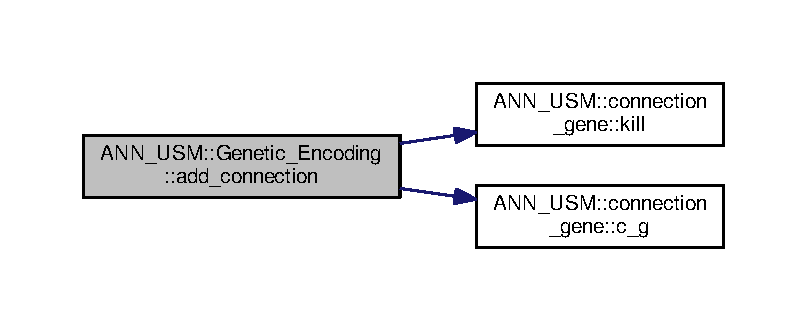
\includegraphics[width=350pt]{class_a_n_n___u_s_m_1_1_genetic___encoding_a4e46296d0531840686d8a0e6927c3eae_cgraph}
\end{center}
\end{figure}




Here is the caller graph for this function\-:\nopagebreak
\begin{figure}[H]
\begin{center}
\leavevmode
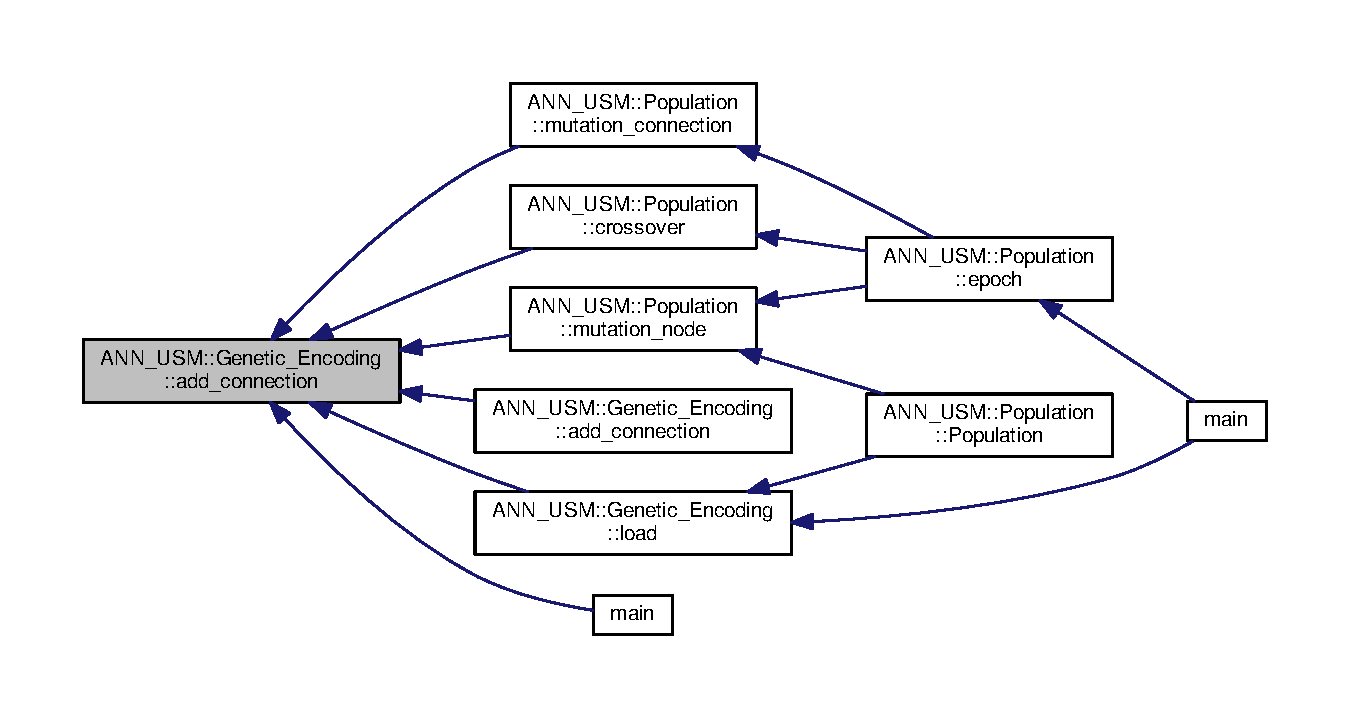
\includegraphics[width=350pt]{class_a_n_n___u_s_m_1_1_genetic___encoding_a4e46296d0531840686d8a0e6927c3eae_icgraph}
\end{center}
\end{figure}


\hypertarget{class_a_n_n___u_s_m_1_1_genetic___encoding_a58aae26273d906a268974b3e32e830eb}{\index{A\-N\-N\-\_\-\-U\-S\-M\-::\-Genetic\-\_\-\-Encoding@{A\-N\-N\-\_\-\-U\-S\-M\-::\-Genetic\-\_\-\-Encoding}!add\-\_\-connection@{add\-\_\-connection}}
\index{add\-\_\-connection@{add\-\_\-connection}!ANN_USM::Genetic_Encoding@{A\-N\-N\-\_\-\-U\-S\-M\-::\-Genetic\-\_\-\-Encoding}}
\subsubsection[{add\-\_\-connection}]{\setlength{\rightskip}{0pt plus 5cm}void Genetic\-\_\-\-Encoding\-::add\-\_\-connection (
\begin{DoxyParamCaption}
\item[{{\bf connection\-\_\-gene}}]{conn}
\end{DoxyParamCaption}
)}}\label{class_a_n_n___u_s_m_1_1_genetic___encoding_a58aae26273d906a268974b3e32e830eb}


Definition at line 95 of file genetic\-\_\-encoding.\-cpp.



Here is the call graph for this function\-:\nopagebreak
\begin{figure}[H]
\begin{center}
\leavevmode
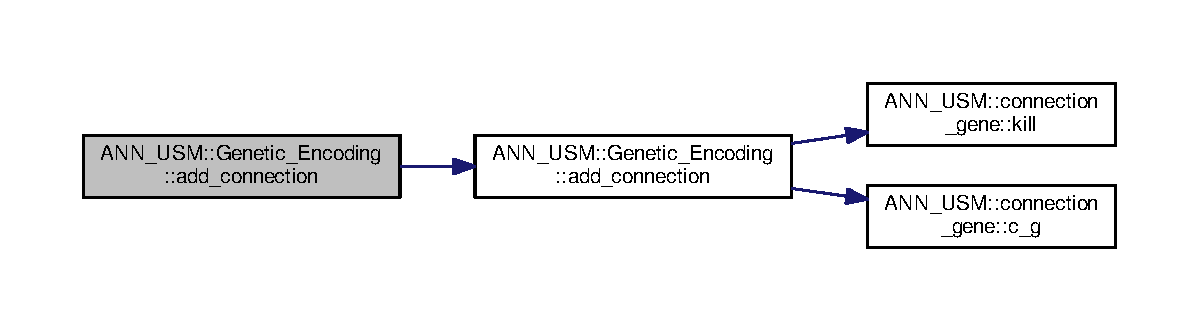
\includegraphics[width=350pt]{class_a_n_n___u_s_m_1_1_genetic___encoding_a58aae26273d906a268974b3e32e830eb_cgraph}
\end{center}
\end{figure}


\hypertarget{class_a_n_n___u_s_m_1_1_genetic___encoding_a1451a90f4672e672dc559f6f5f78a9f0}{\index{A\-N\-N\-\_\-\-U\-S\-M\-::\-Genetic\-\_\-\-Encoding@{A\-N\-N\-\_\-\-U\-S\-M\-::\-Genetic\-\_\-\-Encoding}!add\-\_\-node@{add\-\_\-node}}
\index{add\-\_\-node@{add\-\_\-node}!ANN_USM::Genetic_Encoding@{A\-N\-N\-\_\-\-U\-S\-M\-::\-Genetic\-\_\-\-Encoding}}
\subsubsection[{add\-\_\-node}]{\setlength{\rightskip}{0pt plus 5cm}void Genetic\-\_\-\-Encoding\-::add\-\_\-node (
\begin{DoxyParamCaption}
\item[{int}]{node, }
\item[{int}]{row, }
\item[{{\bf gene\-\_\-type}}]{type, }
\item[{string}]{function}
\end{DoxyParamCaption}
)}}\label{class_a_n_n___u_s_m_1_1_genetic___encoding_a1451a90f4672e672dc559f6f5f78a9f0}


Definition at line 145 of file genetic\-\_\-encoding.\-cpp.



Here is the call graph for this function\-:\nopagebreak
\begin{figure}[H]
\begin{center}
\leavevmode
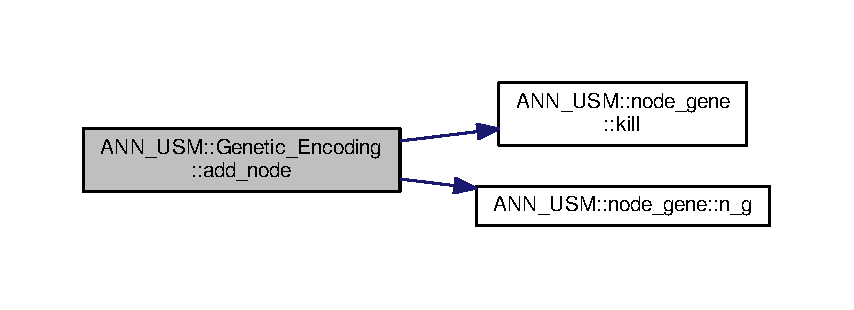
\includegraphics[width=350pt]{class_a_n_n___u_s_m_1_1_genetic___encoding_a1451a90f4672e672dc559f6f5f78a9f0_cgraph}
\end{center}
\end{figure}




Here is the caller graph for this function\-:\nopagebreak
\begin{figure}[H]
\begin{center}
\leavevmode
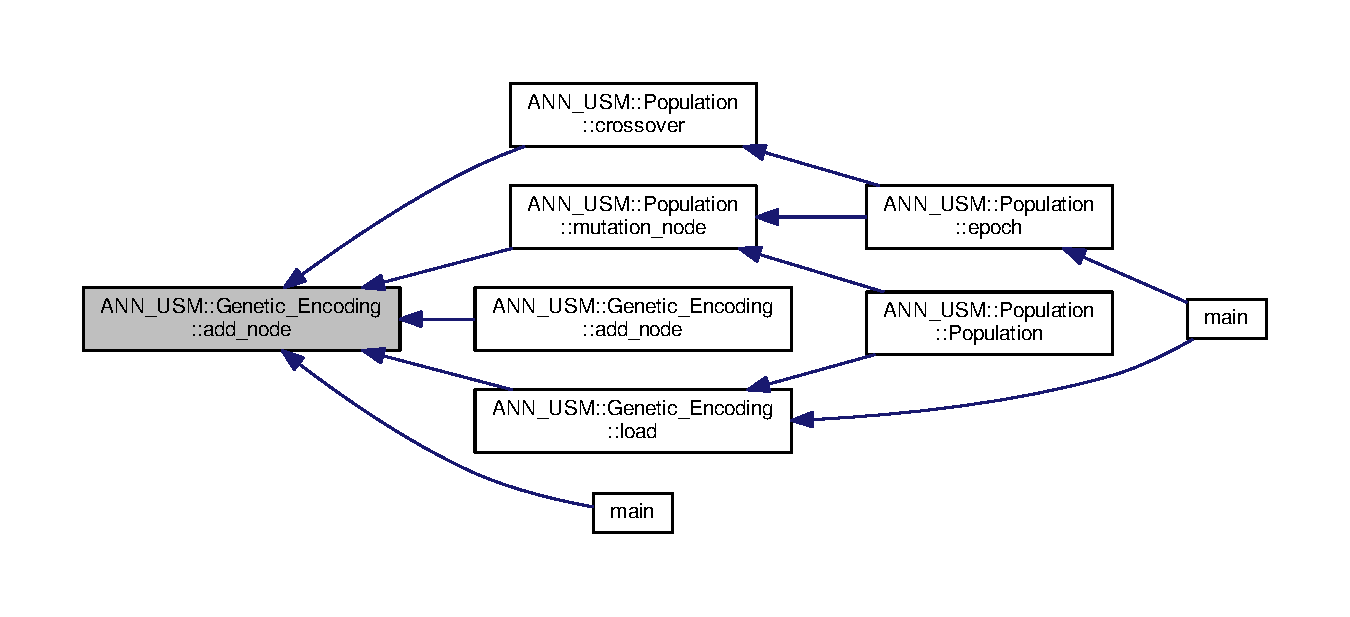
\includegraphics[width=350pt]{class_a_n_n___u_s_m_1_1_genetic___encoding_a1451a90f4672e672dc559f6f5f78a9f0_icgraph}
\end{center}
\end{figure}


\hypertarget{class_a_n_n___u_s_m_1_1_genetic___encoding_aee703abc7c6549f4b1d8f6c968ade23d}{\index{A\-N\-N\-\_\-\-U\-S\-M\-::\-Genetic\-\_\-\-Encoding@{A\-N\-N\-\_\-\-U\-S\-M\-::\-Genetic\-\_\-\-Encoding}!add\-\_\-node@{add\-\_\-node}}
\index{add\-\_\-node@{add\-\_\-node}!ANN_USM::Genetic_Encoding@{A\-N\-N\-\_\-\-U\-S\-M\-::\-Genetic\-\_\-\-Encoding}}
\subsubsection[{add\-\_\-node}]{\setlength{\rightskip}{0pt plus 5cm}void Genetic\-\_\-\-Encoding\-::add\-\_\-node (
\begin{DoxyParamCaption}
\item[{{\bf node\-\_\-gene}}]{node}
\end{DoxyParamCaption}
)}}\label{class_a_n_n___u_s_m_1_1_genetic___encoding_aee703abc7c6549f4b1d8f6c968ade23d}


Definition at line 140 of file genetic\-\_\-encoding.\-cpp.



Here is the call graph for this function\-:\nopagebreak
\begin{figure}[H]
\begin{center}
\leavevmode
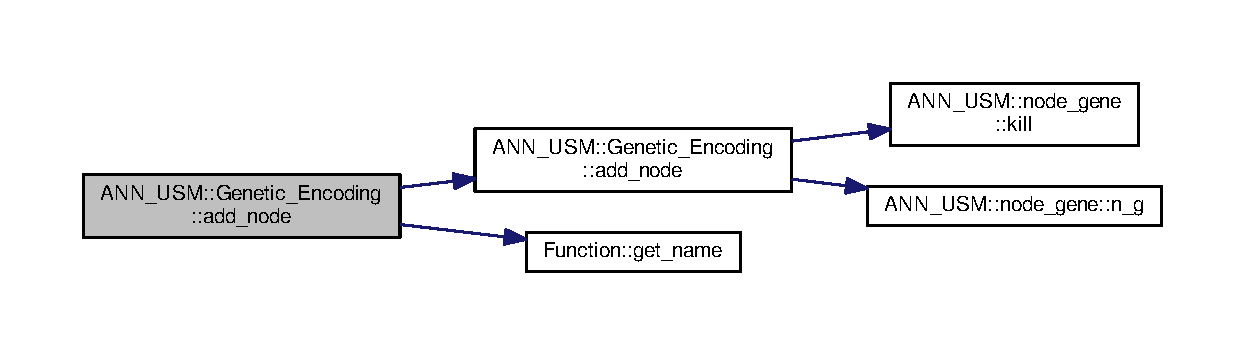
\includegraphics[width=350pt]{class_a_n_n___u_s_m_1_1_genetic___encoding_aee703abc7c6549f4b1d8f6c968ade23d_cgraph}
\end{center}
\end{figure}


\hypertarget{class_a_n_n___u_s_m_1_1_genetic___encoding_a10660e165ed513e7e19cee375ea7de88}{\index{A\-N\-N\-\_\-\-U\-S\-M\-::\-Genetic\-\_\-\-Encoding@{A\-N\-N\-\_\-\-U\-S\-M\-::\-Genetic\-\_\-\-Encoding}!change\-\_\-weight@{change\-\_\-weight}}
\index{change\-\_\-weight@{change\-\_\-weight}!ANN_USM::Genetic_Encoding@{A\-N\-N\-\_\-\-U\-S\-M\-::\-Genetic\-\_\-\-Encoding}}
\subsubsection[{change\-\_\-weight}]{\setlength{\rightskip}{0pt plus 5cm}void A\-N\-N\-\_\-\-U\-S\-M\-::\-Genetic\-\_\-\-Encoding\-::change\-\_\-weight (
\begin{DoxyParamCaption}
\item[{int}]{innovation, }
\item[{double}]{weight}
\end{DoxyParamCaption}
)}}\label{class_a_n_n___u_s_m_1_1_genetic___encoding_a10660e165ed513e7e19cee375ea7de88}
\hypertarget{class_a_n_n___u_s_m_1_1_genetic___encoding_a31b9ed6ea6134b1ddc27446575e69d1a}{\index{A\-N\-N\-\_\-\-U\-S\-M\-::\-Genetic\-\_\-\-Encoding@{A\-N\-N\-\_\-\-U\-S\-M\-::\-Genetic\-\_\-\-Encoding}!eval@{eval}}
\index{eval@{eval}!ANN_USM::Genetic_Encoding@{A\-N\-N\-\_\-\-U\-S\-M\-::\-Genetic\-\_\-\-Encoding}}
\subsubsection[{eval}]{\setlength{\rightskip}{0pt plus 5cm}vector$<$ double $>$ Genetic\-\_\-\-Encoding\-::eval (
\begin{DoxyParamCaption}
\item[{vector$<$ double $>$}]{inputs}
\end{DoxyParamCaption}
)}}\label{class_a_n_n___u_s_m_1_1_genetic___encoding_a31b9ed6ea6134b1ddc27446575e69d1a}


Definition at line 186 of file genetic\-\_\-encoding.\-cpp.



Here is the call graph for this function\-:\nopagebreak
\begin{figure}[H]
\begin{center}
\leavevmode
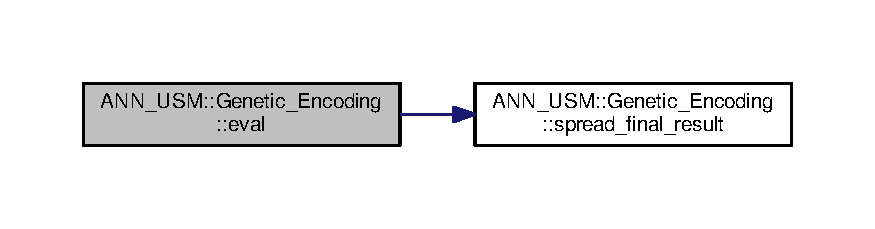
\includegraphics[width=350pt]{class_a_n_n___u_s_m_1_1_genetic___encoding_a31b9ed6ea6134b1ddc27446575e69d1a_cgraph}
\end{center}
\end{figure}




Here is the caller graph for this function\-:\nopagebreak
\begin{figure}[H]
\begin{center}
\leavevmode
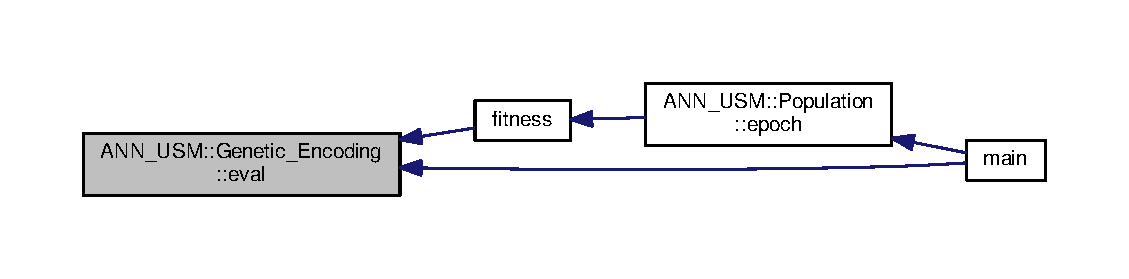
\includegraphics[width=350pt]{class_a_n_n___u_s_m_1_1_genetic___encoding_a31b9ed6ea6134b1ddc27446575e69d1a_icgraph}
\end{center}
\end{figure}


\hypertarget{class_a_n_n___u_s_m_1_1_genetic___encoding_a6e047636ec1196cba5d6240ff2dd589f}{\index{A\-N\-N\-\_\-\-U\-S\-M\-::\-Genetic\-\_\-\-Encoding@{A\-N\-N\-\_\-\-U\-S\-M\-::\-Genetic\-\_\-\-Encoding}!J\-S\-O\-N@{J\-S\-O\-N}}
\index{J\-S\-O\-N@{J\-S\-O\-N}!ANN_USM::Genetic_Encoding@{A\-N\-N\-\_\-\-U\-S\-M\-::\-Genetic\-\_\-\-Encoding}}
\subsubsection[{J\-S\-O\-N}]{\setlength{\rightskip}{0pt plus 5cm}string Genetic\-\_\-\-Encoding\-::\-J\-S\-O\-N (
\begin{DoxyParamCaption}
{}
\end{DoxyParamCaption}
)}}\label{class_a_n_n___u_s_m_1_1_genetic___encoding_a6e047636ec1196cba5d6240ff2dd589f}


Definition at line 246 of file genetic\-\_\-encoding.\-cpp.



Here is the caller graph for this function\-:\nopagebreak
\begin{figure}[H]
\begin{center}
\leavevmode
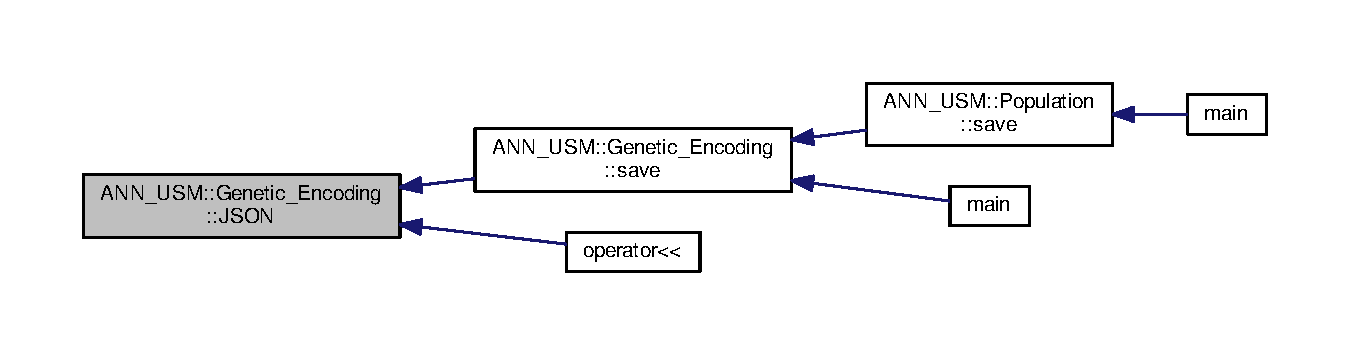
\includegraphics[width=350pt]{class_a_n_n___u_s_m_1_1_genetic___encoding_a6e047636ec1196cba5d6240ff2dd589f_icgraph}
\end{center}
\end{figure}


\hypertarget{class_a_n_n___u_s_m_1_1_genetic___encoding_aa02f2917484681f2ea7de654c8de1ed4}{\index{A\-N\-N\-\_\-\-U\-S\-M\-::\-Genetic\-\_\-\-Encoding@{A\-N\-N\-\_\-\-U\-S\-M\-::\-Genetic\-\_\-\-Encoding}!load@{load}}
\index{load@{load}!ANN_USM::Genetic_Encoding@{A\-N\-N\-\_\-\-U\-S\-M\-::\-Genetic\-\_\-\-Encoding}}
\subsubsection[{load}]{\setlength{\rightskip}{0pt plus 5cm}void Genetic\-\_\-\-Encoding\-::load (
\begin{DoxyParamCaption}
\item[{char}]{path\mbox{[}$\,$\mbox{]}}
\end{DoxyParamCaption}
)}}\label{class_a_n_n___u_s_m_1_1_genetic___encoding_aa02f2917484681f2ea7de654c8de1ed4}


Definition at line 298 of file genetic\-\_\-encoding.\-cpp.



Here is the call graph for this function\-:\nopagebreak
\begin{figure}[H]
\begin{center}
\leavevmode
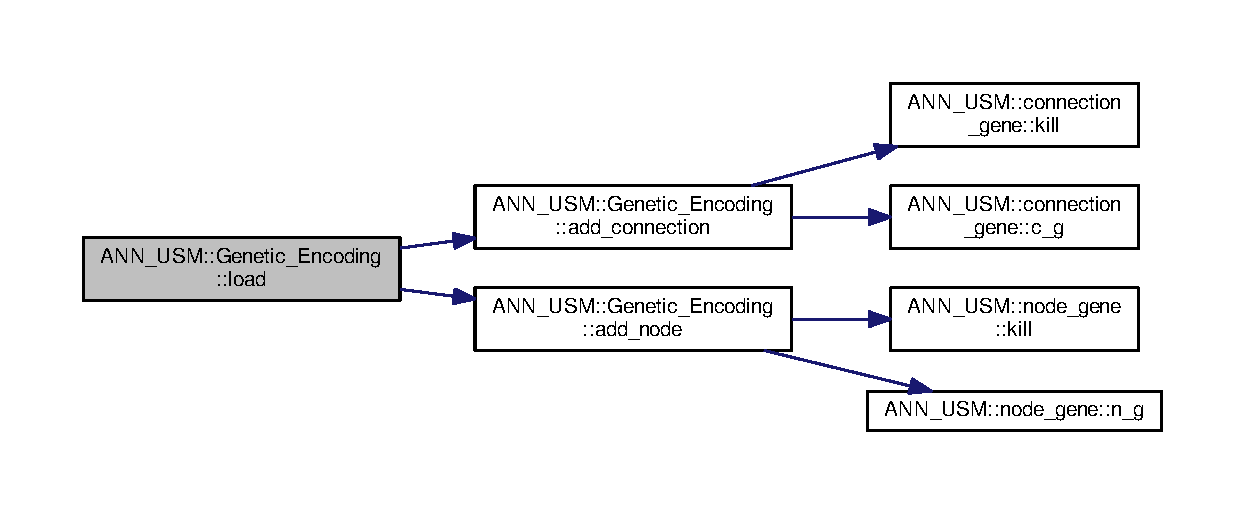
\includegraphics[width=350pt]{class_a_n_n___u_s_m_1_1_genetic___encoding_aa02f2917484681f2ea7de654c8de1ed4_cgraph}
\end{center}
\end{figure}




Here is the caller graph for this function\-:\nopagebreak
\begin{figure}[H]
\begin{center}
\leavevmode
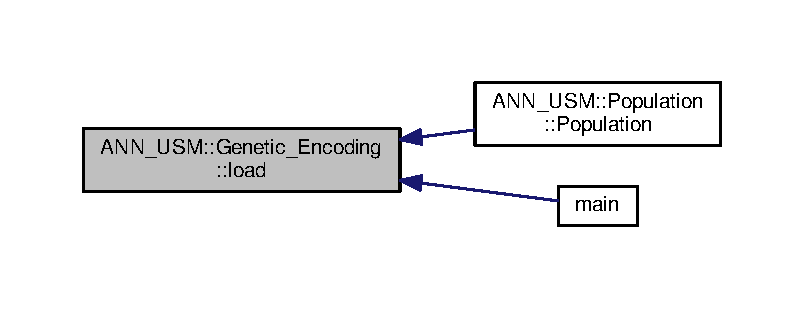
\includegraphics[width=350pt]{class_a_n_n___u_s_m_1_1_genetic___encoding_aa02f2917484681f2ea7de654c8de1ed4_icgraph}
\end{center}
\end{figure}


\hypertarget{class_a_n_n___u_s_m_1_1_genetic___encoding_a4b008853b6cdb594f932d3d2fd8679dd}{\index{A\-N\-N\-\_\-\-U\-S\-M\-::\-Genetic\-\_\-\-Encoding@{A\-N\-N\-\_\-\-U\-S\-M\-::\-Genetic\-\_\-\-Encoding}!save@{save}}
\index{save@{save}!ANN_USM::Genetic_Encoding@{A\-N\-N\-\_\-\-U\-S\-M\-::\-Genetic\-\_\-\-Encoding}}
\subsubsection[{save}]{\setlength{\rightskip}{0pt plus 5cm}void Genetic\-\_\-\-Encoding\-::save (
\begin{DoxyParamCaption}
\item[{char}]{path\mbox{[}$\,$\mbox{]}}
\end{DoxyParamCaption}
)}}\label{class_a_n_n___u_s_m_1_1_genetic___encoding_a4b008853b6cdb594f932d3d2fd8679dd}


Definition at line 290 of file genetic\-\_\-encoding.\-cpp.



Here is the call graph for this function\-:\nopagebreak
\begin{figure}[H]
\begin{center}
\leavevmode
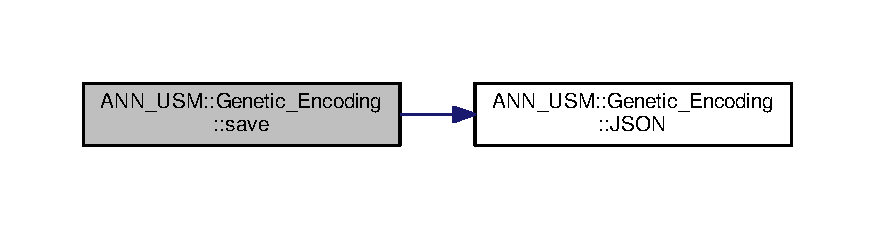
\includegraphics[width=350pt]{class_a_n_n___u_s_m_1_1_genetic___encoding_a4b008853b6cdb594f932d3d2fd8679dd_cgraph}
\end{center}
\end{figure}




Here is the caller graph for this function\-:\nopagebreak
\begin{figure}[H]
\begin{center}
\leavevmode
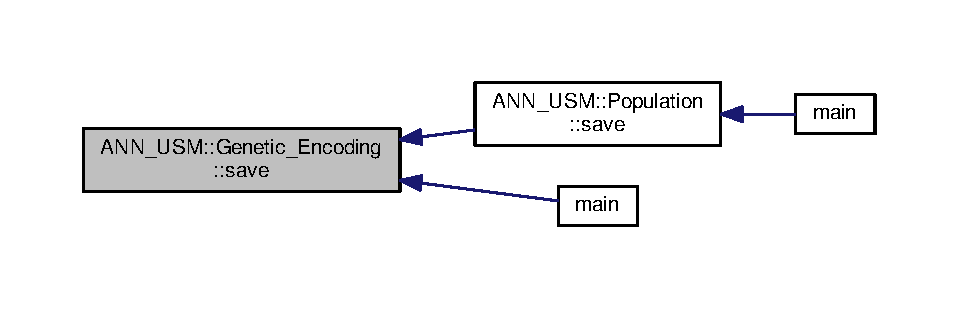
\includegraphics[width=350pt]{class_a_n_n___u_s_m_1_1_genetic___encoding_a4b008853b6cdb594f932d3d2fd8679dd_icgraph}
\end{center}
\end{figure}


\hypertarget{class_a_n_n___u_s_m_1_1_genetic___encoding_ab861af85462942c5238567496fe6def0}{\index{A\-N\-N\-\_\-\-U\-S\-M\-::\-Genetic\-\_\-\-Encoding@{A\-N\-N\-\_\-\-U\-S\-M\-::\-Genetic\-\_\-\-Encoding}!spread\-\_\-final\-\_\-result@{spread\-\_\-final\-\_\-result}}
\index{spread\-\_\-final\-\_\-result@{spread\-\_\-final\-\_\-result}!ANN_USM::Genetic_Encoding@{A\-N\-N\-\_\-\-U\-S\-M\-::\-Genetic\-\_\-\-Encoding}}
\subsubsection[{spread\-\_\-final\-\_\-result}]{\setlength{\rightskip}{0pt plus 5cm}void Genetic\-\_\-\-Encoding\-::spread\-\_\-final\-\_\-result (
\begin{DoxyParamCaption}
\item[{int}]{node, }
\item[{double}]{value}
\end{DoxyParamCaption}
)}}\label{class_a_n_n___u_s_m_1_1_genetic___encoding_ab861af85462942c5238567496fe6def0}


Definition at line 224 of file genetic\-\_\-encoding.\-cpp.



Here is the caller graph for this function\-:\nopagebreak
\begin{figure}[H]
\begin{center}
\leavevmode
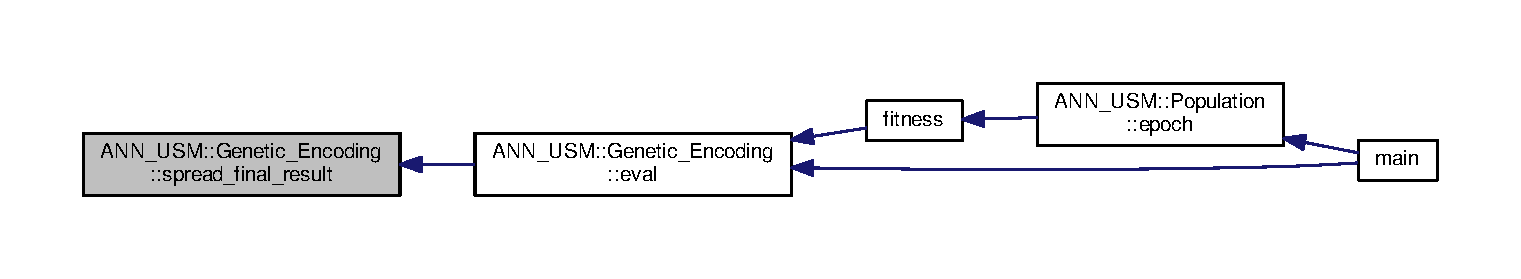
\includegraphics[width=350pt]{class_a_n_n___u_s_m_1_1_genetic___encoding_ab861af85462942c5238567496fe6def0_icgraph}
\end{center}
\end{figure}




\subsection{Member Data Documentation}
\hypertarget{class_a_n_n___u_s_m_1_1_genetic___encoding_a5afe8e6c6ab62610aa5b239f19b1ee3c}{\index{A\-N\-N\-\_\-\-U\-S\-M\-::\-Genetic\-\_\-\-Encoding@{A\-N\-N\-\_\-\-U\-S\-M\-::\-Genetic\-\_\-\-Encoding}!input\-\_\-nodes@{input\-\_\-nodes}}
\index{input\-\_\-nodes@{input\-\_\-nodes}!ANN_USM::Genetic_Encoding@{A\-N\-N\-\_\-\-U\-S\-M\-::\-Genetic\-\_\-\-Encoding}}
\subsubsection[{input\-\_\-nodes}]{\setlength{\rightskip}{0pt plus 5cm}vector$<$int$>$ A\-N\-N\-\_\-\-U\-S\-M\-::\-Genetic\-\_\-\-Encoding\-::input\-\_\-nodes}}\label{class_a_n_n___u_s_m_1_1_genetic___encoding_a5afe8e6c6ab62610aa5b239f19b1ee3c}


Definition at line 111 of file genetic\-\_\-encoding.\-hpp.

\hypertarget{class_a_n_n___u_s_m_1_1_genetic___encoding_a4396b8b09edcd7be7714cebf1df17742}{\index{A\-N\-N\-\_\-\-U\-S\-M\-::\-Genetic\-\_\-\-Encoding@{A\-N\-N\-\_\-\-U\-S\-M\-::\-Genetic\-\_\-\-Encoding}!Lconnection\-\_\-genes@{Lconnection\-\_\-genes}}
\index{Lconnection\-\_\-genes@{Lconnection\-\_\-genes}!ANN_USM::Genetic_Encoding@{A\-N\-N\-\_\-\-U\-S\-M\-::\-Genetic\-\_\-\-Encoding}}
\subsubsection[{Lconnection\-\_\-genes}]{\setlength{\rightskip}{0pt plus 5cm}vector$<${\bf connection\-\_\-gene}$>$ A\-N\-N\-\_\-\-U\-S\-M\-::\-Genetic\-\_\-\-Encoding\-::\-Lconnection\-\_\-genes}}\label{class_a_n_n___u_s_m_1_1_genetic___encoding_a4396b8b09edcd7be7714cebf1df17742}


Definition at line 108 of file genetic\-\_\-encoding.\-hpp.

\hypertarget{class_a_n_n___u_s_m_1_1_genetic___encoding_a2afdafa9f3c396f1ffeee7c0c4a2269e}{\index{A\-N\-N\-\_\-\-U\-S\-M\-::\-Genetic\-\_\-\-Encoding@{A\-N\-N\-\_\-\-U\-S\-M\-::\-Genetic\-\_\-\-Encoding}!Lnode\-\_\-genes@{Lnode\-\_\-genes}}
\index{Lnode\-\_\-genes@{Lnode\-\_\-genes}!ANN_USM::Genetic_Encoding@{A\-N\-N\-\_\-\-U\-S\-M\-::\-Genetic\-\_\-\-Encoding}}
\subsubsection[{Lnode\-\_\-genes}]{\setlength{\rightskip}{0pt plus 5cm}vector$<${\bf node\-\_\-gene}$>$ A\-N\-N\-\_\-\-U\-S\-M\-::\-Genetic\-\_\-\-Encoding\-::\-Lnode\-\_\-genes}}\label{class_a_n_n___u_s_m_1_1_genetic___encoding_a2afdafa9f3c396f1ffeee7c0c4a2269e}


Definition at line 109 of file genetic\-\_\-encoding.\-hpp.

\hypertarget{class_a_n_n___u_s_m_1_1_genetic___encoding_ab7d9c478bd171ad0e522298c42fe6ba9}{\index{A\-N\-N\-\_\-\-U\-S\-M\-::\-Genetic\-\_\-\-Encoding@{A\-N\-N\-\_\-\-U\-S\-M\-::\-Genetic\-\_\-\-Encoding}!niche@{niche}}
\index{niche@{niche}!ANN_USM::Genetic_Encoding@{A\-N\-N\-\_\-\-U\-S\-M\-::\-Genetic\-\_\-\-Encoding}}
\subsubsection[{niche}]{\setlength{\rightskip}{0pt plus 5cm}int A\-N\-N\-\_\-\-U\-S\-M\-::\-Genetic\-\_\-\-Encoding\-::niche}}\label{class_a_n_n___u_s_m_1_1_genetic___encoding_ab7d9c478bd171ad0e522298c42fe6ba9}


Definition at line 115 of file genetic\-\_\-encoding.\-hpp.

\hypertarget{class_a_n_n___u_s_m_1_1_genetic___encoding_a66ce2a57061f434146f6a797105ea96f}{\index{A\-N\-N\-\_\-\-U\-S\-M\-::\-Genetic\-\_\-\-Encoding@{A\-N\-N\-\_\-\-U\-S\-M\-::\-Genetic\-\_\-\-Encoding}!output\-\_\-nodes@{output\-\_\-nodes}}
\index{output\-\_\-nodes@{output\-\_\-nodes}!ANN_USM::Genetic_Encoding@{A\-N\-N\-\_\-\-U\-S\-M\-::\-Genetic\-\_\-\-Encoding}}
\subsubsection[{output\-\_\-nodes}]{\setlength{\rightskip}{0pt plus 5cm}vector$<$int$>$ A\-N\-N\-\_\-\-U\-S\-M\-::\-Genetic\-\_\-\-Encoding\-::output\-\_\-nodes}}\label{class_a_n_n___u_s_m_1_1_genetic___encoding_a66ce2a57061f434146f6a797105ea96f}


Definition at line 112 of file genetic\-\_\-encoding.\-hpp.

\hypertarget{class_a_n_n___u_s_m_1_1_genetic___encoding_a410de772c609b972f6ec913e81b7d797}{\index{A\-N\-N\-\_\-\-U\-S\-M\-::\-Genetic\-\_\-\-Encoding@{A\-N\-N\-\_\-\-U\-S\-M\-::\-Genetic\-\_\-\-Encoding}!row\-\_\-orderer\-\_\-list@{row\-\_\-orderer\-\_\-list}}
\index{row\-\_\-orderer\-\_\-list@{row\-\_\-orderer\-\_\-list}!ANN_USM::Genetic_Encoding@{A\-N\-N\-\_\-\-U\-S\-M\-::\-Genetic\-\_\-\-Encoding}}
\subsubsection[{row\-\_\-orderer\-\_\-list}]{\setlength{\rightskip}{0pt plus 5cm}vector$<$int$>$ A\-N\-N\-\_\-\-U\-S\-M\-::\-Genetic\-\_\-\-Encoding\-::row\-\_\-orderer\-\_\-list}}\label{class_a_n_n___u_s_m_1_1_genetic___encoding_a410de772c609b972f6ec913e81b7d797}


Definition at line 113 of file genetic\-\_\-encoding.\-hpp.



The documentation for this class was generated from the following files\-:\begin{DoxyCompactItemize}
\item 
headers/\hyperlink{genetic__encoding_8hpp}{genetic\-\_\-encoding.\-hpp}\item 
src/\hyperlink{genetic__encoding_8cpp}{genetic\-\_\-encoding.\-cpp}\end{DoxyCompactItemize}

\hypertarget{class_a_n_n___u_s_m_1_1_niche}{\section{A\-N\-N\-\_\-\-U\-S\-M\-:\-:Niche Class Reference}
\label{class_a_n_n___u_s_m_1_1_niche}\index{A\-N\-N\-\_\-\-U\-S\-M\-::\-Niche@{A\-N\-N\-\_\-\-U\-S\-M\-::\-Niche}}
}


{\ttfamily \#include $<$C\-P\-P\-N-\/\-N\-E\-A\-T.\-hpp$>$}

\subsection*{Public Attributes}
\begin{DoxyCompactItemize}
\item 
int \hyperlink{class_a_n_n___u_s_m_1_1_niche_a60d2ec0e62180968e1f93e1c8751a593}{years}
\item 
int \hyperlink{class_a_n_n___u_s_m_1_1_niche_ab599fd202191fbdfc79ebea0e71133f6}{niche\-\_\-champion\-\_\-position}
\item 
int \hyperlink{class_a_n_n___u_s_m_1_1_niche_a3efd949f8a9927837983df316e0bb5c4}{amount\-\_\-of\-\_\-offspring}
\item 
bool \hyperlink{class_a_n_n___u_s_m_1_1_niche_a29d8b9a3261b0eac3633dd909e048f64}{exist}
\item 
double \hyperlink{class_a_n_n___u_s_m_1_1_niche_a7be1952c8162924d1d0f95f6445f755b}{total\-\_\-fitness}
\item 
vector$<$ int $>$ \hyperlink{class_a_n_n___u_s_m_1_1_niche_ae25e893af8d8a91f5b666f4bc7d70edc}{organism\-\_\-position}
\end{DoxyCompactItemize}


\subsection{Detailed Description}


Definition at line 18 of file C\-P\-P\-N-\/\-N\-E\-A\-T.\-hpp.



\subsection{Member Data Documentation}
\hypertarget{class_a_n_n___u_s_m_1_1_niche_a3efd949f8a9927837983df316e0bb5c4}{\index{A\-N\-N\-\_\-\-U\-S\-M\-::\-Niche@{A\-N\-N\-\_\-\-U\-S\-M\-::\-Niche}!amount\-\_\-of\-\_\-offspring@{amount\-\_\-of\-\_\-offspring}}
\index{amount\-\_\-of\-\_\-offspring@{amount\-\_\-of\-\_\-offspring}!ANN_USM::Niche@{A\-N\-N\-\_\-\-U\-S\-M\-::\-Niche}}
\subsubsection[{amount\-\_\-of\-\_\-offspring}]{\setlength{\rightskip}{0pt plus 5cm}int A\-N\-N\-\_\-\-U\-S\-M\-::\-Niche\-::amount\-\_\-of\-\_\-offspring}}\label{class_a_n_n___u_s_m_1_1_niche_a3efd949f8a9927837983df316e0bb5c4}


Definition at line 24 of file C\-P\-P\-N-\/\-N\-E\-A\-T.\-hpp.

\hypertarget{class_a_n_n___u_s_m_1_1_niche_a29d8b9a3261b0eac3633dd909e048f64}{\index{A\-N\-N\-\_\-\-U\-S\-M\-::\-Niche@{A\-N\-N\-\_\-\-U\-S\-M\-::\-Niche}!exist@{exist}}
\index{exist@{exist}!ANN_USM::Niche@{A\-N\-N\-\_\-\-U\-S\-M\-::\-Niche}}
\subsubsection[{exist}]{\setlength{\rightskip}{0pt plus 5cm}bool A\-N\-N\-\_\-\-U\-S\-M\-::\-Niche\-::exist}}\label{class_a_n_n___u_s_m_1_1_niche_a29d8b9a3261b0eac3633dd909e048f64}


Definition at line 26 of file C\-P\-P\-N-\/\-N\-E\-A\-T.\-hpp.

\hypertarget{class_a_n_n___u_s_m_1_1_niche_ab599fd202191fbdfc79ebea0e71133f6}{\index{A\-N\-N\-\_\-\-U\-S\-M\-::\-Niche@{A\-N\-N\-\_\-\-U\-S\-M\-::\-Niche}!niche\-\_\-champion\-\_\-position@{niche\-\_\-champion\-\_\-position}}
\index{niche\-\_\-champion\-\_\-position@{niche\-\_\-champion\-\_\-position}!ANN_USM::Niche@{A\-N\-N\-\_\-\-U\-S\-M\-::\-Niche}}
\subsubsection[{niche\-\_\-champion\-\_\-position}]{\setlength{\rightskip}{0pt plus 5cm}int A\-N\-N\-\_\-\-U\-S\-M\-::\-Niche\-::niche\-\_\-champion\-\_\-position}}\label{class_a_n_n___u_s_m_1_1_niche_ab599fd202191fbdfc79ebea0e71133f6}


Definition at line 23 of file C\-P\-P\-N-\/\-N\-E\-A\-T.\-hpp.

\hypertarget{class_a_n_n___u_s_m_1_1_niche_ae25e893af8d8a91f5b666f4bc7d70edc}{\index{A\-N\-N\-\_\-\-U\-S\-M\-::\-Niche@{A\-N\-N\-\_\-\-U\-S\-M\-::\-Niche}!organism\-\_\-position@{organism\-\_\-position}}
\index{organism\-\_\-position@{organism\-\_\-position}!ANN_USM::Niche@{A\-N\-N\-\_\-\-U\-S\-M\-::\-Niche}}
\subsubsection[{organism\-\_\-position}]{\setlength{\rightskip}{0pt plus 5cm}vector$<$int$>$ A\-N\-N\-\_\-\-U\-S\-M\-::\-Niche\-::organism\-\_\-position}}\label{class_a_n_n___u_s_m_1_1_niche_ae25e893af8d8a91f5b666f4bc7d70edc}


Definition at line 30 of file C\-P\-P\-N-\/\-N\-E\-A\-T.\-hpp.

\hypertarget{class_a_n_n___u_s_m_1_1_niche_a7be1952c8162924d1d0f95f6445f755b}{\index{A\-N\-N\-\_\-\-U\-S\-M\-::\-Niche@{A\-N\-N\-\_\-\-U\-S\-M\-::\-Niche}!total\-\_\-fitness@{total\-\_\-fitness}}
\index{total\-\_\-fitness@{total\-\_\-fitness}!ANN_USM::Niche@{A\-N\-N\-\_\-\-U\-S\-M\-::\-Niche}}
\subsubsection[{total\-\_\-fitness}]{\setlength{\rightskip}{0pt plus 5cm}double A\-N\-N\-\_\-\-U\-S\-M\-::\-Niche\-::total\-\_\-fitness}}\label{class_a_n_n___u_s_m_1_1_niche_a7be1952c8162924d1d0f95f6445f755b}


Definition at line 28 of file C\-P\-P\-N-\/\-N\-E\-A\-T.\-hpp.

\hypertarget{class_a_n_n___u_s_m_1_1_niche_a60d2ec0e62180968e1f93e1c8751a593}{\index{A\-N\-N\-\_\-\-U\-S\-M\-::\-Niche@{A\-N\-N\-\_\-\-U\-S\-M\-::\-Niche}!years@{years}}
\index{years@{years}!ANN_USM::Niche@{A\-N\-N\-\_\-\-U\-S\-M\-::\-Niche}}
\subsubsection[{years}]{\setlength{\rightskip}{0pt plus 5cm}int A\-N\-N\-\_\-\-U\-S\-M\-::\-Niche\-::years}}\label{class_a_n_n___u_s_m_1_1_niche_a60d2ec0e62180968e1f93e1c8751a593}


Definition at line 22 of file C\-P\-P\-N-\/\-N\-E\-A\-T.\-hpp.



The documentation for this class was generated from the following file\-:\begin{DoxyCompactItemize}
\item 
headers/\hyperlink{_c_p_p_n-_n_e_a_t_8hpp}{C\-P\-P\-N-\/\-N\-E\-A\-T.\-hpp}\end{DoxyCompactItemize}

\hypertarget{class_a_n_n___u_s_m_1_1node__gene}{\section{A\-N\-N\-\_\-\-U\-S\-M\-:\-:node\-\_\-gene Class Reference}
\label{class_a_n_n___u_s_m_1_1node__gene}\index{A\-N\-N\-\_\-\-U\-S\-M\-::node\-\_\-gene@{A\-N\-N\-\_\-\-U\-S\-M\-::node\-\_\-gene}}
}


{\ttfamily \#include $<$genetic\-\_\-encoding.\-hpp$>$}



Collaboration diagram for A\-N\-N\-\_\-\-U\-S\-M\-:\-:node\-\_\-gene\-:\nopagebreak
\begin{figure}[H]
\begin{center}
\leavevmode
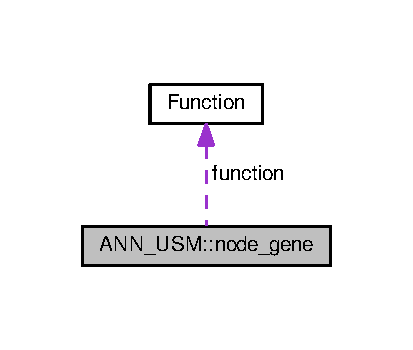
\includegraphics[width=198pt]{class_a_n_n___u_s_m_1_1node__gene__coll__graph}
\end{center}
\end{figure}
\subsection*{Public Member Functions}
\begin{DoxyCompactItemize}
\item 
\hyperlink{class_a_n_n___u_s_m_1_1node__gene_a2bd112df73cd91917c32456d7b74c19d}{node\-\_\-gene} ()
\item 
void \hyperlink{class_a_n_n___u_s_m_1_1node__gene_a96099b1c7cb2d302f802fd13080f65e1}{n\-\_\-g} (int \hyperlink{class_a_n_n___u_s_m_1_1node__gene_a426387db0b455d5e07debcf1ce186100}{node}, int \hyperlink{class_a_n_n___u_s_m_1_1node__gene_acf1e1356443a2ea954570d9e048ef72c}{row}, \hyperlink{namespace_a_n_n___u_s_m_aa7f97f486244dd898592ba14dd7aa778}{gene\-\_\-type} \hyperlink{class_a_n_n___u_s_m_1_1node__gene_abe075ac0849a7b7bb2aca6fac57cea00}{type}, string \hyperlink{class_a_n_n___u_s_m_1_1node__gene_a3191d2de9879934a6cd1331b2ffa68b8}{function})
\item 
void \hyperlink{class_a_n_n___u_s_m_1_1node__gene_a966ec45b4c692bf43244ae4fdc09a1c9}{kill} ()
\item 
void \hyperlink{class_a_n_n___u_s_m_1_1node__gene_ac9061b6f8289758f3b2f6a4fe27d0f88}{increase\-\_\-incoming\-\_\-connection} ()
\item 
void \hyperlink{class_a_n_n___u_s_m_1_1node__gene_a6fb9a8966511bc122c6fd12aa78ce9f8}{decrease\-\_\-incoming\-\_\-connection} ()
\item 
void \hyperlink{class_a_n_n___u_s_m_1_1node__gene_a50bf322d336d5783e74a6730f5854afa}{eval} (double value)
\item 
double \hyperlink{class_a_n_n___u_s_m_1_1node__gene_aa8261e2582b345e6202c8bcb88c45012}{get\-\_\-final\-\_\-result} ()
\item 
bool \hyperlink{class_a_n_n___u_s_m_1_1node__gene_a7b933ce737040d389da27d6569cb02f2}{is\-\_\-ready} ()
\end{DoxyCompactItemize}
\subsection*{Public Attributes}
\begin{DoxyCompactItemize}
\item 
int \hyperlink{class_a_n_n___u_s_m_1_1node__gene_acf1e1356443a2ea954570d9e048ef72c}{row}
\item 
int \hyperlink{class_a_n_n___u_s_m_1_1node__gene_a426387db0b455d5e07debcf1ce186100}{node}
\item 
int \hyperlink{class_a_n_n___u_s_m_1_1node__gene_a7e8526e6590c4cf1ee406246d952cc8a}{incoming\-\_\-connections}
\item 
int \hyperlink{class_a_n_n___u_s_m_1_1node__gene_a38eb3708558a74ce2ce8aac04c8511b8}{counter}
\item 
bool \hyperlink{class_a_n_n___u_s_m_1_1node__gene_a128ec887fd61121228a404b6c48f70ed}{exist}
\item 
double \hyperlink{class_a_n_n___u_s_m_1_1node__gene_a99515f1d21600249a72ab602cda1efdf}{accumulative\-\_\-result}
\item 
double \hyperlink{class_a_n_n___u_s_m_1_1node__gene_ab5311006a4d63b4eeed4b115d87c829a}{final\-\_\-result}
\item 
vector$<$ int $>$ \hyperlink{class_a_n_n___u_s_m_1_1node__gene_aa368c019e28b51deba3d01ecef5e85de}{outgoing\-\_\-connections}
\item 
\hyperlink{namespace_a_n_n___u_s_m_aa7f97f486244dd898592ba14dd7aa778}{gene\-\_\-type} \hyperlink{class_a_n_n___u_s_m_1_1node__gene_abe075ac0849a7b7bb2aca6fac57cea00}{type}
\item 
\hyperlink{class_function}{Function} $\ast$ \hyperlink{class_a_n_n___u_s_m_1_1node__gene_a3191d2de9879934a6cd1331b2ffa68b8}{function}
\end{DoxyCompactItemize}


\subsection{Detailed Description}


Definition at line 50 of file genetic\-\_\-encoding.\-hpp.



\subsection{Constructor \& Destructor Documentation}
\hypertarget{class_a_n_n___u_s_m_1_1node__gene_a2bd112df73cd91917c32456d7b74c19d}{\index{A\-N\-N\-\_\-\-U\-S\-M\-::node\-\_\-gene@{A\-N\-N\-\_\-\-U\-S\-M\-::node\-\_\-gene}!node\-\_\-gene@{node\-\_\-gene}}
\index{node\-\_\-gene@{node\-\_\-gene}!ANN_USM::node_gene@{A\-N\-N\-\_\-\-U\-S\-M\-::node\-\_\-gene}}
\subsubsection[{node\-\_\-gene}]{\setlength{\rightskip}{0pt plus 5cm}node\-\_\-gene\-::node\-\_\-gene (
\begin{DoxyParamCaption}
{}
\end{DoxyParamCaption}
)}}\label{class_a_n_n___u_s_m_1_1node__gene_a2bd112df73cd91917c32456d7b74c19d}


Definition at line 34 of file genetic\-\_\-encoding.\-cpp.



\subsection{Member Function Documentation}
\hypertarget{class_a_n_n___u_s_m_1_1node__gene_a6fb9a8966511bc122c6fd12aa78ce9f8}{\index{A\-N\-N\-\_\-\-U\-S\-M\-::node\-\_\-gene@{A\-N\-N\-\_\-\-U\-S\-M\-::node\-\_\-gene}!decrease\-\_\-incoming\-\_\-connection@{decrease\-\_\-incoming\-\_\-connection}}
\index{decrease\-\_\-incoming\-\_\-connection@{decrease\-\_\-incoming\-\_\-connection}!ANN_USM::node_gene@{A\-N\-N\-\_\-\-U\-S\-M\-::node\-\_\-gene}}
\subsubsection[{decrease\-\_\-incoming\-\_\-connection}]{\setlength{\rightskip}{0pt plus 5cm}void node\-\_\-gene\-::decrease\-\_\-incoming\-\_\-connection (
\begin{DoxyParamCaption}
{}
\end{DoxyParamCaption}
)}}\label{class_a_n_n___u_s_m_1_1node__gene_a6fb9a8966511bc122c6fd12aa78ce9f8}


Definition at line 71 of file genetic\-\_\-encoding.\-cpp.

\hypertarget{class_a_n_n___u_s_m_1_1node__gene_a50bf322d336d5783e74a6730f5854afa}{\index{A\-N\-N\-\_\-\-U\-S\-M\-::node\-\_\-gene@{A\-N\-N\-\_\-\-U\-S\-M\-::node\-\_\-gene}!eval@{eval}}
\index{eval@{eval}!ANN_USM::node_gene@{A\-N\-N\-\_\-\-U\-S\-M\-::node\-\_\-gene}}
\subsubsection[{eval}]{\setlength{\rightskip}{0pt plus 5cm}void node\-\_\-gene\-::eval (
\begin{DoxyParamCaption}
\item[{double}]{value}
\end{DoxyParamCaption}
)}}\label{class_a_n_n___u_s_m_1_1node__gene_a50bf322d336d5783e74a6730f5854afa}


Definition at line 76 of file genetic\-\_\-encoding.\-cpp.



Here is the call graph for this function\-:\nopagebreak
\begin{figure}[H]
\begin{center}
\leavevmode
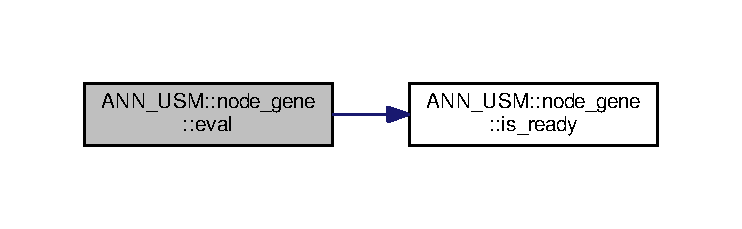
\includegraphics[width=350pt]{class_a_n_n___u_s_m_1_1node__gene_a50bf322d336d5783e74a6730f5854afa_cgraph}
\end{center}
\end{figure}


\hypertarget{class_a_n_n___u_s_m_1_1node__gene_aa8261e2582b345e6202c8bcb88c45012}{\index{A\-N\-N\-\_\-\-U\-S\-M\-::node\-\_\-gene@{A\-N\-N\-\_\-\-U\-S\-M\-::node\-\_\-gene}!get\-\_\-final\-\_\-result@{get\-\_\-final\-\_\-result}}
\index{get\-\_\-final\-\_\-result@{get\-\_\-final\-\_\-result}!ANN_USM::node_gene@{A\-N\-N\-\_\-\-U\-S\-M\-::node\-\_\-gene}}
\subsubsection[{get\-\_\-final\-\_\-result}]{\setlength{\rightskip}{0pt plus 5cm}double node\-\_\-gene\-::get\-\_\-final\-\_\-result (
\begin{DoxyParamCaption}
{}
\end{DoxyParamCaption}
)}}\label{class_a_n_n___u_s_m_1_1node__gene_aa8261e2582b345e6202c8bcb88c45012}


Definition at line 56 of file genetic\-\_\-encoding.\-cpp.

\hypertarget{class_a_n_n___u_s_m_1_1node__gene_ac9061b6f8289758f3b2f6a4fe27d0f88}{\index{A\-N\-N\-\_\-\-U\-S\-M\-::node\-\_\-gene@{A\-N\-N\-\_\-\-U\-S\-M\-::node\-\_\-gene}!increase\-\_\-incoming\-\_\-connection@{increase\-\_\-incoming\-\_\-connection}}
\index{increase\-\_\-incoming\-\_\-connection@{increase\-\_\-incoming\-\_\-connection}!ANN_USM::node_gene@{A\-N\-N\-\_\-\-U\-S\-M\-::node\-\_\-gene}}
\subsubsection[{increase\-\_\-incoming\-\_\-connection}]{\setlength{\rightskip}{0pt plus 5cm}void node\-\_\-gene\-::increase\-\_\-incoming\-\_\-connection (
\begin{DoxyParamCaption}
{}
\end{DoxyParamCaption}
)}}\label{class_a_n_n___u_s_m_1_1node__gene_ac9061b6f8289758f3b2f6a4fe27d0f88}


Definition at line 66 of file genetic\-\_\-encoding.\-cpp.

\hypertarget{class_a_n_n___u_s_m_1_1node__gene_a7b933ce737040d389da27d6569cb02f2}{\index{A\-N\-N\-\_\-\-U\-S\-M\-::node\-\_\-gene@{A\-N\-N\-\_\-\-U\-S\-M\-::node\-\_\-gene}!is\-\_\-ready@{is\-\_\-ready}}
\index{is\-\_\-ready@{is\-\_\-ready}!ANN_USM::node_gene@{A\-N\-N\-\_\-\-U\-S\-M\-::node\-\_\-gene}}
\subsubsection[{is\-\_\-ready}]{\setlength{\rightskip}{0pt plus 5cm}bool node\-\_\-gene\-::is\-\_\-ready (
\begin{DoxyParamCaption}
{}
\end{DoxyParamCaption}
)}}\label{class_a_n_n___u_s_m_1_1node__gene_a7b933ce737040d389da27d6569cb02f2}


Definition at line 61 of file genetic\-\_\-encoding.\-cpp.



Here is the caller graph for this function\-:\nopagebreak
\begin{figure}[H]
\begin{center}
\leavevmode
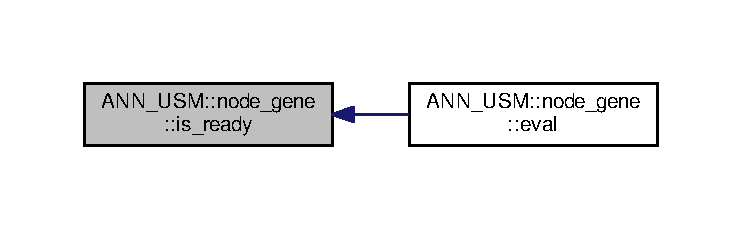
\includegraphics[width=350pt]{class_a_n_n___u_s_m_1_1node__gene_a7b933ce737040d389da27d6569cb02f2_icgraph}
\end{center}
\end{figure}


\hypertarget{class_a_n_n___u_s_m_1_1node__gene_a966ec45b4c692bf43244ae4fdc09a1c9}{\index{A\-N\-N\-\_\-\-U\-S\-M\-::node\-\_\-gene@{A\-N\-N\-\_\-\-U\-S\-M\-::node\-\_\-gene}!kill@{kill}}
\index{kill@{kill}!ANN_USM::node_gene@{A\-N\-N\-\_\-\-U\-S\-M\-::node\-\_\-gene}}
\subsubsection[{kill}]{\setlength{\rightskip}{0pt plus 5cm}void node\-\_\-gene\-::kill (
\begin{DoxyParamCaption}
{}
\end{DoxyParamCaption}
)}}\label{class_a_n_n___u_s_m_1_1node__gene_a966ec45b4c692bf43244ae4fdc09a1c9}


Definition at line 51 of file genetic\-\_\-encoding.\-cpp.



Here is the caller graph for this function\-:\nopagebreak
\begin{figure}[H]
\begin{center}
\leavevmode
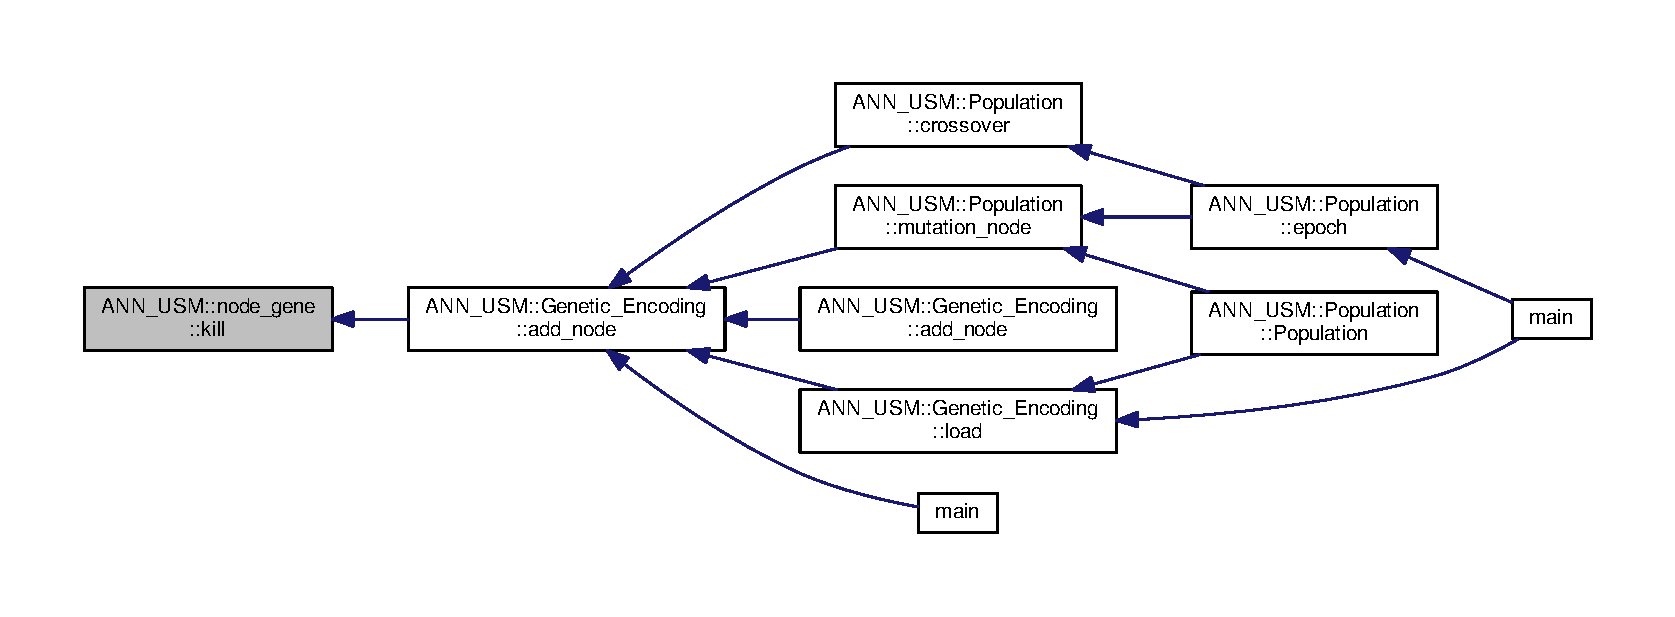
\includegraphics[width=350pt]{class_a_n_n___u_s_m_1_1node__gene_a966ec45b4c692bf43244ae4fdc09a1c9_icgraph}
\end{center}
\end{figure}


\hypertarget{class_a_n_n___u_s_m_1_1node__gene_a96099b1c7cb2d302f802fd13080f65e1}{\index{A\-N\-N\-\_\-\-U\-S\-M\-::node\-\_\-gene@{A\-N\-N\-\_\-\-U\-S\-M\-::node\-\_\-gene}!n\-\_\-g@{n\-\_\-g}}
\index{n\-\_\-g@{n\-\_\-g}!ANN_USM::node_gene@{A\-N\-N\-\_\-\-U\-S\-M\-::node\-\_\-gene}}
\subsubsection[{n\-\_\-g}]{\setlength{\rightskip}{0pt plus 5cm}void node\-\_\-gene\-::n\-\_\-g (
\begin{DoxyParamCaption}
\item[{int}]{node, }
\item[{int}]{row, }
\item[{{\bf gene\-\_\-type}}]{type, }
\item[{string}]{function}
\end{DoxyParamCaption}
)}}\label{class_a_n_n___u_s_m_1_1node__gene_a96099b1c7cb2d302f802fd13080f65e1}


Definition at line 42 of file genetic\-\_\-encoding.\-cpp.



Here is the caller graph for this function\-:\nopagebreak
\begin{figure}[H]
\begin{center}
\leavevmode
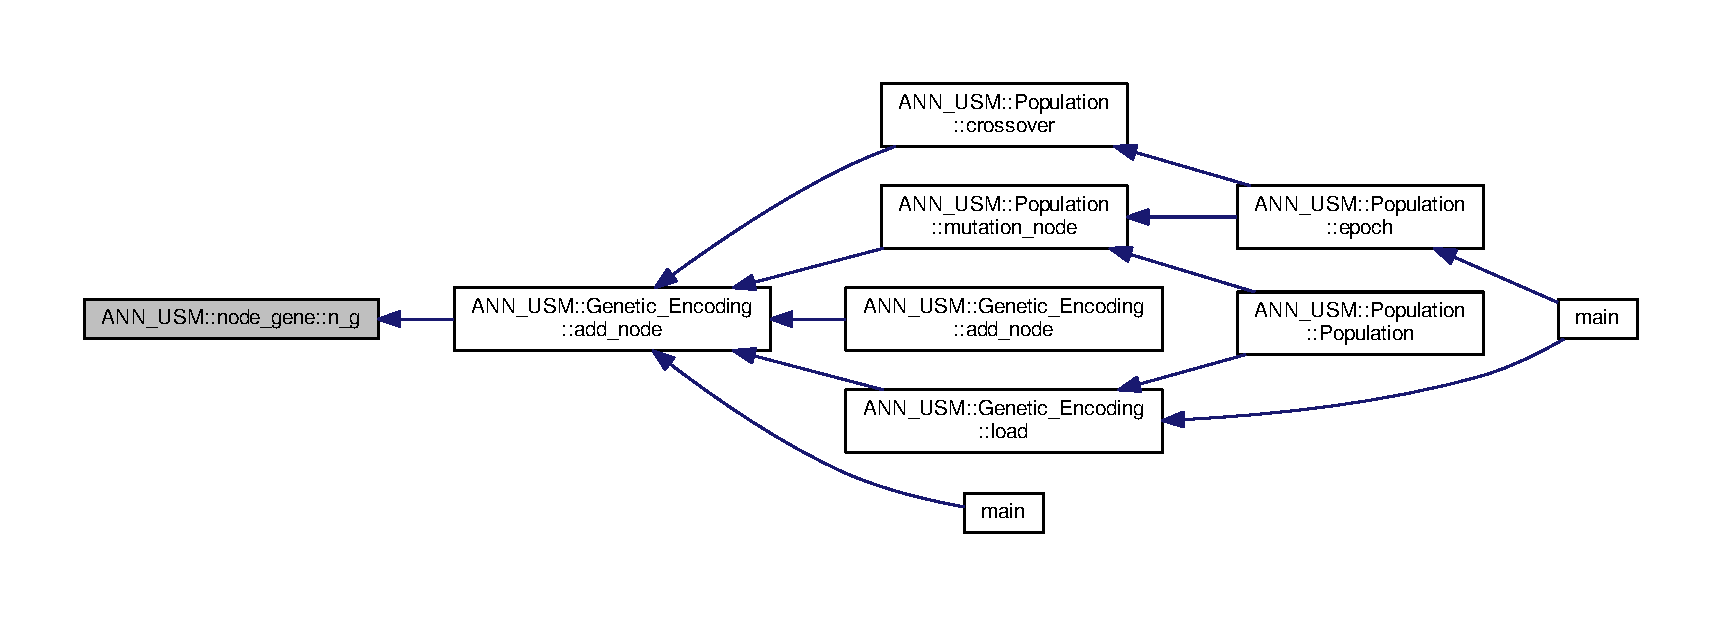
\includegraphics[width=350pt]{class_a_n_n___u_s_m_1_1node__gene_a96099b1c7cb2d302f802fd13080f65e1_icgraph}
\end{center}
\end{figure}




\subsection{Member Data Documentation}
\hypertarget{class_a_n_n___u_s_m_1_1node__gene_a99515f1d21600249a72ab602cda1efdf}{\index{A\-N\-N\-\_\-\-U\-S\-M\-::node\-\_\-gene@{A\-N\-N\-\_\-\-U\-S\-M\-::node\-\_\-gene}!accumulative\-\_\-result@{accumulative\-\_\-result}}
\index{accumulative\-\_\-result@{accumulative\-\_\-result}!ANN_USM::node_gene@{A\-N\-N\-\_\-\-U\-S\-M\-::node\-\_\-gene}}
\subsubsection[{accumulative\-\_\-result}]{\setlength{\rightskip}{0pt plus 5cm}double A\-N\-N\-\_\-\-U\-S\-M\-::node\-\_\-gene\-::accumulative\-\_\-result}}\label{class_a_n_n___u_s_m_1_1node__gene_a99515f1d21600249a72ab602cda1efdf}


Definition at line 73 of file genetic\-\_\-encoding.\-hpp.

\hypertarget{class_a_n_n___u_s_m_1_1node__gene_a38eb3708558a74ce2ce8aac04c8511b8}{\index{A\-N\-N\-\_\-\-U\-S\-M\-::node\-\_\-gene@{A\-N\-N\-\_\-\-U\-S\-M\-::node\-\_\-gene}!counter@{counter}}
\index{counter@{counter}!ANN_USM::node_gene@{A\-N\-N\-\_\-\-U\-S\-M\-::node\-\_\-gene}}
\subsubsection[{counter}]{\setlength{\rightskip}{0pt plus 5cm}int A\-N\-N\-\_\-\-U\-S\-M\-::node\-\_\-gene\-::counter}}\label{class_a_n_n___u_s_m_1_1node__gene_a38eb3708558a74ce2ce8aac04c8511b8}


Definition at line 69 of file genetic\-\_\-encoding.\-hpp.

\hypertarget{class_a_n_n___u_s_m_1_1node__gene_a128ec887fd61121228a404b6c48f70ed}{\index{A\-N\-N\-\_\-\-U\-S\-M\-::node\-\_\-gene@{A\-N\-N\-\_\-\-U\-S\-M\-::node\-\_\-gene}!exist@{exist}}
\index{exist@{exist}!ANN_USM::node_gene@{A\-N\-N\-\_\-\-U\-S\-M\-::node\-\_\-gene}}
\subsubsection[{exist}]{\setlength{\rightskip}{0pt plus 5cm}bool A\-N\-N\-\_\-\-U\-S\-M\-::node\-\_\-gene\-::exist}}\label{class_a_n_n___u_s_m_1_1node__gene_a128ec887fd61121228a404b6c48f70ed}


Definition at line 71 of file genetic\-\_\-encoding.\-hpp.

\hypertarget{class_a_n_n___u_s_m_1_1node__gene_ab5311006a4d63b4eeed4b115d87c829a}{\index{A\-N\-N\-\_\-\-U\-S\-M\-::node\-\_\-gene@{A\-N\-N\-\_\-\-U\-S\-M\-::node\-\_\-gene}!final\-\_\-result@{final\-\_\-result}}
\index{final\-\_\-result@{final\-\_\-result}!ANN_USM::node_gene@{A\-N\-N\-\_\-\-U\-S\-M\-::node\-\_\-gene}}
\subsubsection[{final\-\_\-result}]{\setlength{\rightskip}{0pt plus 5cm}double A\-N\-N\-\_\-\-U\-S\-M\-::node\-\_\-gene\-::final\-\_\-result}}\label{class_a_n_n___u_s_m_1_1node__gene_ab5311006a4d63b4eeed4b115d87c829a}


Definition at line 74 of file genetic\-\_\-encoding.\-hpp.

\hypertarget{class_a_n_n___u_s_m_1_1node__gene_a3191d2de9879934a6cd1331b2ffa68b8}{\index{A\-N\-N\-\_\-\-U\-S\-M\-::node\-\_\-gene@{A\-N\-N\-\_\-\-U\-S\-M\-::node\-\_\-gene}!function@{function}}
\index{function@{function}!ANN_USM::node_gene@{A\-N\-N\-\_\-\-U\-S\-M\-::node\-\_\-gene}}
\subsubsection[{function}]{\setlength{\rightskip}{0pt plus 5cm}{\bf Function}$\ast$ A\-N\-N\-\_\-\-U\-S\-M\-::node\-\_\-gene\-::function}}\label{class_a_n_n___u_s_m_1_1node__gene_a3191d2de9879934a6cd1331b2ffa68b8}


Definition at line 81 of file genetic\-\_\-encoding.\-hpp.

\hypertarget{class_a_n_n___u_s_m_1_1node__gene_a7e8526e6590c4cf1ee406246d952cc8a}{\index{A\-N\-N\-\_\-\-U\-S\-M\-::node\-\_\-gene@{A\-N\-N\-\_\-\-U\-S\-M\-::node\-\_\-gene}!incoming\-\_\-connections@{incoming\-\_\-connections}}
\index{incoming\-\_\-connections@{incoming\-\_\-connections}!ANN_USM::node_gene@{A\-N\-N\-\_\-\-U\-S\-M\-::node\-\_\-gene}}
\subsubsection[{incoming\-\_\-connections}]{\setlength{\rightskip}{0pt plus 5cm}int A\-N\-N\-\_\-\-U\-S\-M\-::node\-\_\-gene\-::incoming\-\_\-connections}}\label{class_a_n_n___u_s_m_1_1node__gene_a7e8526e6590c4cf1ee406246d952cc8a}


Definition at line 68 of file genetic\-\_\-encoding.\-hpp.

\hypertarget{class_a_n_n___u_s_m_1_1node__gene_a426387db0b455d5e07debcf1ce186100}{\index{A\-N\-N\-\_\-\-U\-S\-M\-::node\-\_\-gene@{A\-N\-N\-\_\-\-U\-S\-M\-::node\-\_\-gene}!node@{node}}
\index{node@{node}!ANN_USM::node_gene@{A\-N\-N\-\_\-\-U\-S\-M\-::node\-\_\-gene}}
\subsubsection[{node}]{\setlength{\rightskip}{0pt plus 5cm}int A\-N\-N\-\_\-\-U\-S\-M\-::node\-\_\-gene\-::node}}\label{class_a_n_n___u_s_m_1_1node__gene_a426387db0b455d5e07debcf1ce186100}


Definition at line 67 of file genetic\-\_\-encoding.\-hpp.

\hypertarget{class_a_n_n___u_s_m_1_1node__gene_aa368c019e28b51deba3d01ecef5e85de}{\index{A\-N\-N\-\_\-\-U\-S\-M\-::node\-\_\-gene@{A\-N\-N\-\_\-\-U\-S\-M\-::node\-\_\-gene}!outgoing\-\_\-connections@{outgoing\-\_\-connections}}
\index{outgoing\-\_\-connections@{outgoing\-\_\-connections}!ANN_USM::node_gene@{A\-N\-N\-\_\-\-U\-S\-M\-::node\-\_\-gene}}
\subsubsection[{outgoing\-\_\-connections}]{\setlength{\rightskip}{0pt plus 5cm}vector$<$int$>$ A\-N\-N\-\_\-\-U\-S\-M\-::node\-\_\-gene\-::outgoing\-\_\-connections}}\label{class_a_n_n___u_s_m_1_1node__gene_aa368c019e28b51deba3d01ecef5e85de}


Definition at line 77 of file genetic\-\_\-encoding.\-hpp.

\hypertarget{class_a_n_n___u_s_m_1_1node__gene_acf1e1356443a2ea954570d9e048ef72c}{\index{A\-N\-N\-\_\-\-U\-S\-M\-::node\-\_\-gene@{A\-N\-N\-\_\-\-U\-S\-M\-::node\-\_\-gene}!row@{row}}
\index{row@{row}!ANN_USM::node_gene@{A\-N\-N\-\_\-\-U\-S\-M\-::node\-\_\-gene}}
\subsubsection[{row}]{\setlength{\rightskip}{0pt plus 5cm}int A\-N\-N\-\_\-\-U\-S\-M\-::node\-\_\-gene\-::row}}\label{class_a_n_n___u_s_m_1_1node__gene_acf1e1356443a2ea954570d9e048ef72c}


Definition at line 66 of file genetic\-\_\-encoding.\-hpp.

\hypertarget{class_a_n_n___u_s_m_1_1node__gene_abe075ac0849a7b7bb2aca6fac57cea00}{\index{A\-N\-N\-\_\-\-U\-S\-M\-::node\-\_\-gene@{A\-N\-N\-\_\-\-U\-S\-M\-::node\-\_\-gene}!type@{type}}
\index{type@{type}!ANN_USM::node_gene@{A\-N\-N\-\_\-\-U\-S\-M\-::node\-\_\-gene}}
\subsubsection[{type}]{\setlength{\rightskip}{0pt plus 5cm}{\bf gene\-\_\-type} A\-N\-N\-\_\-\-U\-S\-M\-::node\-\_\-gene\-::type}}\label{class_a_n_n___u_s_m_1_1node__gene_abe075ac0849a7b7bb2aca6fac57cea00}


Definition at line 79 of file genetic\-\_\-encoding.\-hpp.



The documentation for this class was generated from the following files\-:\begin{DoxyCompactItemize}
\item 
headers/\hyperlink{genetic__encoding_8hpp}{genetic\-\_\-encoding.\-hpp}\item 
src/\hyperlink{genetic__encoding_8cpp}{genetic\-\_\-encoding.\-cpp}\end{DoxyCompactItemize}

\hypertarget{class_a_n_n___u_s_m_1_1_population}{\section{A\-N\-N\-\_\-\-U\-S\-M\-:\-:Population Class Reference}
\label{class_a_n_n___u_s_m_1_1_population}\index{A\-N\-N\-\_\-\-U\-S\-M\-::\-Population@{A\-N\-N\-\_\-\-U\-S\-M\-::\-Population}}
}


{\ttfamily \#include $<$C\-P\-P\-N-\/\-N\-E\-A\-T.\-hpp$>$}



Collaboration diagram for A\-N\-N\-\_\-\-U\-S\-M\-:\-:Population\-:\nopagebreak
\begin{figure}[H]
\begin{center}
\leavevmode
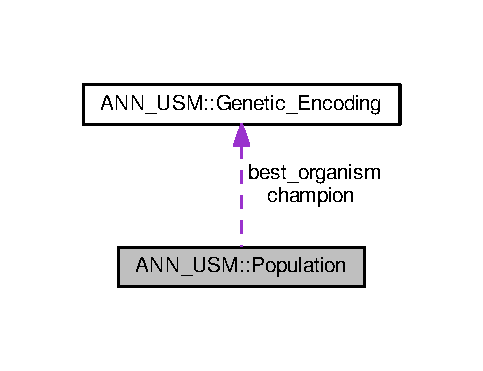
\includegraphics[width=232pt]{class_a_n_n___u_s_m_1_1_population__coll__graph}
\end{center}
\end{figure}
\subsection*{Public Member Functions}
\begin{DoxyCompactItemize}
\item 
\hyperlink{class_a_n_n___u_s_m_1_1_population_a9c5a7b47b6fa36d3c53788029c33bd98}{Population} (char path\mbox{[}$\,$\mbox{]})
\item 
void \hyperlink{class_a_n_n___u_s_m_1_1_population_af15b09e6b9ca34cf5c7f15fe33d1c5bb}{save\-\_\-all} (char path\mbox{[}$\,$\mbox{]})
\item 
void \hyperlink{class_a_n_n___u_s_m_1_1_population_ad6a8d08fc4f4cbcc84405ddd7e40a453}{save} (char path\mbox{[}$\,$\mbox{]})
\item 
void \hyperlink{class_a_n_n___u_s_m_1_1_population_afcedc0302e1ce8e399f5ffb914ed216c}{epoch} ()
\item 
void \hyperlink{class_a_n_n___u_s_m_1_1_population_aa14d8cb45306aa8b9851791a6d547be6}{spatiation} ()
\item 
int \hyperlink{class_a_n_n___u_s_m_1_1_population_a037c144dd6c90391d312a1b38af6e057}{obtain\-\_\-historical\-\_\-node} (int initial\-\_\-in, int initial\-\_\-out)
\item 
int \hyperlink{class_a_n_n___u_s_m_1_1_population_a16090fdb0f1e89cc91568028777ac847}{obtain\-\_\-innovation} (int in, int out)
\begin{DoxyCompactList}\small\item\em Obtain the (historical) innovation number between two nodes. \end{DoxyCompactList}\item 
int \hyperlink{class_a_n_n___u_s_m_1_1_population_a84ab90f06fe08ed2b95638427086a331}{obtain\-\_\-row} (int node, int node\-\_\-initial\-\_\-in, int node\-\_\-initial\-\_\-out)
\item 
double \hyperlink{class_a_n_n___u_s_m_1_1_population_a92308bf99765cb66506c3ac4c1ee227c}{compatibility} (\hyperlink{class_a_n_n___u_s_m_1_1_genetic___encoding}{Genetic\-\_\-\-Encoding} orgm1, \hyperlink{class_a_n_n___u_s_m_1_1_genetic___encoding}{Genetic\-\_\-\-Encoding} orgm2)
\begin{DoxyCompactList}\small\item\em Measure the distance between two organism. \end{DoxyCompactList}\item 
\hyperlink{class_a_n_n___u_s_m_1_1_genetic___encoding}{Genetic\-\_\-\-Encoding} \hyperlink{class_a_n_n___u_s_m_1_1_population_a20ca394c0565450c1843333129057027}{mutation\-\_\-node} (\hyperlink{class_a_n_n___u_s_m_1_1_genetic___encoding}{Genetic\-\_\-\-Encoding} organism)
\item 
\hyperlink{class_a_n_n___u_s_m_1_1_genetic___encoding}{Genetic\-\_\-\-Encoding} \hyperlink{class_a_n_n___u_s_m_1_1_population_acee4c5ba8e56deb1386864d349d78316}{mutation\-\_\-connection} (\hyperlink{class_a_n_n___u_s_m_1_1_genetic___encoding}{Genetic\-\_\-\-Encoding} organism)
\item 
\hyperlink{class_a_n_n___u_s_m_1_1_genetic___encoding}{Genetic\-\_\-\-Encoding} \hyperlink{class_a_n_n___u_s_m_1_1_population_aae7b2c347f1e8fbe0165e4d6f839a277}{mutation\-\_\-change\-\_\-weight} (\hyperlink{class_a_n_n___u_s_m_1_1_genetic___encoding}{Genetic\-\_\-\-Encoding} organism)
\item 
\hyperlink{class_a_n_n___u_s_m_1_1_genetic___encoding}{Genetic\-\_\-\-Encoding} \hyperlink{class_a_n_n___u_s_m_1_1_population_a0b858ba5af6628979fd7f136520cdd5b}{put\-\_\-randoms\-\_\-weight} (\hyperlink{class_a_n_n___u_s_m_1_1_genetic___encoding}{Genetic\-\_\-\-Encoding} organism)
\item 
\hyperlink{class_a_n_n___u_s_m_1_1_genetic___encoding}{Genetic\-\_\-\-Encoding} \hyperlink{class_a_n_n___u_s_m_1_1_population_a026d44aeb16651486c78dd8c8e0a293d}{crossover} (\hyperlink{class_a_n_n___u_s_m_1_1_genetic___encoding}{Genetic\-\_\-\-Encoding} orgm1, \hyperlink{class_a_n_n___u_s_m_1_1_genetic___encoding}{Genetic\-\_\-\-Encoding} orgm2)
\end{DoxyCompactItemize}
\subsection*{Public Attributes}
\begin{DoxyCompactItemize}
\item 
int \hyperlink{class_a_n_n___u_s_m_1_1_population_a9a9980d69d2a013d4dfc1388b7d96db6}{lenght}
\item 
int \hyperlink{class_a_n_n___u_s_m_1_1_population_a5dd00b369c21214466d0f155ba0e11ee}{total\-\_\-niches}
\item 
int \hyperlink{class_a_n_n___u_s_m_1_1_population_a609df33a9f9f1221ddf5604ef01dace5}{last\-\_\-niche\-\_\-id}
\item 
int \hyperlink{class_a_n_n___u_s_m_1_1_population_a836ae3c612ff56cac400ddea08893961}{last\-\_\-innovation}
\item 
int \hyperlink{class_a_n_n___u_s_m_1_1_population_a2c53f59115f21a4b42e91f8aca35cdcf}{last\-\_\-node}
\item 
int \hyperlink{class_a_n_n___u_s_m_1_1_population_a158d58cd6154506562b3a4b4cc563034}{last\-\_\-row}
\item 
double \hyperlink{class_a_n_n___u_s_m_1_1_population_a0622623a426583853cd7cc1e16bd9423}{fitness\-\_\-champion}
\item 
vector$<$ \hyperlink{class_a_n_n___u_s_m_1_1_genetic___encoding}{Genetic\-\_\-\-Encoding} $>$ \hyperlink{class_a_n_n___u_s_m_1_1_population_a98468ee8221857cad41ae4d7b2ae01cf}{organisms}
\item 
vector$<$ \hyperlink{class_a_n_n___u_s_m_1_1_genetic___encoding}{Genetic\-\_\-\-Encoding} $>$ \hyperlink{class_a_n_n___u_s_m_1_1_population_ad1ba3ace7157e2763976a1ee1155584b}{prev\-\_\-organisms}
\item 
vector$<$ \hyperlink{class_a_n_n___u_s_m_1_1_niche}{Niche} $>$ \hyperlink{class_a_n_n___u_s_m_1_1_population_aa45357359720f5ce88603d0282d22f17}{current\-\_\-niches}
\item 
vector$<$ \hyperlink{class_a_n_n___u_s_m_1_1_niche}{Niche} $>$ \hyperlink{class_a_n_n___u_s_m_1_1_population_a1103c56991771d6ccae5e1cccaf51db9}{prev\-\_\-niches}
\item 
\hyperlink{class_a_n_n___u_s_m_1_1_genetic___encoding}{Genetic\-\_\-\-Encoding} $\ast$ \hyperlink{class_a_n_n___u_s_m_1_1_population_a00cc470bf44ddbb9c104d3eead923dc3}{best\-\_\-organism}
\item 
\hyperlink{class_a_n_n___u_s_m_1_1_genetic___encoding}{Genetic\-\_\-\-Encoding} \hyperlink{class_a_n_n___u_s_m_1_1_population_a8fadd74c69061f51a5e3ea9a3d4aa516}{champion}
\item 
vector$<$ vector$<$ int $>$ $>$ \hyperlink{class_a_n_n___u_s_m_1_1_population_a5cbc92463b8bf0cc1031441ecfcd16bf}{historical\-\_\-nodes}
\item 
vector$<$ vector$<$ int $>$ $>$ \hyperlink{class_a_n_n___u_s_m_1_1_population_a980dc824cafc3dd2750f87c3300cdb95}{historical\-\_\-innovation}
\item 
vector$<$ int $>$ \hyperlink{class_a_n_n___u_s_m_1_1_population_ad2643c1369c231da3de9878dfaa0ccf2}{historical\-\_\-row}
\item 
vector$<$ int $>$ \hyperlink{class_a_n_n___u_s_m_1_1_population_ae688b66299b4b8be34d34a797bbc44ab}{row\-\_\-orderer\-\_\-list}
\end{DoxyCompactItemize}


\subsection{Detailed Description}


Definition at line 37 of file C\-P\-P\-N-\/\-N\-E\-A\-T.\-hpp.



\subsection{Constructor \& Destructor Documentation}
\hypertarget{class_a_n_n___u_s_m_1_1_population_a9c5a7b47b6fa36d3c53788029c33bd98}{\index{A\-N\-N\-\_\-\-U\-S\-M\-::\-Population@{A\-N\-N\-\_\-\-U\-S\-M\-::\-Population}!Population@{Population}}
\index{Population@{Population}!ANN_USM::Population@{A\-N\-N\-\_\-\-U\-S\-M\-::\-Population}}
\subsubsection[{Population}]{\setlength{\rightskip}{0pt plus 5cm}Population\-::\-Population (
\begin{DoxyParamCaption}
\item[{char}]{path\mbox{[}$\,$\mbox{]}}
\end{DoxyParamCaption}
)}}\label{class_a_n_n___u_s_m_1_1_population_a9c5a7b47b6fa36d3c53788029c33bd98}


Definition at line 13 of file C\-P\-P\-N-\/\-N\-E\-A\-T.\-cpp.



Here is the call graph for this function\-:\nopagebreak
\begin{figure}[H]
\begin{center}
\leavevmode
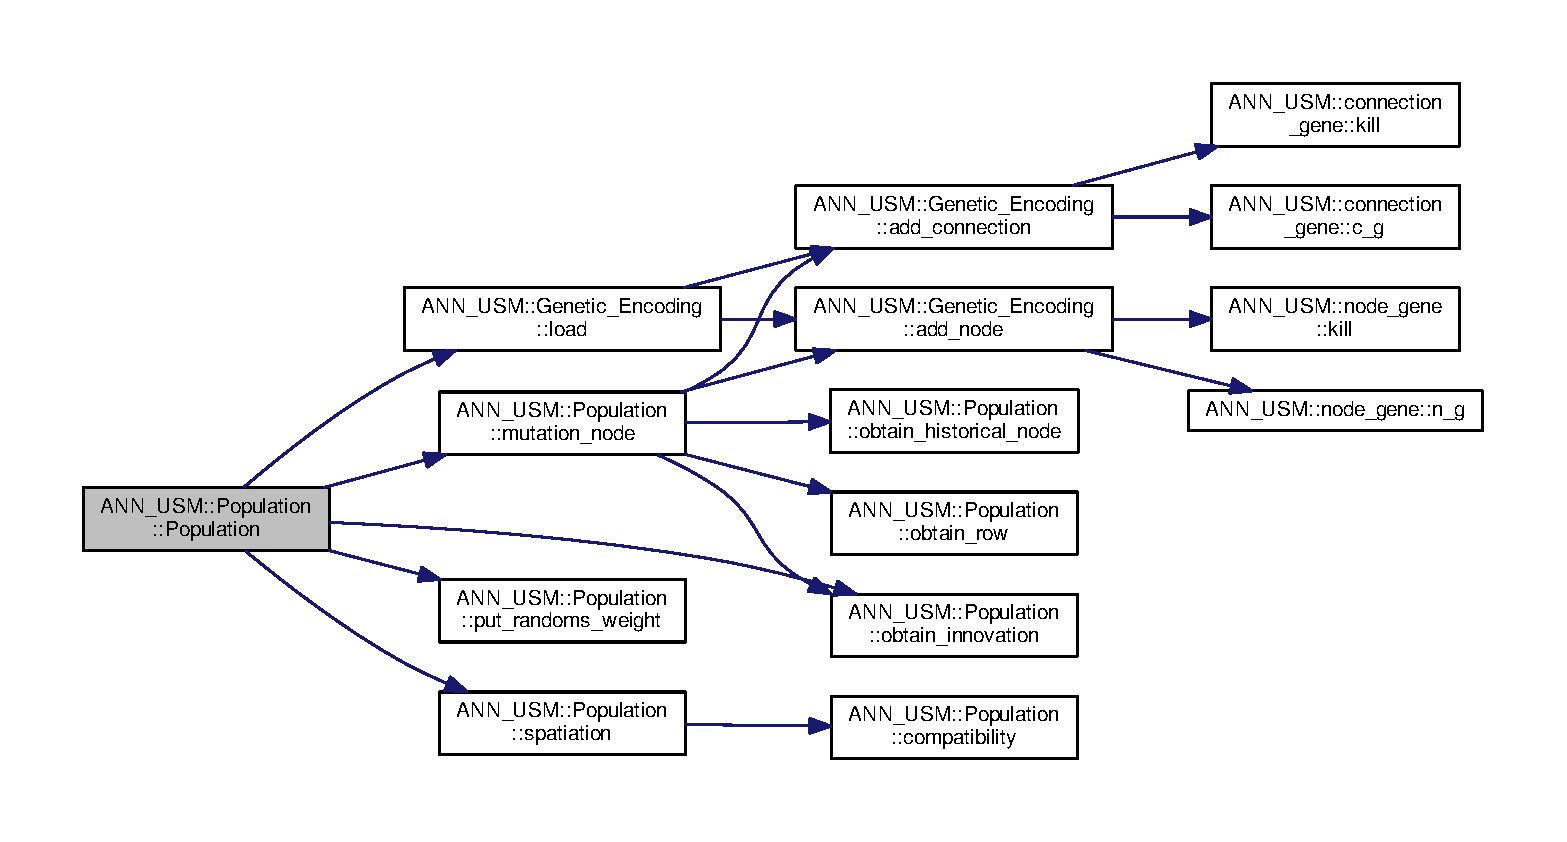
\includegraphics[width=350pt]{class_a_n_n___u_s_m_1_1_population_a9c5a7b47b6fa36d3c53788029c33bd98_cgraph}
\end{center}
\end{figure}




\subsection{Member Function Documentation}
\hypertarget{class_a_n_n___u_s_m_1_1_population_a92308bf99765cb66506c3ac4c1ee227c}{\index{A\-N\-N\-\_\-\-U\-S\-M\-::\-Population@{A\-N\-N\-\_\-\-U\-S\-M\-::\-Population}!compatibility@{compatibility}}
\index{compatibility@{compatibility}!ANN_USM::Population@{A\-N\-N\-\_\-\-U\-S\-M\-::\-Population}}
\subsubsection[{compatibility}]{\setlength{\rightskip}{0pt plus 5cm}double Population\-::compatibility (
\begin{DoxyParamCaption}
\item[{{\bf Genetic\-\_\-\-Encoding}}]{orgm1, }
\item[{{\bf Genetic\-\_\-\-Encoding}}]{orgm2}
\end{DoxyParamCaption}
)}}\label{class_a_n_n___u_s_m_1_1_population_a92308bf99765cb66506c3ac4c1ee227c}


Measure the distance between two organism. 



Definition at line 341 of file C\-P\-P\-N-\/\-N\-E\-A\-T.\-cpp.



Here is the caller graph for this function\-:\nopagebreak
\begin{figure}[H]
\begin{center}
\leavevmode
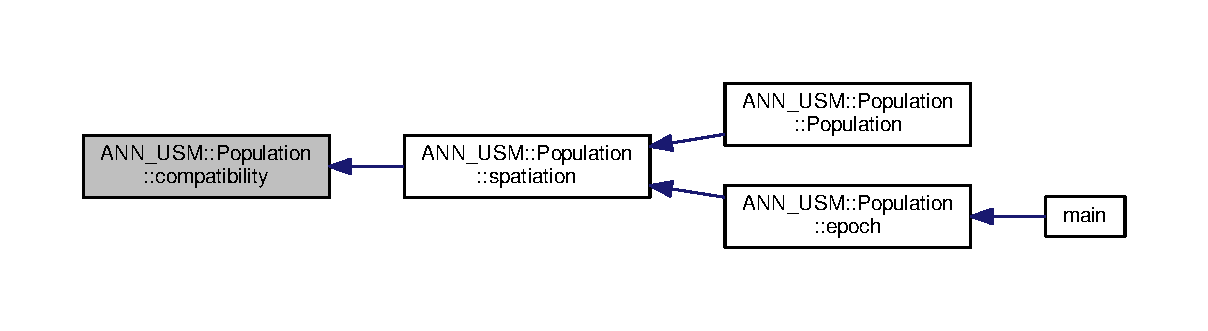
\includegraphics[width=350pt]{class_a_n_n___u_s_m_1_1_population_a92308bf99765cb66506c3ac4c1ee227c_icgraph}
\end{center}
\end{figure}


\hypertarget{class_a_n_n___u_s_m_1_1_population_a026d44aeb16651486c78dd8c8e0a293d}{\index{A\-N\-N\-\_\-\-U\-S\-M\-::\-Population@{A\-N\-N\-\_\-\-U\-S\-M\-::\-Population}!crossover@{crossover}}
\index{crossover@{crossover}!ANN_USM::Population@{A\-N\-N\-\_\-\-U\-S\-M\-::\-Population}}
\subsubsection[{crossover}]{\setlength{\rightskip}{0pt plus 5cm}{\bf Genetic\-\_\-\-Encoding} Population\-::crossover (
\begin{DoxyParamCaption}
\item[{{\bf Genetic\-\_\-\-Encoding}}]{orgm1, }
\item[{{\bf Genetic\-\_\-\-Encoding}}]{orgm2}
\end{DoxyParamCaption}
)}}\label{class_a_n_n___u_s_m_1_1_population_a026d44aeb16651486c78dd8c8e0a293d}


Definition at line 370 of file C\-P\-P\-N-\/\-N\-E\-A\-T.\-cpp.



Here is the call graph for this function\-:\nopagebreak
\begin{figure}[H]
\begin{center}
\leavevmode
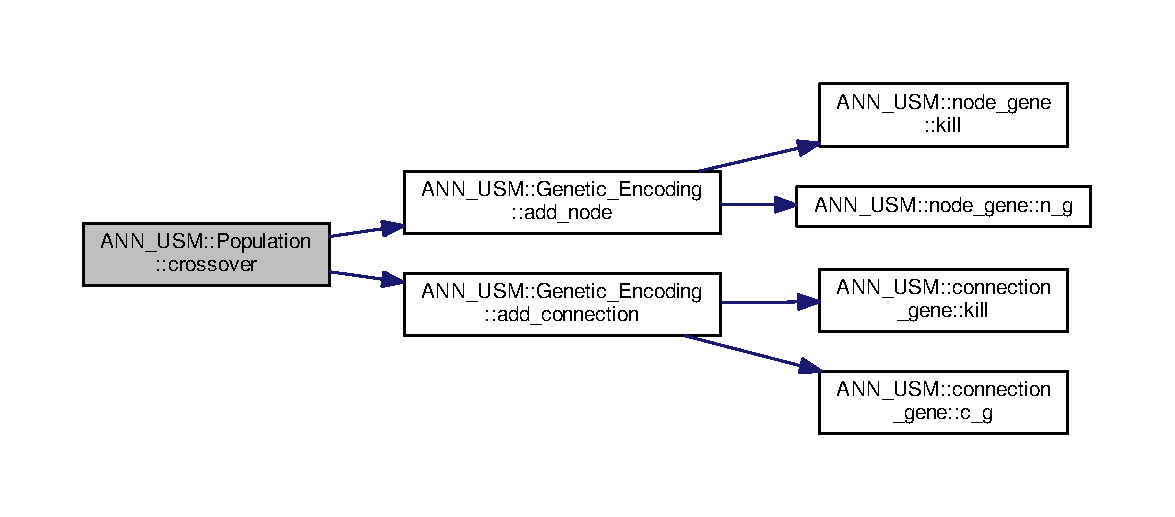
\includegraphics[width=350pt]{class_a_n_n___u_s_m_1_1_population_a026d44aeb16651486c78dd8c8e0a293d_cgraph}
\end{center}
\end{figure}




Here is the caller graph for this function\-:\nopagebreak
\begin{figure}[H]
\begin{center}
\leavevmode
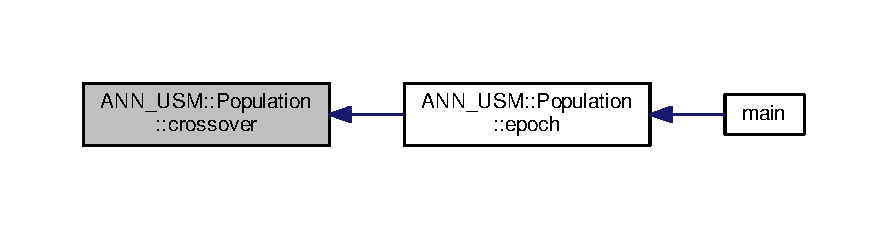
\includegraphics[width=350pt]{class_a_n_n___u_s_m_1_1_population_a026d44aeb16651486c78dd8c8e0a293d_icgraph}
\end{center}
\end{figure}


\hypertarget{class_a_n_n___u_s_m_1_1_population_afcedc0302e1ce8e399f5ffb914ed216c}{\index{A\-N\-N\-\_\-\-U\-S\-M\-::\-Population@{A\-N\-N\-\_\-\-U\-S\-M\-::\-Population}!epoch@{epoch}}
\index{epoch@{epoch}!ANN_USM::Population@{A\-N\-N\-\_\-\-U\-S\-M\-::\-Population}}
\subsubsection[{epoch}]{\setlength{\rightskip}{0pt plus 5cm}void Population\-::epoch (
\begin{DoxyParamCaption}
{}
\end{DoxyParamCaption}
)}}\label{class_a_n_n___u_s_m_1_1_population_afcedc0302e1ce8e399f5ffb914ed216c}


Definition at line 530 of file C\-P\-P\-N-\/\-N\-E\-A\-T.\-cpp.



Here is the call graph for this function\-:\nopagebreak
\begin{figure}[H]
\begin{center}
\leavevmode
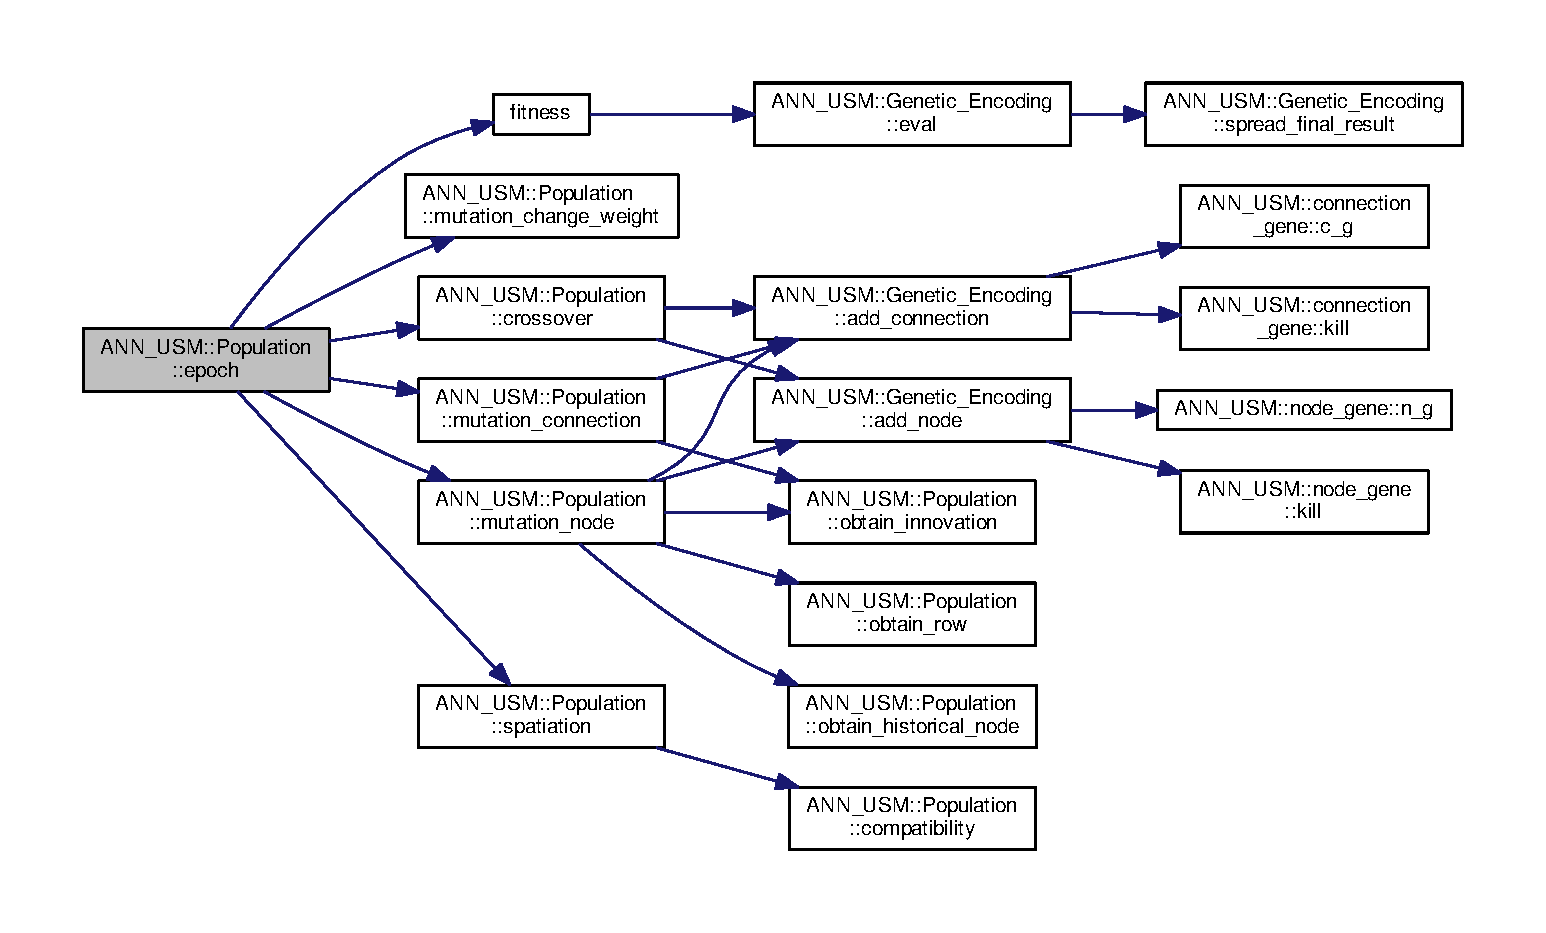
\includegraphics[width=350pt]{class_a_n_n___u_s_m_1_1_population_afcedc0302e1ce8e399f5ffb914ed216c_cgraph}
\end{center}
\end{figure}




Here is the caller graph for this function\-:\nopagebreak
\begin{figure}[H]
\begin{center}
\leavevmode
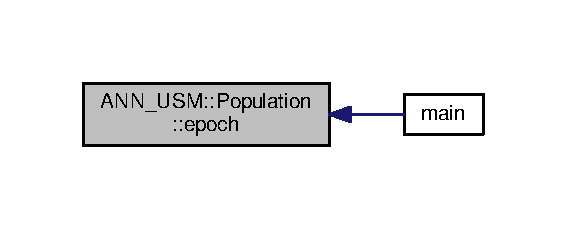
\includegraphics[width=272pt]{class_a_n_n___u_s_m_1_1_population_afcedc0302e1ce8e399f5ffb914ed216c_icgraph}
\end{center}
\end{figure}


\hypertarget{class_a_n_n___u_s_m_1_1_population_aae7b2c347f1e8fbe0165e4d6f839a277}{\index{A\-N\-N\-\_\-\-U\-S\-M\-::\-Population@{A\-N\-N\-\_\-\-U\-S\-M\-::\-Population}!mutation\-\_\-change\-\_\-weight@{mutation\-\_\-change\-\_\-weight}}
\index{mutation\-\_\-change\-\_\-weight@{mutation\-\_\-change\-\_\-weight}!ANN_USM::Population@{A\-N\-N\-\_\-\-U\-S\-M\-::\-Population}}
\subsubsection[{mutation\-\_\-change\-\_\-weight}]{\setlength{\rightskip}{0pt plus 5cm}{\bf Genetic\-\_\-\-Encoding} Population\-::mutation\-\_\-change\-\_\-weight (
\begin{DoxyParamCaption}
\item[{{\bf Genetic\-\_\-\-Encoding}}]{organism}
\end{DoxyParamCaption}
)}}\label{class_a_n_n___u_s_m_1_1_population_aae7b2c347f1e8fbe0165e4d6f839a277}


Definition at line 57 of file C\-P\-P\-N-\/\-N\-E\-A\-T.\-cpp.



Here is the caller graph for this function\-:\nopagebreak
\begin{figure}[H]
\begin{center}
\leavevmode
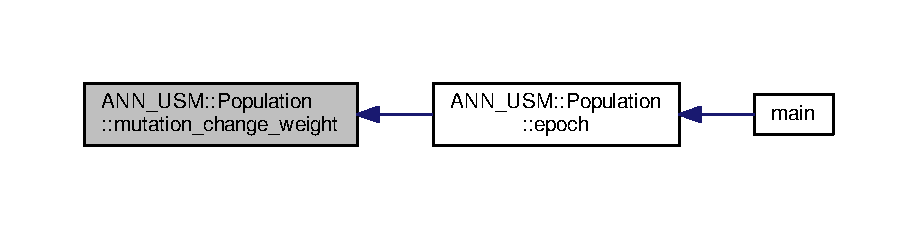
\includegraphics[width=350pt]{class_a_n_n___u_s_m_1_1_population_aae7b2c347f1e8fbe0165e4d6f839a277_icgraph}
\end{center}
\end{figure}


\hypertarget{class_a_n_n___u_s_m_1_1_population_acee4c5ba8e56deb1386864d349d78316}{\index{A\-N\-N\-\_\-\-U\-S\-M\-::\-Population@{A\-N\-N\-\_\-\-U\-S\-M\-::\-Population}!mutation\-\_\-connection@{mutation\-\_\-connection}}
\index{mutation\-\_\-connection@{mutation\-\_\-connection}!ANN_USM::Population@{A\-N\-N\-\_\-\-U\-S\-M\-::\-Population}}
\subsubsection[{mutation\-\_\-connection}]{\setlength{\rightskip}{0pt plus 5cm}{\bf Genetic\-\_\-\-Encoding} Population\-::mutation\-\_\-connection (
\begin{DoxyParamCaption}
\item[{{\bf Genetic\-\_\-\-Encoding}}]{organism}
\end{DoxyParamCaption}
)}}\label{class_a_n_n___u_s_m_1_1_population_acee4c5ba8e56deb1386864d349d78316}


Definition at line 241 of file C\-P\-P\-N-\/\-N\-E\-A\-T.\-cpp.



Here is the call graph for this function\-:\nopagebreak
\begin{figure}[H]
\begin{center}
\leavevmode
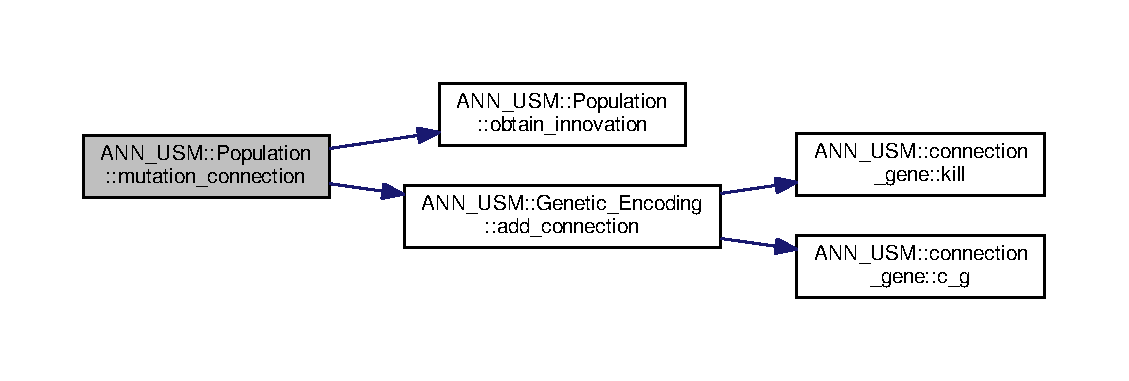
\includegraphics[width=350pt]{class_a_n_n___u_s_m_1_1_population_acee4c5ba8e56deb1386864d349d78316_cgraph}
\end{center}
\end{figure}




Here is the caller graph for this function\-:\nopagebreak
\begin{figure}[H]
\begin{center}
\leavevmode
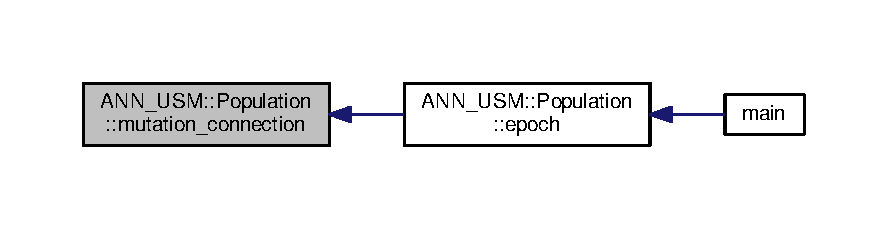
\includegraphics[width=350pt]{class_a_n_n___u_s_m_1_1_population_acee4c5ba8e56deb1386864d349d78316_icgraph}
\end{center}
\end{figure}


\hypertarget{class_a_n_n___u_s_m_1_1_population_a20ca394c0565450c1843333129057027}{\index{A\-N\-N\-\_\-\-U\-S\-M\-::\-Population@{A\-N\-N\-\_\-\-U\-S\-M\-::\-Population}!mutation\-\_\-node@{mutation\-\_\-node}}
\index{mutation\-\_\-node@{mutation\-\_\-node}!ANN_USM::Population@{A\-N\-N\-\_\-\-U\-S\-M\-::\-Population}}
\subsubsection[{mutation\-\_\-node}]{\setlength{\rightskip}{0pt plus 5cm}{\bf Genetic\-\_\-\-Encoding} Population\-::mutation\-\_\-node (
\begin{DoxyParamCaption}
\item[{{\bf Genetic\-\_\-\-Encoding}}]{organism}
\end{DoxyParamCaption}
)}}\label{class_a_n_n___u_s_m_1_1_population_a20ca394c0565450c1843333129057027}


Definition at line 68 of file C\-P\-P\-N-\/\-N\-E\-A\-T.\-cpp.



Here is the call graph for this function\-:\nopagebreak
\begin{figure}[H]
\begin{center}
\leavevmode
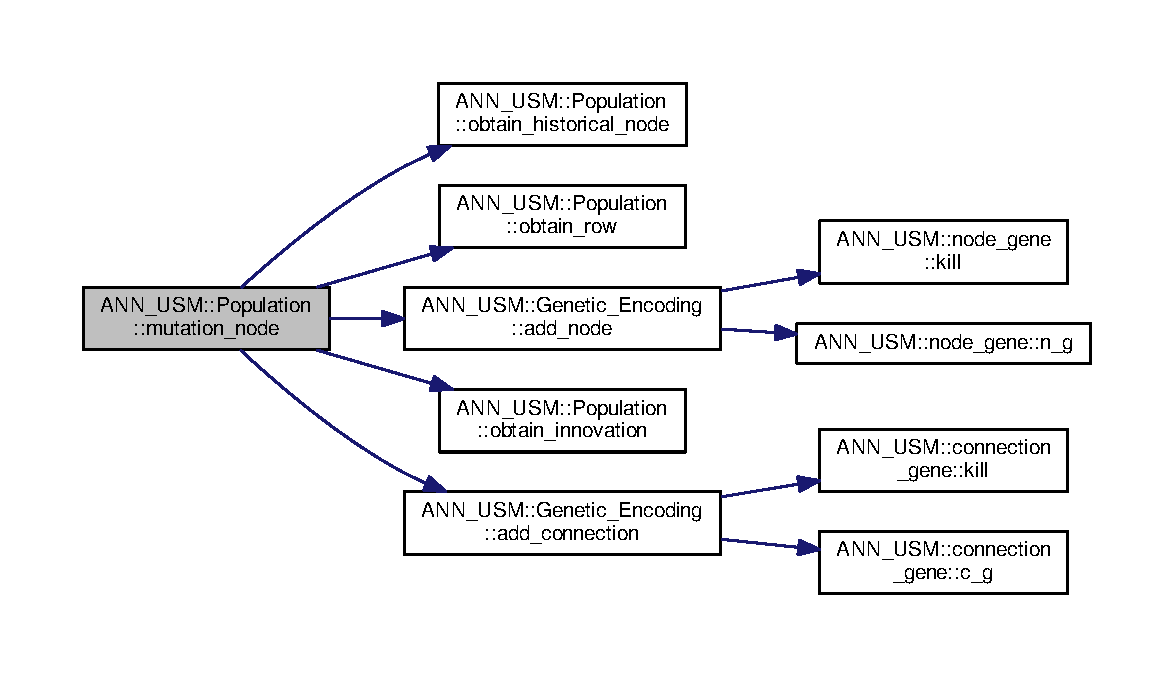
\includegraphics[width=350pt]{class_a_n_n___u_s_m_1_1_population_a20ca394c0565450c1843333129057027_cgraph}
\end{center}
\end{figure}




Here is the caller graph for this function\-:\nopagebreak
\begin{figure}[H]
\begin{center}
\leavevmode
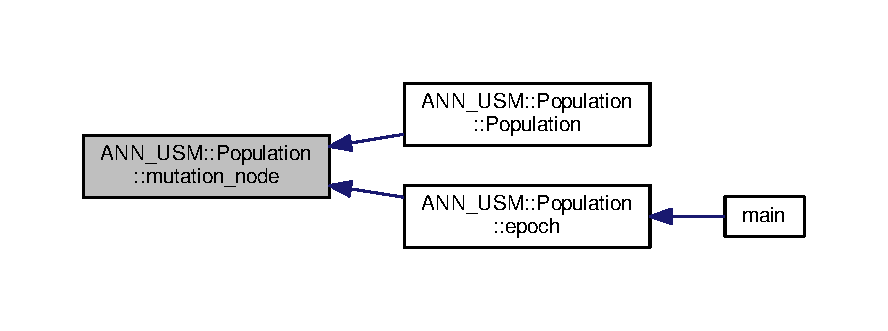
\includegraphics[width=350pt]{class_a_n_n___u_s_m_1_1_population_a20ca394c0565450c1843333129057027_icgraph}
\end{center}
\end{figure}


\hypertarget{class_a_n_n___u_s_m_1_1_population_a037c144dd6c90391d312a1b38af6e057}{\index{A\-N\-N\-\_\-\-U\-S\-M\-::\-Population@{A\-N\-N\-\_\-\-U\-S\-M\-::\-Population}!obtain\-\_\-historical\-\_\-node@{obtain\-\_\-historical\-\_\-node}}
\index{obtain\-\_\-historical\-\_\-node@{obtain\-\_\-historical\-\_\-node}!ANN_USM::Population@{A\-N\-N\-\_\-\-U\-S\-M\-::\-Population}}
\subsubsection[{obtain\-\_\-historical\-\_\-node}]{\setlength{\rightskip}{0pt plus 5cm}int Population\-::obtain\-\_\-historical\-\_\-node (
\begin{DoxyParamCaption}
\item[{int}]{initial\-\_\-in, }
\item[{int}]{initial\-\_\-out}
\end{DoxyParamCaption}
)}}\label{class_a_n_n___u_s_m_1_1_population_a037c144dd6c90391d312a1b38af6e057}


Definition at line 193 of file C\-P\-P\-N-\/\-N\-E\-A\-T.\-cpp.



Here is the caller graph for this function\-:\nopagebreak
\begin{figure}[H]
\begin{center}
\leavevmode
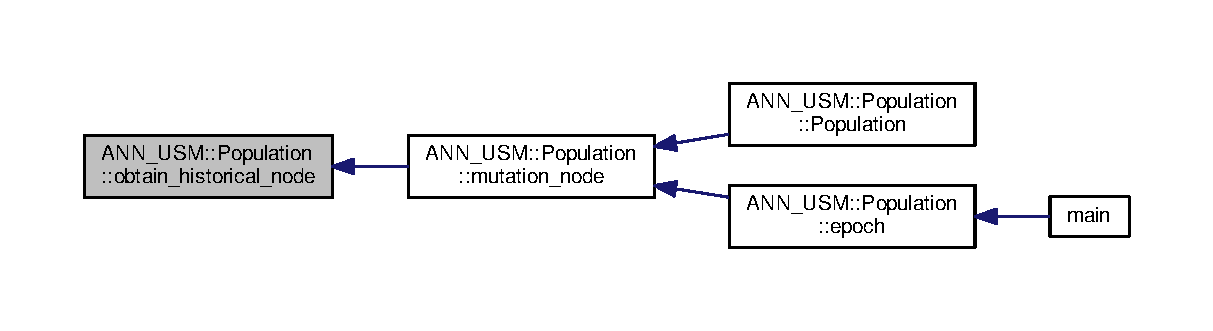
\includegraphics[width=350pt]{class_a_n_n___u_s_m_1_1_population_a037c144dd6c90391d312a1b38af6e057_icgraph}
\end{center}
\end{figure}


\hypertarget{class_a_n_n___u_s_m_1_1_population_a16090fdb0f1e89cc91568028777ac847}{\index{A\-N\-N\-\_\-\-U\-S\-M\-::\-Population@{A\-N\-N\-\_\-\-U\-S\-M\-::\-Population}!obtain\-\_\-innovation@{obtain\-\_\-innovation}}
\index{obtain\-\_\-innovation@{obtain\-\_\-innovation}!ANN_USM::Population@{A\-N\-N\-\_\-\-U\-S\-M\-::\-Population}}
\subsubsection[{obtain\-\_\-innovation}]{\setlength{\rightskip}{0pt plus 5cm}int Population\-::obtain\-\_\-innovation (
\begin{DoxyParamCaption}
\item[{int}]{in, }
\item[{int}]{out}
\end{DoxyParamCaption}
)}}\label{class_a_n_n___u_s_m_1_1_population_a16090fdb0f1e89cc91568028777ac847}


Obtain the (historical) innovation number between two nodes. 

If both nodes were connected at any time in the past then they will have the very same innovation number they had earlier.

If they weren't connected at all then they will have a new innovation number, filling every vector in between with -\/1, i.\-e. not connected. If the inner node of the connection is greater than the vector size, fill with empty vectors until reach the desired node.

If the outgoing node of the connection is greater than the vector size at the inner position, fill with -\/1 until reach the desired node.

If the desired pair of nodes was not connected in the past, give the new innovation number to the connection and increase in one the innovation number.

If it was connected then skip the if statement and return the innovation number of the pair of nodes.

Definition at line 215 of file C\-P\-P\-N-\/\-N\-E\-A\-T.\-cpp.



Here is the caller graph for this function\-:\nopagebreak
\begin{figure}[H]
\begin{center}
\leavevmode
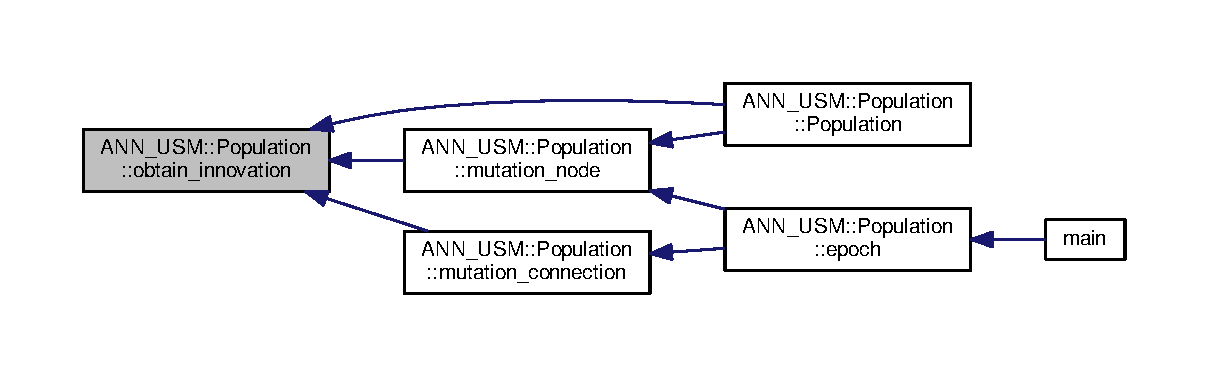
\includegraphics[width=350pt]{class_a_n_n___u_s_m_1_1_population_a16090fdb0f1e89cc91568028777ac847_icgraph}
\end{center}
\end{figure}


\hypertarget{class_a_n_n___u_s_m_1_1_population_a84ab90f06fe08ed2b95638427086a331}{\index{A\-N\-N\-\_\-\-U\-S\-M\-::\-Population@{A\-N\-N\-\_\-\-U\-S\-M\-::\-Population}!obtain\-\_\-row@{obtain\-\_\-row}}
\index{obtain\-\_\-row@{obtain\-\_\-row}!ANN_USM::Population@{A\-N\-N\-\_\-\-U\-S\-M\-::\-Population}}
\subsubsection[{obtain\-\_\-row}]{\setlength{\rightskip}{0pt plus 5cm}int Population\-::obtain\-\_\-row (
\begin{DoxyParamCaption}
\item[{int}]{node, }
\item[{int}]{node\-\_\-initial\-\_\-in, }
\item[{int}]{node\-\_\-initial\-\_\-out}
\end{DoxyParamCaption}
)}}\label{class_a_n_n___u_s_m_1_1_population_a84ab90f06fe08ed2b95638427086a331}


Definition at line 126 of file C\-P\-P\-N-\/\-N\-E\-A\-T.\-cpp.



Here is the caller graph for this function\-:\nopagebreak
\begin{figure}[H]
\begin{center}
\leavevmode
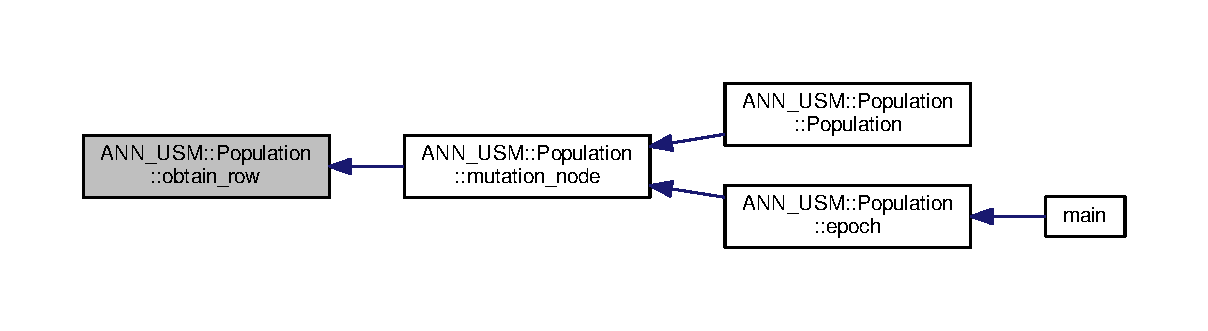
\includegraphics[width=350pt]{class_a_n_n___u_s_m_1_1_population_a84ab90f06fe08ed2b95638427086a331_icgraph}
\end{center}
\end{figure}


\hypertarget{class_a_n_n___u_s_m_1_1_population_a0b858ba5af6628979fd7f136520cdd5b}{\index{A\-N\-N\-\_\-\-U\-S\-M\-::\-Population@{A\-N\-N\-\_\-\-U\-S\-M\-::\-Population}!put\-\_\-randoms\-\_\-weight@{put\-\_\-randoms\-\_\-weight}}
\index{put\-\_\-randoms\-\_\-weight@{put\-\_\-randoms\-\_\-weight}!ANN_USM::Population@{A\-N\-N\-\_\-\-U\-S\-M\-::\-Population}}
\subsubsection[{put\-\_\-randoms\-\_\-weight}]{\setlength{\rightskip}{0pt plus 5cm}{\bf Genetic\-\_\-\-Encoding} Population\-::put\-\_\-randoms\-\_\-weight (
\begin{DoxyParamCaption}
\item[{{\bf Genetic\-\_\-\-Encoding}}]{organism}
\end{DoxyParamCaption}
)}}\label{class_a_n_n___u_s_m_1_1_population_a0b858ba5af6628979fd7f136520cdd5b}


Definition at line 49 of file C\-P\-P\-N-\/\-N\-E\-A\-T.\-cpp.



Here is the caller graph for this function\-:\nopagebreak
\begin{figure}[H]
\begin{center}
\leavevmode
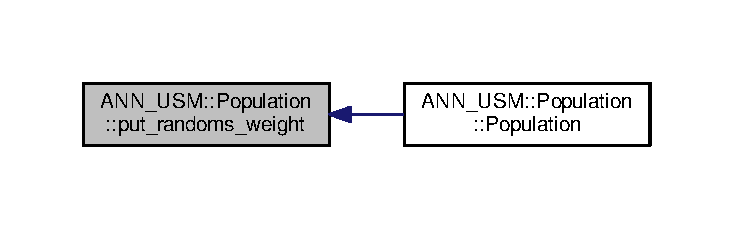
\includegraphics[width=350pt]{class_a_n_n___u_s_m_1_1_population_a0b858ba5af6628979fd7f136520cdd5b_icgraph}
\end{center}
\end{figure}


\hypertarget{class_a_n_n___u_s_m_1_1_population_ad6a8d08fc4f4cbcc84405ddd7e40a453}{\index{A\-N\-N\-\_\-\-U\-S\-M\-::\-Population@{A\-N\-N\-\_\-\-U\-S\-M\-::\-Population}!save@{save}}
\index{save@{save}!ANN_USM::Population@{A\-N\-N\-\_\-\-U\-S\-M\-::\-Population}}
\subsubsection[{save}]{\setlength{\rightskip}{0pt plus 5cm}void Population\-::save (
\begin{DoxyParamCaption}
\item[{char}]{path\mbox{[}$\,$\mbox{]}}
\end{DoxyParamCaption}
)}}\label{class_a_n_n___u_s_m_1_1_population_ad6a8d08fc4f4cbcc84405ddd7e40a453}


Definition at line 334 of file C\-P\-P\-N-\/\-N\-E\-A\-T.\-cpp.



Here is the call graph for this function\-:\nopagebreak
\begin{figure}[H]
\begin{center}
\leavevmode
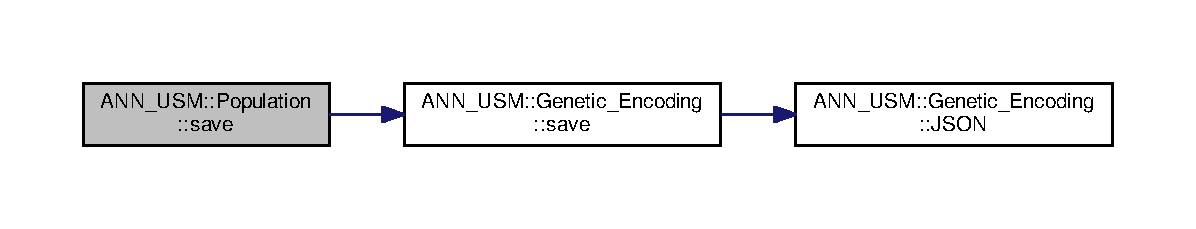
\includegraphics[width=350pt]{class_a_n_n___u_s_m_1_1_population_ad6a8d08fc4f4cbcc84405ddd7e40a453_cgraph}
\end{center}
\end{figure}




Here is the caller graph for this function\-:\nopagebreak
\begin{figure}[H]
\begin{center}
\leavevmode
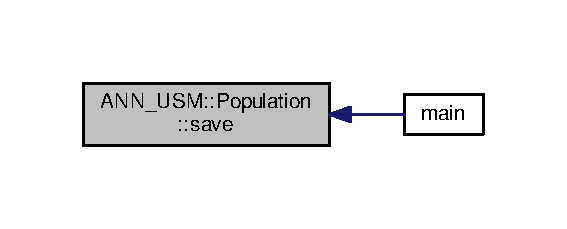
\includegraphics[width=272pt]{class_a_n_n___u_s_m_1_1_population_ad6a8d08fc4f4cbcc84405ddd7e40a453_icgraph}
\end{center}
\end{figure}


\hypertarget{class_a_n_n___u_s_m_1_1_population_af15b09e6b9ca34cf5c7f15fe33d1c5bb}{\index{A\-N\-N\-\_\-\-U\-S\-M\-::\-Population@{A\-N\-N\-\_\-\-U\-S\-M\-::\-Population}!save\-\_\-all@{save\-\_\-all}}
\index{save\-\_\-all@{save\-\_\-all}!ANN_USM::Population@{A\-N\-N\-\_\-\-U\-S\-M\-::\-Population}}
\subsubsection[{save\-\_\-all}]{\setlength{\rightskip}{0pt plus 5cm}void Population\-::save\-\_\-all (
\begin{DoxyParamCaption}
\item[{char}]{path\mbox{[}$\,$\mbox{]}}
\end{DoxyParamCaption}
)}}\label{class_a_n_n___u_s_m_1_1_population_af15b09e6b9ca34cf5c7f15fe33d1c5bb}


Definition at line 326 of file C\-P\-P\-N-\/\-N\-E\-A\-T.\-cpp.

\hypertarget{class_a_n_n___u_s_m_1_1_population_aa14d8cb45306aa8b9851791a6d547be6}{\index{A\-N\-N\-\_\-\-U\-S\-M\-::\-Population@{A\-N\-N\-\_\-\-U\-S\-M\-::\-Population}!spatiation@{spatiation}}
\index{spatiation@{spatiation}!ANN_USM::Population@{A\-N\-N\-\_\-\-U\-S\-M\-::\-Population}}
\subsubsection[{spatiation}]{\setlength{\rightskip}{0pt plus 5cm}void Population\-::spatiation (
\begin{DoxyParamCaption}
{}
\end{DoxyParamCaption}
)}}\label{class_a_n_n___u_s_m_1_1_population_aa14d8cb45306aa8b9851791a6d547be6}


Definition at line 469 of file C\-P\-P\-N-\/\-N\-E\-A\-T.\-cpp.



Here is the call graph for this function\-:\nopagebreak
\begin{figure}[H]
\begin{center}
\leavevmode
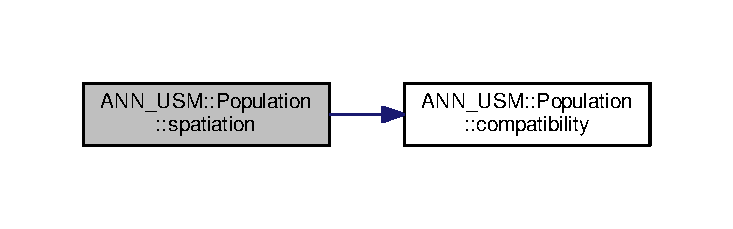
\includegraphics[width=350pt]{class_a_n_n___u_s_m_1_1_population_aa14d8cb45306aa8b9851791a6d547be6_cgraph}
\end{center}
\end{figure}




Here is the caller graph for this function\-:\nopagebreak
\begin{figure}[H]
\begin{center}
\leavevmode
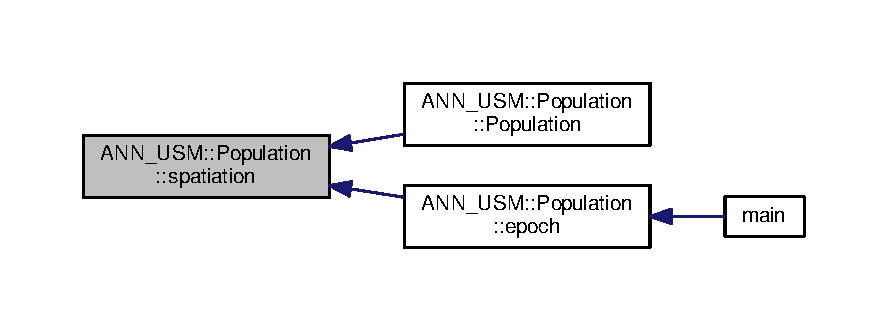
\includegraphics[width=350pt]{class_a_n_n___u_s_m_1_1_population_aa14d8cb45306aa8b9851791a6d547be6_icgraph}
\end{center}
\end{figure}




\subsection{Member Data Documentation}
\hypertarget{class_a_n_n___u_s_m_1_1_population_a00cc470bf44ddbb9c104d3eead923dc3}{\index{A\-N\-N\-\_\-\-U\-S\-M\-::\-Population@{A\-N\-N\-\_\-\-U\-S\-M\-::\-Population}!best\-\_\-organism@{best\-\_\-organism}}
\index{best\-\_\-organism@{best\-\_\-organism}!ANN_USM::Population@{A\-N\-N\-\_\-\-U\-S\-M\-::\-Population}}
\subsubsection[{best\-\_\-organism}]{\setlength{\rightskip}{0pt plus 5cm}{\bf Genetic\-\_\-\-Encoding}$\ast$ A\-N\-N\-\_\-\-U\-S\-M\-::\-Population\-::best\-\_\-organism}}\label{class_a_n_n___u_s_m_1_1_population_a00cc470bf44ddbb9c104d3eead923dc3}


Definition at line 75 of file C\-P\-P\-N-\/\-N\-E\-A\-T.\-hpp.

\hypertarget{class_a_n_n___u_s_m_1_1_population_a8fadd74c69061f51a5e3ea9a3d4aa516}{\index{A\-N\-N\-\_\-\-U\-S\-M\-::\-Population@{A\-N\-N\-\_\-\-U\-S\-M\-::\-Population}!champion@{champion}}
\index{champion@{champion}!ANN_USM::Population@{A\-N\-N\-\_\-\-U\-S\-M\-::\-Population}}
\subsubsection[{champion}]{\setlength{\rightskip}{0pt plus 5cm}{\bf Genetic\-\_\-\-Encoding} A\-N\-N\-\_\-\-U\-S\-M\-::\-Population\-::champion}}\label{class_a_n_n___u_s_m_1_1_population_a8fadd74c69061f51a5e3ea9a3d4aa516}


Definition at line 76 of file C\-P\-P\-N-\/\-N\-E\-A\-T.\-hpp.

\hypertarget{class_a_n_n___u_s_m_1_1_population_aa45357359720f5ce88603d0282d22f17}{\index{A\-N\-N\-\_\-\-U\-S\-M\-::\-Population@{A\-N\-N\-\_\-\-U\-S\-M\-::\-Population}!current\-\_\-niches@{current\-\_\-niches}}
\index{current\-\_\-niches@{current\-\_\-niches}!ANN_USM::Population@{A\-N\-N\-\_\-\-U\-S\-M\-::\-Population}}
\subsubsection[{current\-\_\-niches}]{\setlength{\rightskip}{0pt plus 5cm}vector$<${\bf Niche}$>$ A\-N\-N\-\_\-\-U\-S\-M\-::\-Population\-::current\-\_\-niches}}\label{class_a_n_n___u_s_m_1_1_population_aa45357359720f5ce88603d0282d22f17}


Definition at line 72 of file C\-P\-P\-N-\/\-N\-E\-A\-T.\-hpp.

\hypertarget{class_a_n_n___u_s_m_1_1_population_a0622623a426583853cd7cc1e16bd9423}{\index{A\-N\-N\-\_\-\-U\-S\-M\-::\-Population@{A\-N\-N\-\_\-\-U\-S\-M\-::\-Population}!fitness\-\_\-champion@{fitness\-\_\-champion}}
\index{fitness\-\_\-champion@{fitness\-\_\-champion}!ANN_USM::Population@{A\-N\-N\-\_\-\-U\-S\-M\-::\-Population}}
\subsubsection[{fitness\-\_\-champion}]{\setlength{\rightskip}{0pt plus 5cm}double A\-N\-N\-\_\-\-U\-S\-M\-::\-Population\-::fitness\-\_\-champion}}\label{class_a_n_n___u_s_m_1_1_population_a0622623a426583853cd7cc1e16bd9423}


Definition at line 67 of file C\-P\-P\-N-\/\-N\-E\-A\-T.\-hpp.

\hypertarget{class_a_n_n___u_s_m_1_1_population_a980dc824cafc3dd2750f87c3300cdb95}{\index{A\-N\-N\-\_\-\-U\-S\-M\-::\-Population@{A\-N\-N\-\_\-\-U\-S\-M\-::\-Population}!historical\-\_\-innovation@{historical\-\_\-innovation}}
\index{historical\-\_\-innovation@{historical\-\_\-innovation}!ANN_USM::Population@{A\-N\-N\-\_\-\-U\-S\-M\-::\-Population}}
\subsubsection[{historical\-\_\-innovation}]{\setlength{\rightskip}{0pt plus 5cm}vector$<$ vector$<$int$>$ $>$ A\-N\-N\-\_\-\-U\-S\-M\-::\-Population\-::historical\-\_\-innovation}}\label{class_a_n_n___u_s_m_1_1_population_a980dc824cafc3dd2750f87c3300cdb95}


Definition at line 79 of file C\-P\-P\-N-\/\-N\-E\-A\-T.\-hpp.

\hypertarget{class_a_n_n___u_s_m_1_1_population_a5cbc92463b8bf0cc1031441ecfcd16bf}{\index{A\-N\-N\-\_\-\-U\-S\-M\-::\-Population@{A\-N\-N\-\_\-\-U\-S\-M\-::\-Population}!historical\-\_\-nodes@{historical\-\_\-nodes}}
\index{historical\-\_\-nodes@{historical\-\_\-nodes}!ANN_USM::Population@{A\-N\-N\-\_\-\-U\-S\-M\-::\-Population}}
\subsubsection[{historical\-\_\-nodes}]{\setlength{\rightskip}{0pt plus 5cm}vector$<$ vector$<$int$>$ $>$ A\-N\-N\-\_\-\-U\-S\-M\-::\-Population\-::historical\-\_\-nodes}}\label{class_a_n_n___u_s_m_1_1_population_a5cbc92463b8bf0cc1031441ecfcd16bf}


Definition at line 78 of file C\-P\-P\-N-\/\-N\-E\-A\-T.\-hpp.

\hypertarget{class_a_n_n___u_s_m_1_1_population_ad2643c1369c231da3de9878dfaa0ccf2}{\index{A\-N\-N\-\_\-\-U\-S\-M\-::\-Population@{A\-N\-N\-\_\-\-U\-S\-M\-::\-Population}!historical\-\_\-row@{historical\-\_\-row}}
\index{historical\-\_\-row@{historical\-\_\-row}!ANN_USM::Population@{A\-N\-N\-\_\-\-U\-S\-M\-::\-Population}}
\subsubsection[{historical\-\_\-row}]{\setlength{\rightskip}{0pt plus 5cm}vector$<$int$>$ A\-N\-N\-\_\-\-U\-S\-M\-::\-Population\-::historical\-\_\-row}}\label{class_a_n_n___u_s_m_1_1_population_ad2643c1369c231da3de9878dfaa0ccf2}


Definition at line 81 of file C\-P\-P\-N-\/\-N\-E\-A\-T.\-hpp.

\hypertarget{class_a_n_n___u_s_m_1_1_population_a836ae3c612ff56cac400ddea08893961}{\index{A\-N\-N\-\_\-\-U\-S\-M\-::\-Population@{A\-N\-N\-\_\-\-U\-S\-M\-::\-Population}!last\-\_\-innovation@{last\-\_\-innovation}}
\index{last\-\_\-innovation@{last\-\_\-innovation}!ANN_USM::Population@{A\-N\-N\-\_\-\-U\-S\-M\-::\-Population}}
\subsubsection[{last\-\_\-innovation}]{\setlength{\rightskip}{0pt plus 5cm}int A\-N\-N\-\_\-\-U\-S\-M\-::\-Population\-::last\-\_\-innovation}}\label{class_a_n_n___u_s_m_1_1_population_a836ae3c612ff56cac400ddea08893961}


Definition at line 63 of file C\-P\-P\-N-\/\-N\-E\-A\-T.\-hpp.

\hypertarget{class_a_n_n___u_s_m_1_1_population_a609df33a9f9f1221ddf5604ef01dace5}{\index{A\-N\-N\-\_\-\-U\-S\-M\-::\-Population@{A\-N\-N\-\_\-\-U\-S\-M\-::\-Population}!last\-\_\-niche\-\_\-id@{last\-\_\-niche\-\_\-id}}
\index{last\-\_\-niche\-\_\-id@{last\-\_\-niche\-\_\-id}!ANN_USM::Population@{A\-N\-N\-\_\-\-U\-S\-M\-::\-Population}}
\subsubsection[{last\-\_\-niche\-\_\-id}]{\setlength{\rightskip}{0pt plus 5cm}int A\-N\-N\-\_\-\-U\-S\-M\-::\-Population\-::last\-\_\-niche\-\_\-id}}\label{class_a_n_n___u_s_m_1_1_population_a609df33a9f9f1221ddf5604ef01dace5}


Definition at line 62 of file C\-P\-P\-N-\/\-N\-E\-A\-T.\-hpp.

\hypertarget{class_a_n_n___u_s_m_1_1_population_a2c53f59115f21a4b42e91f8aca35cdcf}{\index{A\-N\-N\-\_\-\-U\-S\-M\-::\-Population@{A\-N\-N\-\_\-\-U\-S\-M\-::\-Population}!last\-\_\-node@{last\-\_\-node}}
\index{last\-\_\-node@{last\-\_\-node}!ANN_USM::Population@{A\-N\-N\-\_\-\-U\-S\-M\-::\-Population}}
\subsubsection[{last\-\_\-node}]{\setlength{\rightskip}{0pt plus 5cm}int A\-N\-N\-\_\-\-U\-S\-M\-::\-Population\-::last\-\_\-node}}\label{class_a_n_n___u_s_m_1_1_population_a2c53f59115f21a4b42e91f8aca35cdcf}


Definition at line 64 of file C\-P\-P\-N-\/\-N\-E\-A\-T.\-hpp.

\hypertarget{class_a_n_n___u_s_m_1_1_population_a158d58cd6154506562b3a4b4cc563034}{\index{A\-N\-N\-\_\-\-U\-S\-M\-::\-Population@{A\-N\-N\-\_\-\-U\-S\-M\-::\-Population}!last\-\_\-row@{last\-\_\-row}}
\index{last\-\_\-row@{last\-\_\-row}!ANN_USM::Population@{A\-N\-N\-\_\-\-U\-S\-M\-::\-Population}}
\subsubsection[{last\-\_\-row}]{\setlength{\rightskip}{0pt plus 5cm}int A\-N\-N\-\_\-\-U\-S\-M\-::\-Population\-::last\-\_\-row}}\label{class_a_n_n___u_s_m_1_1_population_a158d58cd6154506562b3a4b4cc563034}


Definition at line 65 of file C\-P\-P\-N-\/\-N\-E\-A\-T.\-hpp.

\hypertarget{class_a_n_n___u_s_m_1_1_population_a9a9980d69d2a013d4dfc1388b7d96db6}{\index{A\-N\-N\-\_\-\-U\-S\-M\-::\-Population@{A\-N\-N\-\_\-\-U\-S\-M\-::\-Population}!lenght@{lenght}}
\index{lenght@{lenght}!ANN_USM::Population@{A\-N\-N\-\_\-\-U\-S\-M\-::\-Population}}
\subsubsection[{lenght}]{\setlength{\rightskip}{0pt plus 5cm}int A\-N\-N\-\_\-\-U\-S\-M\-::\-Population\-::lenght}}\label{class_a_n_n___u_s_m_1_1_population_a9a9980d69d2a013d4dfc1388b7d96db6}


Definition at line 60 of file C\-P\-P\-N-\/\-N\-E\-A\-T.\-hpp.

\hypertarget{class_a_n_n___u_s_m_1_1_population_a98468ee8221857cad41ae4d7b2ae01cf}{\index{A\-N\-N\-\_\-\-U\-S\-M\-::\-Population@{A\-N\-N\-\_\-\-U\-S\-M\-::\-Population}!organisms@{organisms}}
\index{organisms@{organisms}!ANN_USM::Population@{A\-N\-N\-\_\-\-U\-S\-M\-::\-Population}}
\subsubsection[{organisms}]{\setlength{\rightskip}{0pt plus 5cm}vector$<${\bf Genetic\-\_\-\-Encoding}$>$ A\-N\-N\-\_\-\-U\-S\-M\-::\-Population\-::organisms}}\label{class_a_n_n___u_s_m_1_1_population_a98468ee8221857cad41ae4d7b2ae01cf}


Definition at line 69 of file C\-P\-P\-N-\/\-N\-E\-A\-T.\-hpp.

\hypertarget{class_a_n_n___u_s_m_1_1_population_a1103c56991771d6ccae5e1cccaf51db9}{\index{A\-N\-N\-\_\-\-U\-S\-M\-::\-Population@{A\-N\-N\-\_\-\-U\-S\-M\-::\-Population}!prev\-\_\-niches@{prev\-\_\-niches}}
\index{prev\-\_\-niches@{prev\-\_\-niches}!ANN_USM::Population@{A\-N\-N\-\_\-\-U\-S\-M\-::\-Population}}
\subsubsection[{prev\-\_\-niches}]{\setlength{\rightskip}{0pt plus 5cm}vector$<${\bf Niche}$>$ A\-N\-N\-\_\-\-U\-S\-M\-::\-Population\-::prev\-\_\-niches}}\label{class_a_n_n___u_s_m_1_1_population_a1103c56991771d6ccae5e1cccaf51db9}


Definition at line 73 of file C\-P\-P\-N-\/\-N\-E\-A\-T.\-hpp.

\hypertarget{class_a_n_n___u_s_m_1_1_population_ad1ba3ace7157e2763976a1ee1155584b}{\index{A\-N\-N\-\_\-\-U\-S\-M\-::\-Population@{A\-N\-N\-\_\-\-U\-S\-M\-::\-Population}!prev\-\_\-organisms@{prev\-\_\-organisms}}
\index{prev\-\_\-organisms@{prev\-\_\-organisms}!ANN_USM::Population@{A\-N\-N\-\_\-\-U\-S\-M\-::\-Population}}
\subsubsection[{prev\-\_\-organisms}]{\setlength{\rightskip}{0pt plus 5cm}vector$<${\bf Genetic\-\_\-\-Encoding}$>$ A\-N\-N\-\_\-\-U\-S\-M\-::\-Population\-::prev\-\_\-organisms}}\label{class_a_n_n___u_s_m_1_1_population_ad1ba3ace7157e2763976a1ee1155584b}


Definition at line 70 of file C\-P\-P\-N-\/\-N\-E\-A\-T.\-hpp.

\hypertarget{class_a_n_n___u_s_m_1_1_population_ae688b66299b4b8be34d34a797bbc44ab}{\index{A\-N\-N\-\_\-\-U\-S\-M\-::\-Population@{A\-N\-N\-\_\-\-U\-S\-M\-::\-Population}!row\-\_\-orderer\-\_\-list@{row\-\_\-orderer\-\_\-list}}
\index{row\-\_\-orderer\-\_\-list@{row\-\_\-orderer\-\_\-list}!ANN_USM::Population@{A\-N\-N\-\_\-\-U\-S\-M\-::\-Population}}
\subsubsection[{row\-\_\-orderer\-\_\-list}]{\setlength{\rightskip}{0pt plus 5cm}vector$<$int$>$ A\-N\-N\-\_\-\-U\-S\-M\-::\-Population\-::row\-\_\-orderer\-\_\-list}}\label{class_a_n_n___u_s_m_1_1_population_ae688b66299b4b8be34d34a797bbc44ab}


Definition at line 82 of file C\-P\-P\-N-\/\-N\-E\-A\-T.\-hpp.

\hypertarget{class_a_n_n___u_s_m_1_1_population_a5dd00b369c21214466d0f155ba0e11ee}{\index{A\-N\-N\-\_\-\-U\-S\-M\-::\-Population@{A\-N\-N\-\_\-\-U\-S\-M\-::\-Population}!total\-\_\-niches@{total\-\_\-niches}}
\index{total\-\_\-niches@{total\-\_\-niches}!ANN_USM::Population@{A\-N\-N\-\_\-\-U\-S\-M\-::\-Population}}
\subsubsection[{total\-\_\-niches}]{\setlength{\rightskip}{0pt plus 5cm}int A\-N\-N\-\_\-\-U\-S\-M\-::\-Population\-::total\-\_\-niches}}\label{class_a_n_n___u_s_m_1_1_population_a5dd00b369c21214466d0f155ba0e11ee}


Definition at line 61 of file C\-P\-P\-N-\/\-N\-E\-A\-T.\-hpp.



The documentation for this class was generated from the following files\-:\begin{DoxyCompactItemize}
\item 
headers/\hyperlink{_c_p_p_n-_n_e_a_t_8hpp}{C\-P\-P\-N-\/\-N\-E\-A\-T.\-hpp}\item 
src/\hyperlink{_c_p_p_n-_n_e_a_t_8cpp}{C\-P\-P\-N-\/\-N\-E\-A\-T.\-cpp}\end{DoxyCompactItemize}

\chapter{File Documentation}
\hypertarget{_c_p_p_n-_n_e_a_t_8hpp}{\section{headers/\-C\-P\-P\-N-\/\-N\-E\-A\-T.hpp File Reference}
\label{_c_p_p_n-_n_e_a_t_8hpp}\index{headers/\-C\-P\-P\-N-\/\-N\-E\-A\-T.\-hpp@{headers/\-C\-P\-P\-N-\/\-N\-E\-A\-T.\-hpp}}
}
{\ttfamily \#include $<$cmath$>$}\\*
{\ttfamily \#include $<$unistd.\-h$>$}\\*
{\ttfamily \#include \char`\"{}fitness.\-hpp\char`\"{}}\\*
{\ttfamily \#include \char`\"{}genetic\-\_\-encoding.\-hpp\char`\"{}}\\*
{\ttfamily \#include \char`\"{}user\-\_\-definitions.\-hpp\char`\"{}}\\*
Include dependency graph for C\-P\-P\-N-\/\-N\-E\-A\-T.hpp\-:
\nopagebreak
\begin{figure}[H]
\begin{center}
\leavevmode
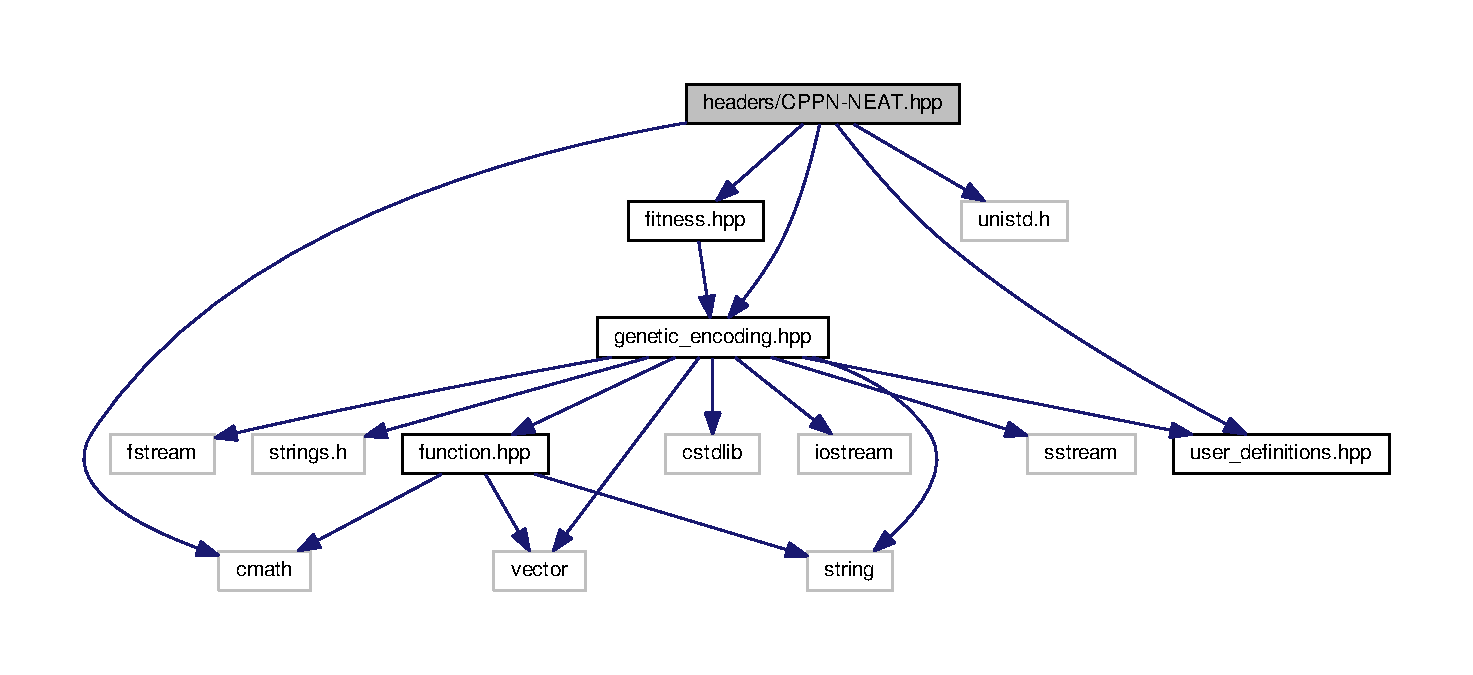
\includegraphics[width=350pt]{_c_p_p_n-_n_e_a_t_8hpp__incl}
\end{center}
\end{figure}
This graph shows which files directly or indirectly include this file\-:
\nopagebreak
\begin{figure}[H]
\begin{center}
\leavevmode
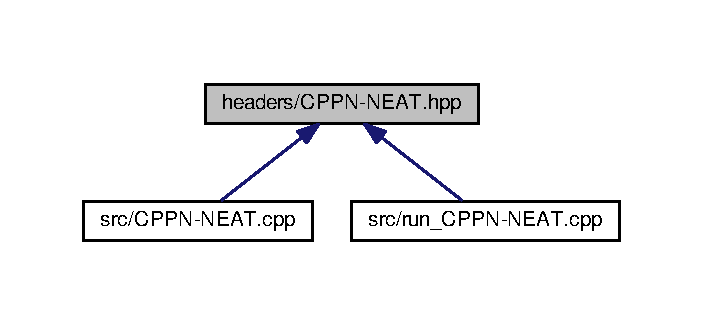
\includegraphics[width=337pt]{_c_p_p_n-_n_e_a_t_8hpp__dep__incl}
\end{center}
\end{figure}
\subsection*{Classes}
\begin{DoxyCompactItemize}
\item 
class \hyperlink{class_a_n_n___u_s_m_1_1_niche}{A\-N\-N\-\_\-\-U\-S\-M\-::\-Niche}
\item 
class \hyperlink{class_a_n_n___u_s_m_1_1_population}{A\-N\-N\-\_\-\-U\-S\-M\-::\-Population}
\end{DoxyCompactItemize}
\subsection*{Namespaces}
\begin{DoxyCompactItemize}
\item 
\hyperlink{namespace_a_n_n___u_s_m}{A\-N\-N\-\_\-\-U\-S\-M}
\end{DoxyCompactItemize}
\subsection*{Functions}
\begin{DoxyCompactItemize}
\item 
ostream \& \hyperlink{_c_p_p_n-_n_e_a_t_8hpp_a81655a8d2a9e6437481493618f945ea4}{operator$<$$<$} (ostream \&o, \hyperlink{class_a_n_n___u_s_m_1_1_population}{A\-N\-N\-\_\-\-U\-S\-M\-::\-Population} \&pop)
\end{DoxyCompactItemize}


\subsection{Function Documentation}
\hypertarget{_c_p_p_n-_n_e_a_t_8hpp_a81655a8d2a9e6437481493618f945ea4}{\index{C\-P\-P\-N-\/\-N\-E\-A\-T.\-hpp@{C\-P\-P\-N-\/\-N\-E\-A\-T.\-hpp}!operator$<$$<$@{operator$<$$<$}}
\index{operator$<$$<$@{operator$<$$<$}!CPPN-NEAT.hpp@{C\-P\-P\-N-\/\-N\-E\-A\-T.\-hpp}}
\subsubsection[{operator$<$$<$}]{\setlength{\rightskip}{0pt plus 5cm}ostream\& operator$<$$<$ (
\begin{DoxyParamCaption}
\item[{ostream \&}]{o, }
\item[{{\bf A\-N\-N\-\_\-\-U\-S\-M\-::\-Population} \&}]{pop}
\end{DoxyParamCaption}
)}}\label{_c_p_p_n-_n_e_a_t_8hpp_a81655a8d2a9e6437481493618f945ea4}


Definition at line 315 of file C\-P\-P\-N-\/\-N\-E\-A\-T.\-cpp.


\hypertarget{fitness_8hpp}{\section{headers/fitness.hpp File Reference}
\label{fitness_8hpp}\index{headers/fitness.\-hpp@{headers/fitness.\-hpp}}
}
{\ttfamily \#include \char`\"{}genetic\-\_\-encoding.\-hpp\char`\"{}}\\*
Include dependency graph for fitness.\-hpp\-:
\nopagebreak
\begin{figure}[H]
\begin{center}
\leavevmode
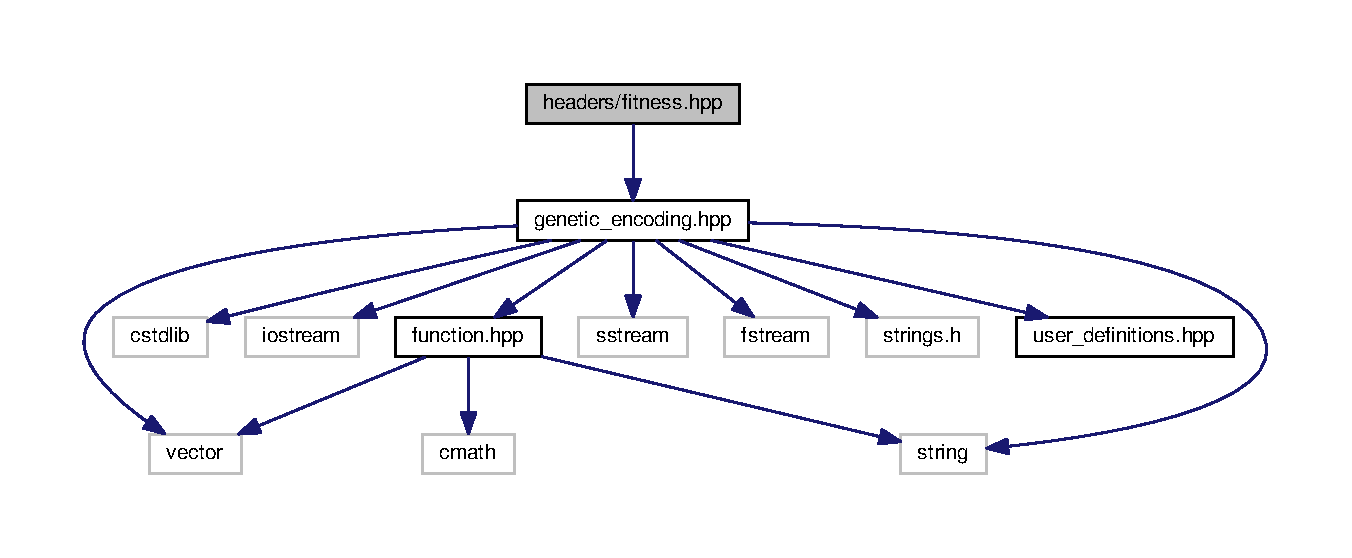
\includegraphics[width=350pt]{fitness_8hpp__incl}
\end{center}
\end{figure}
This graph shows which files directly or indirectly include this file\-:
\nopagebreak
\begin{figure}[H]
\begin{center}
\leavevmode
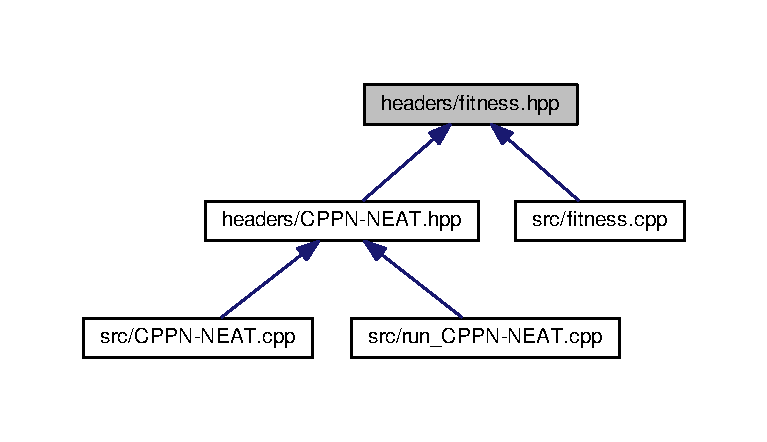
\includegraphics[width=350pt]{fitness_8hpp__dep__incl}
\end{center}
\end{figure}
\subsection*{Functions}
\begin{DoxyCompactItemize}
\item 
double \hyperlink{fitness_8hpp_ab547101b5cc5b5c2957842bea97514ce}{fitness} (\hyperlink{class_a_n_n___u_s_m_1_1_genetic___encoding}{Genetic\-\_\-\-Encoding} organism)
\end{DoxyCompactItemize}


\subsection{Function Documentation}
\hypertarget{fitness_8hpp_ab547101b5cc5b5c2957842bea97514ce}{\index{fitness.\-hpp@{fitness.\-hpp}!fitness@{fitness}}
\index{fitness@{fitness}!fitness.hpp@{fitness.\-hpp}}
\subsubsection[{fitness}]{\setlength{\rightskip}{0pt plus 5cm}double fitness (
\begin{DoxyParamCaption}
\item[{{\bf Genetic\-\_\-\-Encoding}}]{organism}
\end{DoxyParamCaption}
)}}\label{fitness_8hpp_ab547101b5cc5b5c2957842bea97514ce}


Definition at line 8 of file fitness.\-cpp.



Here is the call graph for this function\-:\nopagebreak
\begin{figure}[H]
\begin{center}
\leavevmode
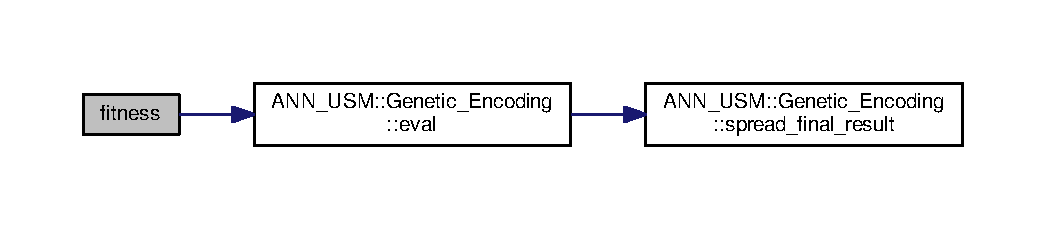
\includegraphics[width=350pt]{fitness_8hpp_ab547101b5cc5b5c2957842bea97514ce_cgraph}
\end{center}
\end{figure}




Here is the caller graph for this function\-:\nopagebreak
\begin{figure}[H]
\begin{center}
\leavevmode
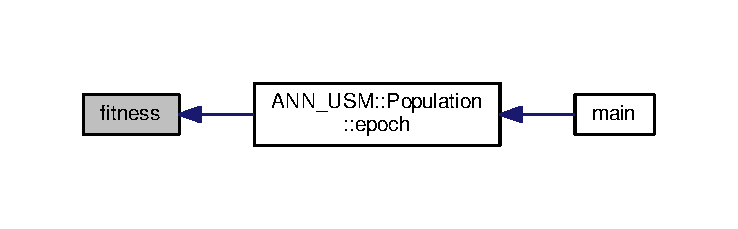
\includegraphics[width=350pt]{fitness_8hpp_ab547101b5cc5b5c2957842bea97514ce_icgraph}
\end{center}
\end{figure}



\hypertarget{function_8hpp}{\section{headers/function.hpp File Reference}
\label{function_8hpp}\index{headers/function.\-hpp@{headers/function.\-hpp}}
}
{\ttfamily \#include $<$cmath$>$}\\*
{\ttfamily \#include $<$string$>$}\\*
{\ttfamily \#include $<$vector$>$}\\*
Include dependency graph for function.\-hpp\-:
\nopagebreak
\begin{figure}[H]
\begin{center}
\leavevmode
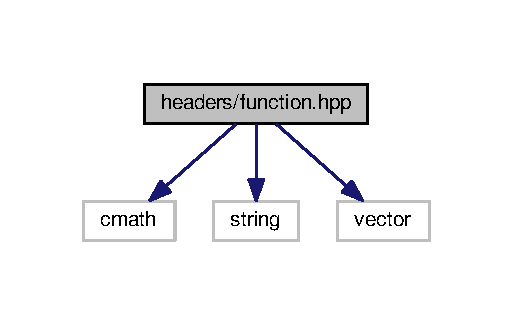
\includegraphics[width=246pt]{function_8hpp__incl}
\end{center}
\end{figure}
This graph shows which files directly or indirectly include this file\-:
\nopagebreak
\begin{figure}[H]
\begin{center}
\leavevmode
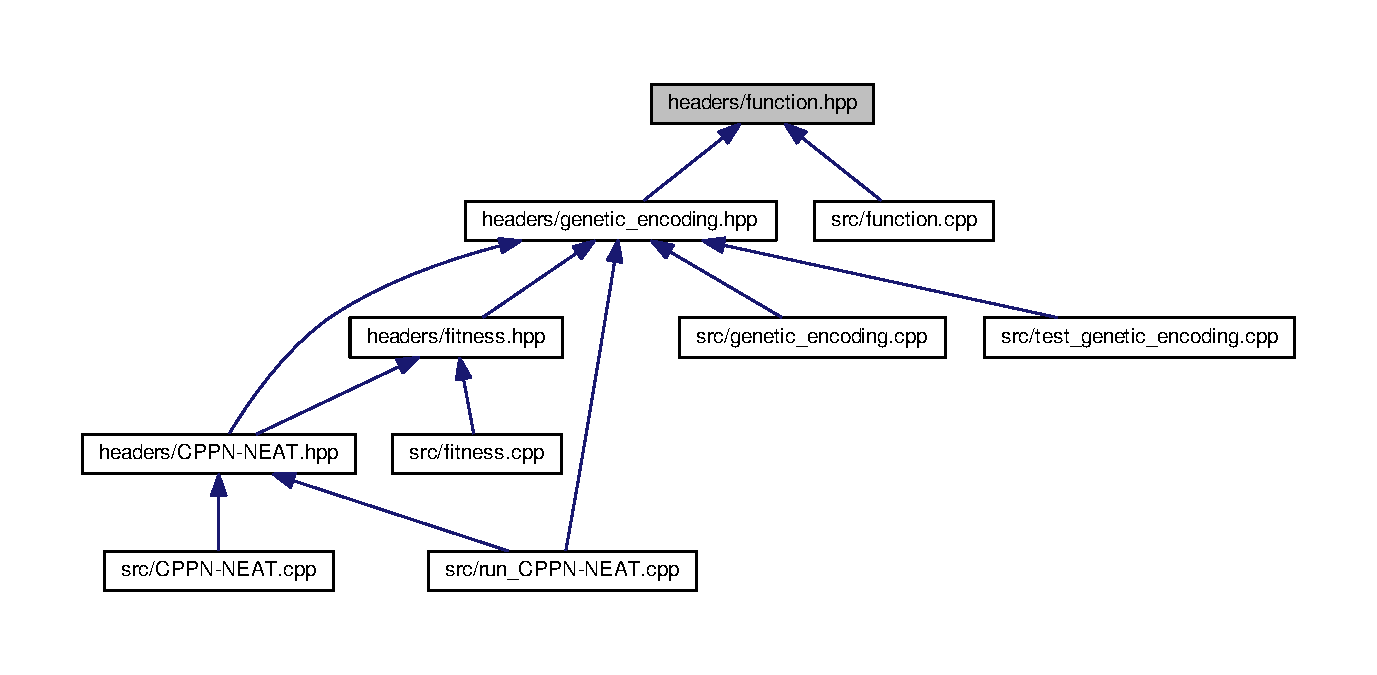
\includegraphics[width=350pt]{function_8hpp__dep__incl}
\end{center}
\end{figure}
\subsection*{Classes}
\begin{DoxyCompactItemize}
\item 
class \hyperlink{class_function}{Function}
\end{DoxyCompactItemize}

\hypertarget{genetic__encoding_8hpp}{\section{headers/genetic\-\_\-encoding.hpp File Reference}
\label{genetic__encoding_8hpp}\index{headers/genetic\-\_\-encoding.\-hpp@{headers/genetic\-\_\-encoding.\-hpp}}
}
{\ttfamily \#include $<$vector$>$}\\*
{\ttfamily \#include $<$cstdlib$>$}\\*
{\ttfamily \#include $<$iostream$>$}\\*
{\ttfamily \#include $<$string$>$}\\*
{\ttfamily \#include $<$sstream$>$}\\*
{\ttfamily \#include $<$fstream$>$}\\*
{\ttfamily \#include $<$strings.\-h$>$}\\*
{\ttfamily \#include \char`\"{}user\-\_\-definitions.\-hpp\char`\"{}}\\*
{\ttfamily \#include \char`\"{}function.\-hpp\char`\"{}}\\*
Include dependency graph for genetic\-\_\-encoding.\-hpp\-:
\nopagebreak
\begin{figure}[H]
\begin{center}
\leavevmode
\includegraphics[width=350pt]{genetic__encoding_8hpp__incl}
\end{center}
\end{figure}
This graph shows which files directly or indirectly include this file\-:
\nopagebreak
\begin{figure}[H]
\begin{center}
\leavevmode
\includegraphics[width=350pt]{genetic__encoding_8hpp__dep__incl}
\end{center}
\end{figure}
\subsection*{Classes}
\begin{DoxyCompactItemize}
\item 
class \hyperlink{class_a_n_n___u_s_m_1_1connection__gene}{A\-N\-N\-\_\-\-U\-S\-M\-::connection\-\_\-gene}
\item 
class \hyperlink{class_a_n_n___u_s_m_1_1node__gene}{A\-N\-N\-\_\-\-U\-S\-M\-::node\-\_\-gene}
\item 
class \hyperlink{class_a_n_n___u_s_m_1_1_genetic___encoding}{A\-N\-N\-\_\-\-U\-S\-M\-::\-Genetic\-\_\-\-Encoding}
\end{DoxyCompactItemize}
\subsection*{Namespaces}
\begin{DoxyCompactItemize}
\item 
\hyperlink{namespace_a_n_n___u_s_m}{A\-N\-N\-\_\-\-U\-S\-M}
\end{DoxyCompactItemize}
\subsection*{Enumerations}
\begin{DoxyCompactItemize}
\item 
enum \hyperlink{namespace_a_n_n___u_s_m_aa7f97f486244dd898592ba14dd7aa778}{A\-N\-N\-\_\-\-U\-S\-M\-::gene\-\_\-type} \{ \hyperlink{namespace_a_n_n___u_s_m_aa7f97f486244dd898592ba14dd7aa778a7d1709e4616ab876261529547517bd3d}{A\-N\-N\-\_\-\-U\-S\-M\-::\-I\-N\-P\-U\-T}, 
\hyperlink{namespace_a_n_n___u_s_m_aa7f97f486244dd898592ba14dd7aa778ac1f27e9ecf199fdd0f9c93c85c866e37}{A\-N\-N\-\_\-\-U\-S\-M\-::\-H\-I\-D\-D\-E\-N}, 
\hyperlink{namespace_a_n_n___u_s_m_aa7f97f486244dd898592ba14dd7aa778aef5e3b43b7a6121b9cd2bce132cf07b7}{A\-N\-N\-\_\-\-U\-S\-M\-::\-O\-U\-T\-P\-U\-T}
 \}
\end{DoxyCompactItemize}
\subsection*{Functions}
\begin{DoxyCompactItemize}
\item 
ostream \& \hyperlink{genetic__encoding_8hpp_a9adc11b1d1ef09e5f628a4506f2166ef}{operator$<$$<$} (ostream \&o, \hyperlink{class_a_n_n___u_s_m_1_1_genetic___encoding}{A\-N\-N\-\_\-\-U\-S\-M\-::\-Genetic\-\_\-\-Encoding} \&encoding)
\end{DoxyCompactItemize}


\subsection{Function Documentation}
\hypertarget{genetic__encoding_8hpp_a9adc11b1d1ef09e5f628a4506f2166ef}{\index{genetic\-\_\-encoding.\-hpp@{genetic\-\_\-encoding.\-hpp}!operator$<$$<$@{operator$<$$<$}}
\index{operator$<$$<$@{operator$<$$<$}!genetic_encoding.hpp@{genetic\-\_\-encoding.\-hpp}}
\subsubsection[{operator$<$$<$}]{\setlength{\rightskip}{0pt plus 5cm}ostream\& operator$<$$<$ (
\begin{DoxyParamCaption}
\item[{ostream \&}]{o, }
\item[{{\bf A\-N\-N\-\_\-\-U\-S\-M\-::\-Genetic\-\_\-\-Encoding} \&}]{encoding}
\end{DoxyParamCaption}
)}}\label{genetic__encoding_8hpp_a9adc11b1d1ef09e5f628a4506f2166ef}


Definition at line 391 of file genetic\-\_\-encoding.\-cpp.



Here is the call graph for this function\-:\nopagebreak
\begin{figure}[H]
\begin{center}
\leavevmode
\includegraphics[width=332pt]{genetic__encoding_8hpp_a9adc11b1d1ef09e5f628a4506f2166ef_cgraph}
\end{center}
\end{figure}



\hypertarget{user__definitions_8hpp}{\section{headers/user\-\_\-definitions.hpp File Reference}
\label{user__definitions_8hpp}\index{headers/user\-\_\-definitions.\-hpp@{headers/user\-\_\-definitions.\-hpp}}
}
This graph shows which files directly or indirectly include this file\-:
\nopagebreak
\begin{figure}[H]
\begin{center}
\leavevmode
\includegraphics[width=350pt]{user__definitions_8hpp__dep__incl}
\end{center}
\end{figure}
\subsection*{Macros}
\begin{DoxyCompactItemize}
\item 
\#define \hyperlink{user__definitions_8hpp_ab57a8793e8afbbd82d1f47aa5bb16470}{P\-O\-P\-U\-L\-A\-T\-I\-O\-N\-\_\-\-M\-A\-X}~150
\item 
\#define \hyperlink{user__definitions_8hpp_a75bfaadb929713fba64ee5f798a4f334}{D\-I\-S\-T\-A\-N\-C\-E\-\_\-\-C\-O\-N\-S\-T\-\_\-1}~1.\-0
\item 
\#define \hyperlink{user__definitions_8hpp_a265b98f29b3f8fc0ccb275170361a3f7}{D\-I\-S\-T\-A\-N\-C\-E\-\_\-\-C\-O\-N\-S\-T\-\_\-2}~0.\-4
\item 
\#define \hyperlink{user__definitions_8hpp_a4867921f73a177a2147ef3b1daf28103}{D\-I\-S\-T\-A\-N\-C\-E\-\_\-\-C\-O\-N\-S\-T\-\_\-3}~1.\-0
\item 
\#define \hyperlink{user__definitions_8hpp_aadbb2284310c02e98d258265703e7f32}{D\-I\-S\-T\-A\-N\-C\-E\-\_\-\-C\-O\-N\-S\-T\-\_\-4}~1.\-0
\item 
\#define \hyperlink{user__definitions_8hpp_a00719a0387f578831fd8b092bd4d38d3}{D\-I\-S\-T\-A\-N\-C\-E\-\_\-\-T\-H\-R\-E\-S\-H\-O\-L\-D}~3.\-0
\item 
\#define \hyperlink{user__definitions_8hpp_a4a89e64438d0aedde56f521bed8bcf76}{P\-E\-R\-C\-E\-N\-T\-\_\-\-M\-U\-T\-A\-T\-I\-O\-N\-\_\-\-C\-O\-N\-N\-E\-C\-T\-I\-O\-N}~0.\-25
\item 
\#define \hyperlink{user__definitions_8hpp_a0ebce6100664b49d2f7149870fc32ccc}{P\-E\-R\-C\-E\-N\-T\-A\-G\-E\-\_\-\-O\-F\-F\-S\-P\-R\-I\-N\-G\-\_\-\-W\-I\-T\-H\-O\-U\-T\-\_\-\-C\-R\-O\-S\-S\-O\-V\-E\-R}~25
\item 
\#define \hyperlink{user__definitions_8hpp_a1e8230d3ae8d2e88cdf2257c98a05afe}{P\-R\-O\-B\-A\-B\-I\-L\-I\-T\-Y\-\_\-\-I\-N\-T\-E\-R\-S\-P\-A\-C\-I\-E\-S\-\_\-\-M\-A\-T\-I\-N\-G}~0.\-01
\item 
\#define \hyperlink{user__definitions_8hpp_ae3fc0f666189b4c801a004d220448d64}{S\-M\-A\-L\-L\-E\-R\-\_\-\-P\-O\-P\-U\-L\-A\-T\-I\-O\-N\-S\-\_\-\-P\-R\-O\-B\-A\-B\-I\-L\-I\-T\-Y\-\_\-\-A\-D\-D\-I\-N\-G\-\_\-\-N\-E\-W\-\_\-\-N\-O\-D\-E}~0.\-07
\item 
\#define \hyperlink{user__definitions_8hpp_a8442c433b0aa7122ae9cf32231861673}{S\-M\-A\-L\-L\-E\-R\-\_\-\-P\-O\-P\-U\-L\-A\-T\-I\-O\-N\-S\-\_\-\-P\-R\-O\-B\-A\-B\-I\-L\-I\-T\-Y\-\_\-\-A\-D\-D\-I\-N\-G\-\_\-\-N\-E\-W\-\_\-\-C\-O\-N\-N\-E\-C\-T\-I\-O\-N}~0.\-05
\item 
\#define \hyperlink{user__definitions_8hpp_ac7e9919db3c744e183ef2e2ea3fc6bed}{L\-A\-R\-G\-E\-R\-\_\-\-P\-O\-P\-U\-L\-A\-T\-I\-O\-N\-S\-\_\-\-P\-R\-O\-B\-A\-B\-I\-L\-I\-T\-Y\-\_\-\-A\-D\-D\-I\-N\-G\-\_\-\-N\-E\-W\-\_\-\-N\-O\-D\-E}~0.\-01
\item 
\#define \hyperlink{user__definitions_8hpp_ab2d7e06916788e675fc701e81f86de9d}{L\-A\-R\-G\-E\-R\-\_\-\-P\-O\-P\-U\-L\-A\-T\-I\-O\-N\-S\-\_\-\-P\-R\-O\-B\-A\-B\-I\-L\-I\-T\-Y\-\_\-\-A\-D\-D\-I\-N\-G\-\_\-\-N\-E\-W\-\_\-\-C\-O\-N\-N\-E\-C\-T\-I\-O\-N}~0.\-3
\item 
\#define \hyperlink{user__definitions_8hpp_af75785771a98007c6c7f9bb364c5aa2c}{P\-R\-O\-B\-A\-B\-I\-L\-I\-T\-Y\-\_\-\-C\-O\-N\-N\-E\-C\-T\-I\-O\-N\-\_\-\-W\-E\-I\-G\-H\-T\-\_\-\-M\-U\-T\-A\-T\-I\-N\-G}~80
\item 
\#define \hyperlink{user__definitions_8hpp_ae7f1d69a2ba1478659f40b346b46cd00}{L\-A\-R\-G\-E\-\_\-\-P\-O\-P\-U\-L\-A\-T\-I\-O\-N\-\_\-\-D\-I\-S\-C\-R\-I\-M\-I\-N\-A\-T\-O\-R}~(\hyperlink{user__definitions_8hpp_ab57a8793e8afbbd82d1f47aa5bb16470}{P\-O\-P\-U\-L\-A\-T\-I\-O\-N\-\_\-\-M\-A\-X}/10.\-0)
\item 
\#define \hyperlink{user__definitions_8hpp_a72f33a4bf5f6d9630f61ed83a7514fde}{F\-U\-N\-C\-T\-I\-O\-N\-\_\-\-N\-U\-M}~6
\item 
\#define \hyperlink{user__definitions_8hpp_a516d0c5670fad64f0c2d47a893c695a4}{G\-E\-N\-E\-R\-A\-T\-I\-O\-N\-S}~50
\end{DoxyCompactItemize}


\subsection{Macro Definition Documentation}
\hypertarget{user__definitions_8hpp_a75bfaadb929713fba64ee5f798a4f334}{\index{user\-\_\-definitions.\-hpp@{user\-\_\-definitions.\-hpp}!D\-I\-S\-T\-A\-N\-C\-E\-\_\-\-C\-O\-N\-S\-T\-\_\-1@{D\-I\-S\-T\-A\-N\-C\-E\-\_\-\-C\-O\-N\-S\-T\-\_\-1}}
\index{D\-I\-S\-T\-A\-N\-C\-E\-\_\-\-C\-O\-N\-S\-T\-\_\-1@{D\-I\-S\-T\-A\-N\-C\-E\-\_\-\-C\-O\-N\-S\-T\-\_\-1}!user_definitions.hpp@{user\-\_\-definitions.\-hpp}}
\subsubsection[{D\-I\-S\-T\-A\-N\-C\-E\-\_\-\-C\-O\-N\-S\-T\-\_\-1}]{\setlength{\rightskip}{0pt plus 5cm}\#define D\-I\-S\-T\-A\-N\-C\-E\-\_\-\-C\-O\-N\-S\-T\-\_\-1~1.\-0}}\label{user__definitions_8hpp_a75bfaadb929713fba64ee5f798a4f334}


Definition at line 6 of file user\-\_\-definitions.\-hpp.

\hypertarget{user__definitions_8hpp_a265b98f29b3f8fc0ccb275170361a3f7}{\index{user\-\_\-definitions.\-hpp@{user\-\_\-definitions.\-hpp}!D\-I\-S\-T\-A\-N\-C\-E\-\_\-\-C\-O\-N\-S\-T\-\_\-2@{D\-I\-S\-T\-A\-N\-C\-E\-\_\-\-C\-O\-N\-S\-T\-\_\-2}}
\index{D\-I\-S\-T\-A\-N\-C\-E\-\_\-\-C\-O\-N\-S\-T\-\_\-2@{D\-I\-S\-T\-A\-N\-C\-E\-\_\-\-C\-O\-N\-S\-T\-\_\-2}!user_definitions.hpp@{user\-\_\-definitions.\-hpp}}
\subsubsection[{D\-I\-S\-T\-A\-N\-C\-E\-\_\-\-C\-O\-N\-S\-T\-\_\-2}]{\setlength{\rightskip}{0pt plus 5cm}\#define D\-I\-S\-T\-A\-N\-C\-E\-\_\-\-C\-O\-N\-S\-T\-\_\-2~0.\-4}}\label{user__definitions_8hpp_a265b98f29b3f8fc0ccb275170361a3f7}


Definition at line 7 of file user\-\_\-definitions.\-hpp.

\hypertarget{user__definitions_8hpp_a4867921f73a177a2147ef3b1daf28103}{\index{user\-\_\-definitions.\-hpp@{user\-\_\-definitions.\-hpp}!D\-I\-S\-T\-A\-N\-C\-E\-\_\-\-C\-O\-N\-S\-T\-\_\-3@{D\-I\-S\-T\-A\-N\-C\-E\-\_\-\-C\-O\-N\-S\-T\-\_\-3}}
\index{D\-I\-S\-T\-A\-N\-C\-E\-\_\-\-C\-O\-N\-S\-T\-\_\-3@{D\-I\-S\-T\-A\-N\-C\-E\-\_\-\-C\-O\-N\-S\-T\-\_\-3}!user_definitions.hpp@{user\-\_\-definitions.\-hpp}}
\subsubsection[{D\-I\-S\-T\-A\-N\-C\-E\-\_\-\-C\-O\-N\-S\-T\-\_\-3}]{\setlength{\rightskip}{0pt plus 5cm}\#define D\-I\-S\-T\-A\-N\-C\-E\-\_\-\-C\-O\-N\-S\-T\-\_\-3~1.\-0}}\label{user__definitions_8hpp_a4867921f73a177a2147ef3b1daf28103}


Definition at line 8 of file user\-\_\-definitions.\-hpp.

\hypertarget{user__definitions_8hpp_aadbb2284310c02e98d258265703e7f32}{\index{user\-\_\-definitions.\-hpp@{user\-\_\-definitions.\-hpp}!D\-I\-S\-T\-A\-N\-C\-E\-\_\-\-C\-O\-N\-S\-T\-\_\-4@{D\-I\-S\-T\-A\-N\-C\-E\-\_\-\-C\-O\-N\-S\-T\-\_\-4}}
\index{D\-I\-S\-T\-A\-N\-C\-E\-\_\-\-C\-O\-N\-S\-T\-\_\-4@{D\-I\-S\-T\-A\-N\-C\-E\-\_\-\-C\-O\-N\-S\-T\-\_\-4}!user_definitions.hpp@{user\-\_\-definitions.\-hpp}}
\subsubsection[{D\-I\-S\-T\-A\-N\-C\-E\-\_\-\-C\-O\-N\-S\-T\-\_\-4}]{\setlength{\rightskip}{0pt plus 5cm}\#define D\-I\-S\-T\-A\-N\-C\-E\-\_\-\-C\-O\-N\-S\-T\-\_\-4~1.\-0}}\label{user__definitions_8hpp_aadbb2284310c02e98d258265703e7f32}


Definition at line 9 of file user\-\_\-definitions.\-hpp.

\hypertarget{user__definitions_8hpp_a00719a0387f578831fd8b092bd4d38d3}{\index{user\-\_\-definitions.\-hpp@{user\-\_\-definitions.\-hpp}!D\-I\-S\-T\-A\-N\-C\-E\-\_\-\-T\-H\-R\-E\-S\-H\-O\-L\-D@{D\-I\-S\-T\-A\-N\-C\-E\-\_\-\-T\-H\-R\-E\-S\-H\-O\-L\-D}}
\index{D\-I\-S\-T\-A\-N\-C\-E\-\_\-\-T\-H\-R\-E\-S\-H\-O\-L\-D@{D\-I\-S\-T\-A\-N\-C\-E\-\_\-\-T\-H\-R\-E\-S\-H\-O\-L\-D}!user_definitions.hpp@{user\-\_\-definitions.\-hpp}}
\subsubsection[{D\-I\-S\-T\-A\-N\-C\-E\-\_\-\-T\-H\-R\-E\-S\-H\-O\-L\-D}]{\setlength{\rightskip}{0pt plus 5cm}\#define D\-I\-S\-T\-A\-N\-C\-E\-\_\-\-T\-H\-R\-E\-S\-H\-O\-L\-D~3.\-0}}\label{user__definitions_8hpp_a00719a0387f578831fd8b092bd4d38d3}


Definition at line 10 of file user\-\_\-definitions.\-hpp.

\hypertarget{user__definitions_8hpp_a72f33a4bf5f6d9630f61ed83a7514fde}{\index{user\-\_\-definitions.\-hpp@{user\-\_\-definitions.\-hpp}!F\-U\-N\-C\-T\-I\-O\-N\-\_\-\-N\-U\-M@{F\-U\-N\-C\-T\-I\-O\-N\-\_\-\-N\-U\-M}}
\index{F\-U\-N\-C\-T\-I\-O\-N\-\_\-\-N\-U\-M@{F\-U\-N\-C\-T\-I\-O\-N\-\_\-\-N\-U\-M}!user_definitions.hpp@{user\-\_\-definitions.\-hpp}}
\subsubsection[{F\-U\-N\-C\-T\-I\-O\-N\-\_\-\-N\-U\-M}]{\setlength{\rightskip}{0pt plus 5cm}\#define F\-U\-N\-C\-T\-I\-O\-N\-\_\-\-N\-U\-M~6}}\label{user__definitions_8hpp_a72f33a4bf5f6d9630f61ed83a7514fde}


Definition at line 22 of file user\-\_\-definitions.\-hpp.

\hypertarget{user__definitions_8hpp_a516d0c5670fad64f0c2d47a893c695a4}{\index{user\-\_\-definitions.\-hpp@{user\-\_\-definitions.\-hpp}!G\-E\-N\-E\-R\-A\-T\-I\-O\-N\-S@{G\-E\-N\-E\-R\-A\-T\-I\-O\-N\-S}}
\index{G\-E\-N\-E\-R\-A\-T\-I\-O\-N\-S@{G\-E\-N\-E\-R\-A\-T\-I\-O\-N\-S}!user_definitions.hpp@{user\-\_\-definitions.\-hpp}}
\subsubsection[{G\-E\-N\-E\-R\-A\-T\-I\-O\-N\-S}]{\setlength{\rightskip}{0pt plus 5cm}\#define G\-E\-N\-E\-R\-A\-T\-I\-O\-N\-S~50}}\label{user__definitions_8hpp_a516d0c5670fad64f0c2d47a893c695a4}


Definition at line 23 of file user\-\_\-definitions.\-hpp.

\hypertarget{user__definitions_8hpp_ae7f1d69a2ba1478659f40b346b46cd00}{\index{user\-\_\-definitions.\-hpp@{user\-\_\-definitions.\-hpp}!L\-A\-R\-G\-E\-\_\-\-P\-O\-P\-U\-L\-A\-T\-I\-O\-N\-\_\-\-D\-I\-S\-C\-R\-I\-M\-I\-N\-A\-T\-O\-R@{L\-A\-R\-G\-E\-\_\-\-P\-O\-P\-U\-L\-A\-T\-I\-O\-N\-\_\-\-D\-I\-S\-C\-R\-I\-M\-I\-N\-A\-T\-O\-R}}
\index{L\-A\-R\-G\-E\-\_\-\-P\-O\-P\-U\-L\-A\-T\-I\-O\-N\-\_\-\-D\-I\-S\-C\-R\-I\-M\-I\-N\-A\-T\-O\-R@{L\-A\-R\-G\-E\-\_\-\-P\-O\-P\-U\-L\-A\-T\-I\-O\-N\-\_\-\-D\-I\-S\-C\-R\-I\-M\-I\-N\-A\-T\-O\-R}!user_definitions.hpp@{user\-\_\-definitions.\-hpp}}
\subsubsection[{L\-A\-R\-G\-E\-\_\-\-P\-O\-P\-U\-L\-A\-T\-I\-O\-N\-\_\-\-D\-I\-S\-C\-R\-I\-M\-I\-N\-A\-T\-O\-R}]{\setlength{\rightskip}{0pt plus 5cm}\#define L\-A\-R\-G\-E\-\_\-\-P\-O\-P\-U\-L\-A\-T\-I\-O\-N\-\_\-\-D\-I\-S\-C\-R\-I\-M\-I\-N\-A\-T\-O\-R~({\bf P\-O\-P\-U\-L\-A\-T\-I\-O\-N\-\_\-\-M\-A\-X}/10.\-0)}}\label{user__definitions_8hpp_ae7f1d69a2ba1478659f40b346b46cd00}


Definition at line 20 of file user\-\_\-definitions.\-hpp.

\hypertarget{user__definitions_8hpp_ab2d7e06916788e675fc701e81f86de9d}{\index{user\-\_\-definitions.\-hpp@{user\-\_\-definitions.\-hpp}!L\-A\-R\-G\-E\-R\-\_\-\-P\-O\-P\-U\-L\-A\-T\-I\-O\-N\-S\-\_\-\-P\-R\-O\-B\-A\-B\-I\-L\-I\-T\-Y\-\_\-\-A\-D\-D\-I\-N\-G\-\_\-\-N\-E\-W\-\_\-\-C\-O\-N\-N\-E\-C\-T\-I\-O\-N@{L\-A\-R\-G\-E\-R\-\_\-\-P\-O\-P\-U\-L\-A\-T\-I\-O\-N\-S\-\_\-\-P\-R\-O\-B\-A\-B\-I\-L\-I\-T\-Y\-\_\-\-A\-D\-D\-I\-N\-G\-\_\-\-N\-E\-W\-\_\-\-C\-O\-N\-N\-E\-C\-T\-I\-O\-N}}
\index{L\-A\-R\-G\-E\-R\-\_\-\-P\-O\-P\-U\-L\-A\-T\-I\-O\-N\-S\-\_\-\-P\-R\-O\-B\-A\-B\-I\-L\-I\-T\-Y\-\_\-\-A\-D\-D\-I\-N\-G\-\_\-\-N\-E\-W\-\_\-\-C\-O\-N\-N\-E\-C\-T\-I\-O\-N@{L\-A\-R\-G\-E\-R\-\_\-\-P\-O\-P\-U\-L\-A\-T\-I\-O\-N\-S\-\_\-\-P\-R\-O\-B\-A\-B\-I\-L\-I\-T\-Y\-\_\-\-A\-D\-D\-I\-N\-G\-\_\-\-N\-E\-W\-\_\-\-C\-O\-N\-N\-E\-C\-T\-I\-O\-N}!user_definitions.hpp@{user\-\_\-definitions.\-hpp}}
\subsubsection[{L\-A\-R\-G\-E\-R\-\_\-\-P\-O\-P\-U\-L\-A\-T\-I\-O\-N\-S\-\_\-\-P\-R\-O\-B\-A\-B\-I\-L\-I\-T\-Y\-\_\-\-A\-D\-D\-I\-N\-G\-\_\-\-N\-E\-W\-\_\-\-C\-O\-N\-N\-E\-C\-T\-I\-O\-N}]{\setlength{\rightskip}{0pt plus 5cm}\#define L\-A\-R\-G\-E\-R\-\_\-\-P\-O\-P\-U\-L\-A\-T\-I\-O\-N\-S\-\_\-\-P\-R\-O\-B\-A\-B\-I\-L\-I\-T\-Y\-\_\-\-A\-D\-D\-I\-N\-G\-\_\-\-N\-E\-W\-\_\-\-C\-O\-N\-N\-E\-C\-T\-I\-O\-N~0.\-3}}\label{user__definitions_8hpp_ab2d7e06916788e675fc701e81f86de9d}


Definition at line 18 of file user\-\_\-definitions.\-hpp.

\hypertarget{user__definitions_8hpp_ac7e9919db3c744e183ef2e2ea3fc6bed}{\index{user\-\_\-definitions.\-hpp@{user\-\_\-definitions.\-hpp}!L\-A\-R\-G\-E\-R\-\_\-\-P\-O\-P\-U\-L\-A\-T\-I\-O\-N\-S\-\_\-\-P\-R\-O\-B\-A\-B\-I\-L\-I\-T\-Y\-\_\-\-A\-D\-D\-I\-N\-G\-\_\-\-N\-E\-W\-\_\-\-N\-O\-D\-E@{L\-A\-R\-G\-E\-R\-\_\-\-P\-O\-P\-U\-L\-A\-T\-I\-O\-N\-S\-\_\-\-P\-R\-O\-B\-A\-B\-I\-L\-I\-T\-Y\-\_\-\-A\-D\-D\-I\-N\-G\-\_\-\-N\-E\-W\-\_\-\-N\-O\-D\-E}}
\index{L\-A\-R\-G\-E\-R\-\_\-\-P\-O\-P\-U\-L\-A\-T\-I\-O\-N\-S\-\_\-\-P\-R\-O\-B\-A\-B\-I\-L\-I\-T\-Y\-\_\-\-A\-D\-D\-I\-N\-G\-\_\-\-N\-E\-W\-\_\-\-N\-O\-D\-E@{L\-A\-R\-G\-E\-R\-\_\-\-P\-O\-P\-U\-L\-A\-T\-I\-O\-N\-S\-\_\-\-P\-R\-O\-B\-A\-B\-I\-L\-I\-T\-Y\-\_\-\-A\-D\-D\-I\-N\-G\-\_\-\-N\-E\-W\-\_\-\-N\-O\-D\-E}!user_definitions.hpp@{user\-\_\-definitions.\-hpp}}
\subsubsection[{L\-A\-R\-G\-E\-R\-\_\-\-P\-O\-P\-U\-L\-A\-T\-I\-O\-N\-S\-\_\-\-P\-R\-O\-B\-A\-B\-I\-L\-I\-T\-Y\-\_\-\-A\-D\-D\-I\-N\-G\-\_\-\-N\-E\-W\-\_\-\-N\-O\-D\-E}]{\setlength{\rightskip}{0pt plus 5cm}\#define L\-A\-R\-G\-E\-R\-\_\-\-P\-O\-P\-U\-L\-A\-T\-I\-O\-N\-S\-\_\-\-P\-R\-O\-B\-A\-B\-I\-L\-I\-T\-Y\-\_\-\-A\-D\-D\-I\-N\-G\-\_\-\-N\-E\-W\-\_\-\-N\-O\-D\-E~0.\-01}}\label{user__definitions_8hpp_ac7e9919db3c744e183ef2e2ea3fc6bed}


Definition at line 17 of file user\-\_\-definitions.\-hpp.

\hypertarget{user__definitions_8hpp_a4a89e64438d0aedde56f521bed8bcf76}{\index{user\-\_\-definitions.\-hpp@{user\-\_\-definitions.\-hpp}!P\-E\-R\-C\-E\-N\-T\-\_\-\-M\-U\-T\-A\-T\-I\-O\-N\-\_\-\-C\-O\-N\-N\-E\-C\-T\-I\-O\-N@{P\-E\-R\-C\-E\-N\-T\-\_\-\-M\-U\-T\-A\-T\-I\-O\-N\-\_\-\-C\-O\-N\-N\-E\-C\-T\-I\-O\-N}}
\index{P\-E\-R\-C\-E\-N\-T\-\_\-\-M\-U\-T\-A\-T\-I\-O\-N\-\_\-\-C\-O\-N\-N\-E\-C\-T\-I\-O\-N@{P\-E\-R\-C\-E\-N\-T\-\_\-\-M\-U\-T\-A\-T\-I\-O\-N\-\_\-\-C\-O\-N\-N\-E\-C\-T\-I\-O\-N}!user_definitions.hpp@{user\-\_\-definitions.\-hpp}}
\subsubsection[{P\-E\-R\-C\-E\-N\-T\-\_\-\-M\-U\-T\-A\-T\-I\-O\-N\-\_\-\-C\-O\-N\-N\-E\-C\-T\-I\-O\-N}]{\setlength{\rightskip}{0pt plus 5cm}\#define P\-E\-R\-C\-E\-N\-T\-\_\-\-M\-U\-T\-A\-T\-I\-O\-N\-\_\-\-C\-O\-N\-N\-E\-C\-T\-I\-O\-N~0.\-25}}\label{user__definitions_8hpp_a4a89e64438d0aedde56f521bed8bcf76}


Definition at line 12 of file user\-\_\-definitions.\-hpp.

\hypertarget{user__definitions_8hpp_a0ebce6100664b49d2f7149870fc32ccc}{\index{user\-\_\-definitions.\-hpp@{user\-\_\-definitions.\-hpp}!P\-E\-R\-C\-E\-N\-T\-A\-G\-E\-\_\-\-O\-F\-F\-S\-P\-R\-I\-N\-G\-\_\-\-W\-I\-T\-H\-O\-U\-T\-\_\-\-C\-R\-O\-S\-S\-O\-V\-E\-R@{P\-E\-R\-C\-E\-N\-T\-A\-G\-E\-\_\-\-O\-F\-F\-S\-P\-R\-I\-N\-G\-\_\-\-W\-I\-T\-H\-O\-U\-T\-\_\-\-C\-R\-O\-S\-S\-O\-V\-E\-R}}
\index{P\-E\-R\-C\-E\-N\-T\-A\-G\-E\-\_\-\-O\-F\-F\-S\-P\-R\-I\-N\-G\-\_\-\-W\-I\-T\-H\-O\-U\-T\-\_\-\-C\-R\-O\-S\-S\-O\-V\-E\-R@{P\-E\-R\-C\-E\-N\-T\-A\-G\-E\-\_\-\-O\-F\-F\-S\-P\-R\-I\-N\-G\-\_\-\-W\-I\-T\-H\-O\-U\-T\-\_\-\-C\-R\-O\-S\-S\-O\-V\-E\-R}!user_definitions.hpp@{user\-\_\-definitions.\-hpp}}
\subsubsection[{P\-E\-R\-C\-E\-N\-T\-A\-G\-E\-\_\-\-O\-F\-F\-S\-P\-R\-I\-N\-G\-\_\-\-W\-I\-T\-H\-O\-U\-T\-\_\-\-C\-R\-O\-S\-S\-O\-V\-E\-R}]{\setlength{\rightskip}{0pt plus 5cm}\#define P\-E\-R\-C\-E\-N\-T\-A\-G\-E\-\_\-\-O\-F\-F\-S\-P\-R\-I\-N\-G\-\_\-\-W\-I\-T\-H\-O\-U\-T\-\_\-\-C\-R\-O\-S\-S\-O\-V\-E\-R~25}}\label{user__definitions_8hpp_a0ebce6100664b49d2f7149870fc32ccc}


Definition at line 13 of file user\-\_\-definitions.\-hpp.

\hypertarget{user__definitions_8hpp_ab57a8793e8afbbd82d1f47aa5bb16470}{\index{user\-\_\-definitions.\-hpp@{user\-\_\-definitions.\-hpp}!P\-O\-P\-U\-L\-A\-T\-I\-O\-N\-\_\-\-M\-A\-X@{P\-O\-P\-U\-L\-A\-T\-I\-O\-N\-\_\-\-M\-A\-X}}
\index{P\-O\-P\-U\-L\-A\-T\-I\-O\-N\-\_\-\-M\-A\-X@{P\-O\-P\-U\-L\-A\-T\-I\-O\-N\-\_\-\-M\-A\-X}!user_definitions.hpp@{user\-\_\-definitions.\-hpp}}
\subsubsection[{P\-O\-P\-U\-L\-A\-T\-I\-O\-N\-\_\-\-M\-A\-X}]{\setlength{\rightskip}{0pt plus 5cm}\#define P\-O\-P\-U\-L\-A\-T\-I\-O\-N\-\_\-\-M\-A\-X~150}}\label{user__definitions_8hpp_ab57a8793e8afbbd82d1f47aa5bb16470}


Definition at line 5 of file user\-\_\-definitions.\-hpp.

\hypertarget{user__definitions_8hpp_af75785771a98007c6c7f9bb364c5aa2c}{\index{user\-\_\-definitions.\-hpp@{user\-\_\-definitions.\-hpp}!P\-R\-O\-B\-A\-B\-I\-L\-I\-T\-Y\-\_\-\-C\-O\-N\-N\-E\-C\-T\-I\-O\-N\-\_\-\-W\-E\-I\-G\-H\-T\-\_\-\-M\-U\-T\-A\-T\-I\-N\-G@{P\-R\-O\-B\-A\-B\-I\-L\-I\-T\-Y\-\_\-\-C\-O\-N\-N\-E\-C\-T\-I\-O\-N\-\_\-\-W\-E\-I\-G\-H\-T\-\_\-\-M\-U\-T\-A\-T\-I\-N\-G}}
\index{P\-R\-O\-B\-A\-B\-I\-L\-I\-T\-Y\-\_\-\-C\-O\-N\-N\-E\-C\-T\-I\-O\-N\-\_\-\-W\-E\-I\-G\-H\-T\-\_\-\-M\-U\-T\-A\-T\-I\-N\-G@{P\-R\-O\-B\-A\-B\-I\-L\-I\-T\-Y\-\_\-\-C\-O\-N\-N\-E\-C\-T\-I\-O\-N\-\_\-\-W\-E\-I\-G\-H\-T\-\_\-\-M\-U\-T\-A\-T\-I\-N\-G}!user_definitions.hpp@{user\-\_\-definitions.\-hpp}}
\subsubsection[{P\-R\-O\-B\-A\-B\-I\-L\-I\-T\-Y\-\_\-\-C\-O\-N\-N\-E\-C\-T\-I\-O\-N\-\_\-\-W\-E\-I\-G\-H\-T\-\_\-\-M\-U\-T\-A\-T\-I\-N\-G}]{\setlength{\rightskip}{0pt plus 5cm}\#define P\-R\-O\-B\-A\-B\-I\-L\-I\-T\-Y\-\_\-\-C\-O\-N\-N\-E\-C\-T\-I\-O\-N\-\_\-\-W\-E\-I\-G\-H\-T\-\_\-\-M\-U\-T\-A\-T\-I\-N\-G~80}}\label{user__definitions_8hpp_af75785771a98007c6c7f9bb364c5aa2c}


Definition at line 19 of file user\-\_\-definitions.\-hpp.

\hypertarget{user__definitions_8hpp_a1e8230d3ae8d2e88cdf2257c98a05afe}{\index{user\-\_\-definitions.\-hpp@{user\-\_\-definitions.\-hpp}!P\-R\-O\-B\-A\-B\-I\-L\-I\-T\-Y\-\_\-\-I\-N\-T\-E\-R\-S\-P\-A\-C\-I\-E\-S\-\_\-\-M\-A\-T\-I\-N\-G@{P\-R\-O\-B\-A\-B\-I\-L\-I\-T\-Y\-\_\-\-I\-N\-T\-E\-R\-S\-P\-A\-C\-I\-E\-S\-\_\-\-M\-A\-T\-I\-N\-G}}
\index{P\-R\-O\-B\-A\-B\-I\-L\-I\-T\-Y\-\_\-\-I\-N\-T\-E\-R\-S\-P\-A\-C\-I\-E\-S\-\_\-\-M\-A\-T\-I\-N\-G@{P\-R\-O\-B\-A\-B\-I\-L\-I\-T\-Y\-\_\-\-I\-N\-T\-E\-R\-S\-P\-A\-C\-I\-E\-S\-\_\-\-M\-A\-T\-I\-N\-G}!user_definitions.hpp@{user\-\_\-definitions.\-hpp}}
\subsubsection[{P\-R\-O\-B\-A\-B\-I\-L\-I\-T\-Y\-\_\-\-I\-N\-T\-E\-R\-S\-P\-A\-C\-I\-E\-S\-\_\-\-M\-A\-T\-I\-N\-G}]{\setlength{\rightskip}{0pt plus 5cm}\#define P\-R\-O\-B\-A\-B\-I\-L\-I\-T\-Y\-\_\-\-I\-N\-T\-E\-R\-S\-P\-A\-C\-I\-E\-S\-\_\-\-M\-A\-T\-I\-N\-G~0.\-01}}\label{user__definitions_8hpp_a1e8230d3ae8d2e88cdf2257c98a05afe}


Definition at line 14 of file user\-\_\-definitions.\-hpp.

\hypertarget{user__definitions_8hpp_a8442c433b0aa7122ae9cf32231861673}{\index{user\-\_\-definitions.\-hpp@{user\-\_\-definitions.\-hpp}!S\-M\-A\-L\-L\-E\-R\-\_\-\-P\-O\-P\-U\-L\-A\-T\-I\-O\-N\-S\-\_\-\-P\-R\-O\-B\-A\-B\-I\-L\-I\-T\-Y\-\_\-\-A\-D\-D\-I\-N\-G\-\_\-\-N\-E\-W\-\_\-\-C\-O\-N\-N\-E\-C\-T\-I\-O\-N@{S\-M\-A\-L\-L\-E\-R\-\_\-\-P\-O\-P\-U\-L\-A\-T\-I\-O\-N\-S\-\_\-\-P\-R\-O\-B\-A\-B\-I\-L\-I\-T\-Y\-\_\-\-A\-D\-D\-I\-N\-G\-\_\-\-N\-E\-W\-\_\-\-C\-O\-N\-N\-E\-C\-T\-I\-O\-N}}
\index{S\-M\-A\-L\-L\-E\-R\-\_\-\-P\-O\-P\-U\-L\-A\-T\-I\-O\-N\-S\-\_\-\-P\-R\-O\-B\-A\-B\-I\-L\-I\-T\-Y\-\_\-\-A\-D\-D\-I\-N\-G\-\_\-\-N\-E\-W\-\_\-\-C\-O\-N\-N\-E\-C\-T\-I\-O\-N@{S\-M\-A\-L\-L\-E\-R\-\_\-\-P\-O\-P\-U\-L\-A\-T\-I\-O\-N\-S\-\_\-\-P\-R\-O\-B\-A\-B\-I\-L\-I\-T\-Y\-\_\-\-A\-D\-D\-I\-N\-G\-\_\-\-N\-E\-W\-\_\-\-C\-O\-N\-N\-E\-C\-T\-I\-O\-N}!user_definitions.hpp@{user\-\_\-definitions.\-hpp}}
\subsubsection[{S\-M\-A\-L\-L\-E\-R\-\_\-\-P\-O\-P\-U\-L\-A\-T\-I\-O\-N\-S\-\_\-\-P\-R\-O\-B\-A\-B\-I\-L\-I\-T\-Y\-\_\-\-A\-D\-D\-I\-N\-G\-\_\-\-N\-E\-W\-\_\-\-C\-O\-N\-N\-E\-C\-T\-I\-O\-N}]{\setlength{\rightskip}{0pt plus 5cm}\#define S\-M\-A\-L\-L\-E\-R\-\_\-\-P\-O\-P\-U\-L\-A\-T\-I\-O\-N\-S\-\_\-\-P\-R\-O\-B\-A\-B\-I\-L\-I\-T\-Y\-\_\-\-A\-D\-D\-I\-N\-G\-\_\-\-N\-E\-W\-\_\-\-C\-O\-N\-N\-E\-C\-T\-I\-O\-N~0.\-05}}\label{user__definitions_8hpp_a8442c433b0aa7122ae9cf32231861673}


Definition at line 16 of file user\-\_\-definitions.\-hpp.

\hypertarget{user__definitions_8hpp_ae3fc0f666189b4c801a004d220448d64}{\index{user\-\_\-definitions.\-hpp@{user\-\_\-definitions.\-hpp}!S\-M\-A\-L\-L\-E\-R\-\_\-\-P\-O\-P\-U\-L\-A\-T\-I\-O\-N\-S\-\_\-\-P\-R\-O\-B\-A\-B\-I\-L\-I\-T\-Y\-\_\-\-A\-D\-D\-I\-N\-G\-\_\-\-N\-E\-W\-\_\-\-N\-O\-D\-E@{S\-M\-A\-L\-L\-E\-R\-\_\-\-P\-O\-P\-U\-L\-A\-T\-I\-O\-N\-S\-\_\-\-P\-R\-O\-B\-A\-B\-I\-L\-I\-T\-Y\-\_\-\-A\-D\-D\-I\-N\-G\-\_\-\-N\-E\-W\-\_\-\-N\-O\-D\-E}}
\index{S\-M\-A\-L\-L\-E\-R\-\_\-\-P\-O\-P\-U\-L\-A\-T\-I\-O\-N\-S\-\_\-\-P\-R\-O\-B\-A\-B\-I\-L\-I\-T\-Y\-\_\-\-A\-D\-D\-I\-N\-G\-\_\-\-N\-E\-W\-\_\-\-N\-O\-D\-E@{S\-M\-A\-L\-L\-E\-R\-\_\-\-P\-O\-P\-U\-L\-A\-T\-I\-O\-N\-S\-\_\-\-P\-R\-O\-B\-A\-B\-I\-L\-I\-T\-Y\-\_\-\-A\-D\-D\-I\-N\-G\-\_\-\-N\-E\-W\-\_\-\-N\-O\-D\-E}!user_definitions.hpp@{user\-\_\-definitions.\-hpp}}
\subsubsection[{S\-M\-A\-L\-L\-E\-R\-\_\-\-P\-O\-P\-U\-L\-A\-T\-I\-O\-N\-S\-\_\-\-P\-R\-O\-B\-A\-B\-I\-L\-I\-T\-Y\-\_\-\-A\-D\-D\-I\-N\-G\-\_\-\-N\-E\-W\-\_\-\-N\-O\-D\-E}]{\setlength{\rightskip}{0pt plus 5cm}\#define S\-M\-A\-L\-L\-E\-R\-\_\-\-P\-O\-P\-U\-L\-A\-T\-I\-O\-N\-S\-\_\-\-P\-R\-O\-B\-A\-B\-I\-L\-I\-T\-Y\-\_\-\-A\-D\-D\-I\-N\-G\-\_\-\-N\-E\-W\-\_\-\-N\-O\-D\-E~0.\-07}}\label{user__definitions_8hpp_ae3fc0f666189b4c801a004d220448d64}


Definition at line 15 of file user\-\_\-definitions.\-hpp.


\hypertarget{_r_e_a_d_m_e_8md}{\section{R\-E\-A\-D\-M\-E.\-md File Reference}
\label{_r_e_a_d_m_e_8md}\index{R\-E\-A\-D\-M\-E.\-md@{R\-E\-A\-D\-M\-E.\-md}}
}

\hypertarget{_c_p_p_n-_n_e_a_t_8cpp}{\section{src/\-C\-P\-P\-N-\/\-N\-E\-A\-T.cpp File Reference}
\label{_c_p_p_n-_n_e_a_t_8cpp}\index{src/\-C\-P\-P\-N-\/\-N\-E\-A\-T.\-cpp@{src/\-C\-P\-P\-N-\/\-N\-E\-A\-T.\-cpp}}
}
{\ttfamily \#include \char`\"{}C\-P\-P\-N-\/\-N\-E\-A\-T.\-hpp\char`\"{}}\\*
Include dependency graph for C\-P\-P\-N-\/\-N\-E\-A\-T.cpp\-:
\nopagebreak
\begin{figure}[H]
\begin{center}
\leavevmode
\includegraphics[width=350pt]{_c_p_p_n-_n_e_a_t_8cpp__incl}
\end{center}
\end{figure}
\subsection*{Macros}
\begin{DoxyCompactItemize}
\item 
\#define \hyperlink{_c_p_p_n-_n_e_a_t_8cpp_a9341589bd3db6e2d528925591c40148d}{C\-P\-P\-N\-\_\-\-N\-E\-A\-T\-\_\-\-C\-P\-P}
\end{DoxyCompactItemize}
\subsection*{Functions}
\begin{DoxyCompactItemize}
\item 
ostream \& \hyperlink{_c_p_p_n-_n_e_a_t_8cpp_a81655a8d2a9e6437481493618f945ea4}{operator$<$$<$} (ostream \&o, \hyperlink{class_a_n_n___u_s_m_1_1_population}{A\-N\-N\-\_\-\-U\-S\-M\-::\-Population} \&pop)
\end{DoxyCompactItemize}


\subsection{Macro Definition Documentation}
\hypertarget{_c_p_p_n-_n_e_a_t_8cpp_a9341589bd3db6e2d528925591c40148d}{\index{C\-P\-P\-N-\/\-N\-E\-A\-T.\-cpp@{C\-P\-P\-N-\/\-N\-E\-A\-T.\-cpp}!C\-P\-P\-N\-\_\-\-N\-E\-A\-T\-\_\-\-C\-P\-P@{C\-P\-P\-N\-\_\-\-N\-E\-A\-T\-\_\-\-C\-P\-P}}
\index{C\-P\-P\-N\-\_\-\-N\-E\-A\-T\-\_\-\-C\-P\-P@{C\-P\-P\-N\-\_\-\-N\-E\-A\-T\-\_\-\-C\-P\-P}!CPPN-NEAT.cpp@{C\-P\-P\-N-\/\-N\-E\-A\-T.\-cpp}}
\subsubsection[{C\-P\-P\-N\-\_\-\-N\-E\-A\-T\-\_\-\-C\-P\-P}]{\setlength{\rightskip}{0pt plus 5cm}\#define C\-P\-P\-N\-\_\-\-N\-E\-A\-T\-\_\-\-C\-P\-P}}\label{_c_p_p_n-_n_e_a_t_8cpp_a9341589bd3db6e2d528925591c40148d}


Definition at line 3 of file C\-P\-P\-N-\/\-N\-E\-A\-T.\-cpp.



\subsection{Function Documentation}
\hypertarget{_c_p_p_n-_n_e_a_t_8cpp_a81655a8d2a9e6437481493618f945ea4}{\index{C\-P\-P\-N-\/\-N\-E\-A\-T.\-cpp@{C\-P\-P\-N-\/\-N\-E\-A\-T.\-cpp}!operator$<$$<$@{operator$<$$<$}}
\index{operator$<$$<$@{operator$<$$<$}!CPPN-NEAT.cpp@{C\-P\-P\-N-\/\-N\-E\-A\-T.\-cpp}}
\subsubsection[{operator$<$$<$}]{\setlength{\rightskip}{0pt plus 5cm}ostream\& operator$<$$<$ (
\begin{DoxyParamCaption}
\item[{ostream \&}]{o, }
\item[{{\bf A\-N\-N\-\_\-\-U\-S\-M\-::\-Population} \&}]{pop}
\end{DoxyParamCaption}
)}}\label{_c_p_p_n-_n_e_a_t_8cpp_a81655a8d2a9e6437481493618f945ea4}


Definition at line 315 of file C\-P\-P\-N-\/\-N\-E\-A\-T.\-cpp.


\hypertarget{fitness_8cpp}{\section{src/fitness.cpp File Reference}
\label{fitness_8cpp}\index{src/fitness.\-cpp@{src/fitness.\-cpp}}
}
{\ttfamily \#include \char`\"{}fitness.\-hpp\char`\"{}}\\*
{\ttfamily \#include $<$stdlib.\-h$>$}\\*
{\ttfamily \#include $<$cmath$>$}\\*
Include dependency graph for fitness.\-cpp\-:
\nopagebreak
\begin{figure}[H]
\begin{center}
\leavevmode
\includegraphics[width=350pt]{fitness_8cpp__incl}
\end{center}
\end{figure}
\subsection*{Macros}
\begin{DoxyCompactItemize}
\item 
\#define \hyperlink{fitness_8cpp_aef4490b091eb265f948040e8cabffc07}{F\-I\-T\-N\-E\-S\-S\-\_\-\-C\-P\-P}
\end{DoxyCompactItemize}
\subsection*{Functions}
\begin{DoxyCompactItemize}
\item 
double \hyperlink{fitness_8cpp_ab547101b5cc5b5c2957842bea97514ce}{fitness} (\hyperlink{class_a_n_n___u_s_m_1_1_genetic___encoding}{Genetic\-\_\-\-Encoding} organism)
\end{DoxyCompactItemize}


\subsection{Macro Definition Documentation}
\hypertarget{fitness_8cpp_aef4490b091eb265f948040e8cabffc07}{\index{fitness.\-cpp@{fitness.\-cpp}!F\-I\-T\-N\-E\-S\-S\-\_\-\-C\-P\-P@{F\-I\-T\-N\-E\-S\-S\-\_\-\-C\-P\-P}}
\index{F\-I\-T\-N\-E\-S\-S\-\_\-\-C\-P\-P@{F\-I\-T\-N\-E\-S\-S\-\_\-\-C\-P\-P}!fitness.cpp@{fitness.\-cpp}}
\subsubsection[{F\-I\-T\-N\-E\-S\-S\-\_\-\-C\-P\-P}]{\setlength{\rightskip}{0pt plus 5cm}\#define F\-I\-T\-N\-E\-S\-S\-\_\-\-C\-P\-P}}\label{fitness_8cpp_aef4490b091eb265f948040e8cabffc07}


Definition at line 2 of file fitness.\-cpp.



\subsection{Function Documentation}
\hypertarget{fitness_8cpp_ab547101b5cc5b5c2957842bea97514ce}{\index{fitness.\-cpp@{fitness.\-cpp}!fitness@{fitness}}
\index{fitness@{fitness}!fitness.cpp@{fitness.\-cpp}}
\subsubsection[{fitness}]{\setlength{\rightskip}{0pt plus 5cm}double fitness (
\begin{DoxyParamCaption}
\item[{{\bf Genetic\-\_\-\-Encoding}}]{organism}
\end{DoxyParamCaption}
)}}\label{fitness_8cpp_ab547101b5cc5b5c2957842bea97514ce}


Definition at line 8 of file fitness.\-cpp.



Here is the call graph for this function\-:\nopagebreak
\begin{figure}[H]
\begin{center}
\leavevmode
\includegraphics[width=350pt]{fitness_8cpp_ab547101b5cc5b5c2957842bea97514ce_cgraph}
\end{center}
\end{figure}




Here is the caller graph for this function\-:\nopagebreak
\begin{figure}[H]
\begin{center}
\leavevmode
\includegraphics[width=350pt]{fitness_8cpp_ab547101b5cc5b5c2957842bea97514ce_icgraph}
\end{center}
\end{figure}



\hypertarget{function_8cpp}{\section{src/function.cpp File Reference}
\label{function_8cpp}\index{src/function.\-cpp@{src/function.\-cpp}}
}
{\ttfamily \#include \char`\"{}function.\-hpp\char`\"{}}\\*
{\ttfamily \#include $<$iostream$>$}\\*
Include dependency graph for function.\-cpp\-:
\nopagebreak
\begin{figure}[H]
\begin{center}
\leavevmode
\includegraphics[width=270pt]{function_8cpp__incl}
\end{center}
\end{figure}

\hypertarget{genetic__encoding_8cpp}{\section{src/genetic\-\_\-encoding.cpp File Reference}
\label{genetic__encoding_8cpp}\index{src/genetic\-\_\-encoding.\-cpp@{src/genetic\-\_\-encoding.\-cpp}}
}
{\ttfamily \#include $<$stdio.\-h$>$}\\*
{\ttfamily \#include $<$cstring$>$}\\*
{\ttfamily \#include \char`\"{}genetic\-\_\-encoding.\-hpp\char`\"{}}\\*
Include dependency graph for genetic\-\_\-encoding.\-cpp\-:
\nopagebreak
\begin{figure}[H]
\begin{center}
\leavevmode
\includegraphics[width=350pt]{genetic__encoding_8cpp__incl}
\end{center}
\end{figure}
\subsection*{Macros}
\begin{DoxyCompactItemize}
\item 
\#define \hyperlink{genetic__encoding_8cpp_a6035df0d497131b1c4d11b790ad14ecd}{G\-E\-N\-E\-T\-I\-C\-\_\-\-E\-N\-C\-O\-D\-I\-N\-G\-\_\-\-C\-P\-P}
\end{DoxyCompactItemize}
\subsection*{Functions}
\begin{DoxyCompactItemize}
\item 
ostream \& \hyperlink{genetic__encoding_8cpp_adb2136bc7a8afc53a403a0a6b9231958}{operator$<$$<$} (ostream \&o, \hyperlink{class_a_n_n___u_s_m_1_1_genetic___encoding}{Genetic\-\_\-\-Encoding} \&encoding)
\end{DoxyCompactItemize}


\subsection{Macro Definition Documentation}
\hypertarget{genetic__encoding_8cpp_a6035df0d497131b1c4d11b790ad14ecd}{\index{genetic\-\_\-encoding.\-cpp@{genetic\-\_\-encoding.\-cpp}!G\-E\-N\-E\-T\-I\-C\-\_\-\-E\-N\-C\-O\-D\-I\-N\-G\-\_\-\-C\-P\-P@{G\-E\-N\-E\-T\-I\-C\-\_\-\-E\-N\-C\-O\-D\-I\-N\-G\-\_\-\-C\-P\-P}}
\index{G\-E\-N\-E\-T\-I\-C\-\_\-\-E\-N\-C\-O\-D\-I\-N\-G\-\_\-\-C\-P\-P@{G\-E\-N\-E\-T\-I\-C\-\_\-\-E\-N\-C\-O\-D\-I\-N\-G\-\_\-\-C\-P\-P}!genetic_encoding.cpp@{genetic\-\_\-encoding.\-cpp}}
\subsubsection[{G\-E\-N\-E\-T\-I\-C\-\_\-\-E\-N\-C\-O\-D\-I\-N\-G\-\_\-\-C\-P\-P}]{\setlength{\rightskip}{0pt plus 5cm}\#define G\-E\-N\-E\-T\-I\-C\-\_\-\-E\-N\-C\-O\-D\-I\-N\-G\-\_\-\-C\-P\-P}}\label{genetic__encoding_8cpp_a6035df0d497131b1c4d11b790ad14ecd}


Definition at line 2 of file genetic\-\_\-encoding.\-cpp.



\subsection{Function Documentation}
\hypertarget{genetic__encoding_8cpp_adb2136bc7a8afc53a403a0a6b9231958}{\index{genetic\-\_\-encoding.\-cpp@{genetic\-\_\-encoding.\-cpp}!operator$<$$<$@{operator$<$$<$}}
\index{operator$<$$<$@{operator$<$$<$}!genetic_encoding.cpp@{genetic\-\_\-encoding.\-cpp}}
\subsubsection[{operator$<$$<$}]{\setlength{\rightskip}{0pt plus 5cm}ostream\& operator$<$$<$ (
\begin{DoxyParamCaption}
\item[{ostream \&}]{o, }
\item[{{\bf Genetic\-\_\-\-Encoding} \&}]{encoding}
\end{DoxyParamCaption}
)}}\label{genetic__encoding_8cpp_adb2136bc7a8afc53a403a0a6b9231958}


Definition at line 391 of file genetic\-\_\-encoding.\-cpp.



Here is the call graph for this function\-:\nopagebreak
\begin{figure}[H]
\begin{center}
\leavevmode
\includegraphics[width=332pt]{genetic__encoding_8cpp_adb2136bc7a8afc53a403a0a6b9231958_cgraph}
\end{center}
\end{figure}



\hypertarget{run___c_p_p_n-_n_e_a_t_8cpp}{\section{src/run\-\_\-\-C\-P\-P\-N-\/\-N\-E\-A\-T.cpp File Reference}
\label{run___c_p_p_n-_n_e_a_t_8cpp}\index{src/run\-\_\-\-C\-P\-P\-N-\/\-N\-E\-A\-T.\-cpp@{src/run\-\_\-\-C\-P\-P\-N-\/\-N\-E\-A\-T.\-cpp}}
}
{\ttfamily \#include $<$ctime$>$}\\*
{\ttfamily \#include $<$cstring$>$}\\*
{\ttfamily \#include $<$string$>$}\\*
{\ttfamily \#include \char`\"{}C\-P\-P\-N-\/\-N\-E\-A\-T.\-hpp\char`\"{}}\\*
{\ttfamily \#include \char`\"{}genetic\-\_\-encoding.\-hpp\char`\"{}}\\*
Include dependency graph for run\-\_\-\-C\-P\-P\-N-\/\-N\-E\-A\-T.cpp\-:
\nopagebreak
\begin{figure}[H]
\begin{center}
\leavevmode
\includegraphics[width=350pt]{run___c_p_p_n-_n_e_a_t_8cpp__incl}
\end{center}
\end{figure}
\subsection*{Functions}
\begin{DoxyCompactItemize}
\item 
void \hyperlink{run___c_p_p_n-_n_e_a_t_8cpp_ab029d2b7513dde14d330cbfc348f377e}{print\-\_\-usage} (string proc)
\item 
int \hyperlink{run___c_p_p_n-_n_e_a_t_8cpp_a3c04138a5bfe5d72780bb7e82a18e627}{main} (int argc, char $\ast$$\ast$argv)
\end{DoxyCompactItemize}


\subsection{Function Documentation}
\hypertarget{run___c_p_p_n-_n_e_a_t_8cpp_a3c04138a5bfe5d72780bb7e82a18e627}{\index{run\-\_\-\-C\-P\-P\-N-\/\-N\-E\-A\-T.\-cpp@{run\-\_\-\-C\-P\-P\-N-\/\-N\-E\-A\-T.\-cpp}!main@{main}}
\index{main@{main}!run_CPPN-NEAT.cpp@{run\-\_\-\-C\-P\-P\-N-\/\-N\-E\-A\-T.\-cpp}}
\subsubsection[{main}]{\setlength{\rightskip}{0pt plus 5cm}int main (
\begin{DoxyParamCaption}
\item[{int}]{argc, }
\item[{char $\ast$$\ast$}]{argv}
\end{DoxyParamCaption}
)}}\label{run___c_p_p_n-_n_e_a_t_8cpp_a3c04138a5bfe5d72780bb7e82a18e627}


Definition at line 20 of file run\-\_\-\-C\-P\-P\-N-\/\-N\-E\-A\-T.\-cpp.



Here is the call graph for this function\-:\nopagebreak
\begin{figure}[H]
\begin{center}
\leavevmode
\includegraphics[width=350pt]{run___c_p_p_n-_n_e_a_t_8cpp_a3c04138a5bfe5d72780bb7e82a18e627_cgraph}
\end{center}
\end{figure}


\hypertarget{run___c_p_p_n-_n_e_a_t_8cpp_ab029d2b7513dde14d330cbfc348f377e}{\index{run\-\_\-\-C\-P\-P\-N-\/\-N\-E\-A\-T.\-cpp@{run\-\_\-\-C\-P\-P\-N-\/\-N\-E\-A\-T.\-cpp}!print\-\_\-usage@{print\-\_\-usage}}
\index{print\-\_\-usage@{print\-\_\-usage}!run_CPPN-NEAT.cpp@{run\-\_\-\-C\-P\-P\-N-\/\-N\-E\-A\-T.\-cpp}}
\subsubsection[{print\-\_\-usage}]{\setlength{\rightskip}{0pt plus 5cm}void print\-\_\-usage (
\begin{DoxyParamCaption}
\item[{string}]{proc}
\end{DoxyParamCaption}
)}}\label{run___c_p_p_n-_n_e_a_t_8cpp_ab029d2b7513dde14d330cbfc348f377e}


Definition at line 12 of file run\-\_\-\-C\-P\-P\-N-\/\-N\-E\-A\-T.\-cpp.



Here is the caller graph for this function\-:\nopagebreak
\begin{figure}[H]
\begin{center}
\leavevmode
\includegraphics[width=222pt]{run___c_p_p_n-_n_e_a_t_8cpp_ab029d2b7513dde14d330cbfc348f377e_icgraph}
\end{center}
\end{figure}



\hypertarget{test__genetic__encoding_8cpp}{\section{src/test\-\_\-genetic\-\_\-encoding.cpp File Reference}
\label{test__genetic__encoding_8cpp}\index{src/test\-\_\-genetic\-\_\-encoding.\-cpp@{src/test\-\_\-genetic\-\_\-encoding.\-cpp}}
}
{\ttfamily \#include \char`\"{}genetic\-\_\-encoding.\-hpp\char`\"{}}\\*
{\ttfamily \#include $<$ctime$>$}\\*
Include dependency graph for test\-\_\-genetic\-\_\-encoding.\-cpp\-:
\nopagebreak
\begin{figure}[H]
\begin{center}
\leavevmode
\includegraphics[width=350pt]{test__genetic__encoding_8cpp__incl}
\end{center}
\end{figure}
\subsection*{Macros}
\begin{DoxyCompactItemize}
\item 
\#define \hyperlink{test__genetic__encoding_8cpp_abdf0accc0e94b90c1c97a57069719c16}{T\-\_\-\-G\-\_\-\-E\-\_\-\-C\-P\-P}
\end{DoxyCompactItemize}
\subsection*{Functions}
\begin{DoxyCompactItemize}
\item 
int \hyperlink{test__genetic__encoding_8cpp_ae66f6b31b5ad750f1fe042a706a4e3d4}{main} ()
\end{DoxyCompactItemize}


\subsection{Macro Definition Documentation}
\hypertarget{test__genetic__encoding_8cpp_abdf0accc0e94b90c1c97a57069719c16}{\index{test\-\_\-genetic\-\_\-encoding.\-cpp@{test\-\_\-genetic\-\_\-encoding.\-cpp}!T\-\_\-\-G\-\_\-\-E\-\_\-\-C\-P\-P@{T\-\_\-\-G\-\_\-\-E\-\_\-\-C\-P\-P}}
\index{T\-\_\-\-G\-\_\-\-E\-\_\-\-C\-P\-P@{T\-\_\-\-G\-\_\-\-E\-\_\-\-C\-P\-P}!test_genetic_encoding.cpp@{test\-\_\-genetic\-\_\-encoding.\-cpp}}
\subsubsection[{T\-\_\-\-G\-\_\-\-E\-\_\-\-C\-P\-P}]{\setlength{\rightskip}{0pt plus 5cm}\#define T\-\_\-\-G\-\_\-\-E\-\_\-\-C\-P\-P}}\label{test__genetic__encoding_8cpp_abdf0accc0e94b90c1c97a57069719c16}


Definition at line 2 of file test\-\_\-genetic\-\_\-encoding.\-cpp.



\subsection{Function Documentation}
\hypertarget{test__genetic__encoding_8cpp_ae66f6b31b5ad750f1fe042a706a4e3d4}{\index{test\-\_\-genetic\-\_\-encoding.\-cpp@{test\-\_\-genetic\-\_\-encoding.\-cpp}!main@{main}}
\index{main@{main}!test_genetic_encoding.cpp@{test\-\_\-genetic\-\_\-encoding.\-cpp}}
\subsubsection[{main}]{\setlength{\rightskip}{0pt plus 5cm}int main (
\begin{DoxyParamCaption}
{}
\end{DoxyParamCaption}
)}}\label{test__genetic__encoding_8cpp_ae66f6b31b5ad750f1fe042a706a4e3d4}


Definition at line 9 of file test\-\_\-genetic\-\_\-encoding.\-cpp.



Here is the call graph for this function\-:\nopagebreak
\begin{figure}[H]
\begin{center}
\leavevmode
\includegraphics[width=350pt]{test__genetic__encoding_8cpp_ae66f6b31b5ad750f1fe042a706a4e3d4_cgraph}
\end{center}
\end{figure}



%--- End generated contents ---

% Index
\newpage
\phantomsection
\addcontentsline{toc}{chapter}{Index}
\printindex

\end{document}
